% !TeX spellcheck = en_US

%
% FH Technikum Wien
% !TEX encoding = UTF-8 Unicode
%
% Erstellung von Master- und Bachelorarbeiten an der FH Technikum Wien mit Hilfe von LaTeX und der Klasse TWBOOK
%
% Um ein eigenes Dokument zu erstellen, müssen Sie folgendes ergänzen:
% 1) Mit \documentclass[..] einstellen: Master- oder Bachelorarbeit, Studiengang und Sprache
% 2) Mit \newcommand{\FHTWCitationType}.. Zitierstandard festlegen (wird in der Regel vom Studiengang vorgegeben - bitte erfragen)
% 3) Deckblatt, Kurzfassung, etc. ausfüllen
% 4) und die Arbeit schreiben (die verwendeten Literaturquellen in Literatur.bib eintragen)
%
% Getestet mit TeXstudio mit Zeichenkodierung ISO-8859-1 (=ansinew/latin1) und MikTex unter Windows
% Zu beachten ist, dass die Kodierung der Datei mit der Kodierung des paketes inputenc zusammen passt!
% Die Kodierung der Datei twbook.cls MUSS ANSI betragen!
% Bei der Verwendung von UTF8 muss dnicht nur die Kodierung des Dokuments auf UTF8 gestellt sein, sondern auch die des BibTex-Files!
%
% Bugreports und Feedback bitte per E-Mail an latex@technikum-wien.at
%
% Versionen
% *) V0.7: 9.1.2015, RO: Modeline angepasst und verschoben
% *) V0.6: 10.10.2014, RO: Weitere Anpassung an die UK
% *) V0.5: 8.8.2014, WK: Literaturquellen überarbeitet und angepasst
% *) V0.4: 4.8.2014, WK: Initalversion in SVN eingespielt
%
\documentclass[MGS,Master,english]{twbook}%\documentclass[Bachelor,BMR,german]{twbook}
\usepackage[utf8]{inputenc}
\usepackage[T1]{fontenc}
\usepackage{graphicx}
%\usepackage[disable]{todonotes} % notes not showed
\usepackage[draft]{todonotes} % notes showed
\usepackage{verbatim} %multiline comment
\usepackage{longtable}
\usepackage{lscape}
\usepackage{nameref}
\usepackage{booktabs}
\usepackage[normalem]{ulem}
\useunder{\uline}{\ul}{}
\usepackage{hhline}
\usepackage{svg}
\usepackage{afterpage}

%
% Bitte in der folgenden Zeile den Zitierstandard festlegen
\newcommand{\FHTWCitationType}{HARVARD} % IEEE oder HARVARD möglich - wenn Sie zwischen IEEE und HARVARD wechseln, bitte die temorären Dateien (aux, bbl, ...) löschen
%
\ifthenelse{\equal{\FHTWCitationType}{HARVARD}}{\usepackage{harvard}}{\usepackage{bibgerm}}

% Definition Code-Listings Formatierung:
\usepackage[final]{listings}
\lstset{captionpos=b, numberbychapter=false,caption=\lstname,frame=single, numbers=none, stepnumber=1, numbersep=2pt, xleftmargin=15pt, framexleftmargin=15pt, numberstyle=\tiny, tabsize=3, columns=fixed, basicstyle={\fontfamily{pcr}\selectfont\footnotesize}, keywordstyle=\bfseries, commentstyle={\color[gray]{0.33}\itshape}, stringstyle=\color[gray]{0.25}, breaklines, breakatwhitespace, breakautoindent}
\lstloadlanguages{[ANSI]C, C++, [gnu]make, gnuplot, Matlab}

%Formatieren des Quellcodeverzeichnisses
\makeatletter
% Setzen der Bezeichnungen für das Quellcodeverzeichnis/Abkürzungsverzeichnis in Abhängigkeit von der eingestellten Sprache
\providecommand\listacroname{}
\@ifclasswith{twbook}{english}
{%
    \renewcommand\lstlistingname{Code}
    \renewcommand\lstlistlistingname{List of Code}
    \renewcommand\listacroname{List of Abbreviations}
}{%
    \renewcommand\lstlistingname{Quellcode}
    \renewcommand\lstlistlistingname{Quellcodeverzeichnis}
    \renewcommand\listacroname{Abkürzungsverzeichnis}
}
% Wenn die Option listof=entryprefix gewählt wurde, Definition des Entyprefixes für das Quellcodeverzeichnis. Definition des Macros listoflolentryname analog zu listoflofentryname und listoflotentryname der KOMA-Klasse
\@ifclasswith{scrbook}{listof=entryprefix}
{%
    \newcommand\listoflolentryname\lstlistingname{}
}{%
}
\makeatother
\newcommand{\listofcode}{\phantomsection\lstlistoflistings}

%
% Einträge für Deckblatt, Kurzfassung, etc.
%
\title{Using Procedural Content Generation via Machine Learning as a Game Mechanic}
\author{Bernhard Rieder, BSc}
\studentnumber{1610585006}
%\author{Titel Vorname Name, Titel\and{}Titel Vorname Name, Titel}
%\studentnumber{XXXXXXXXXXXXXXX\and{}XXXXXXXXXXXXXXX}
\supervisor{Dipl.-Ing. (FH) Alexander Hofmann}
%\supervisor[Begutachter]{Titel Vorname Name, Titel}
%\supervisor[Begutachterin]{Titel Vorname Name, Titel}
\secondsupervisor{Dr. Santiago Onta\~{n}\'{o}n}
%\secondsupervisor[Begutachter]{Titel Vorname Name, Titel}
%\secondsupervisor[Begutachterinnen]{Titel Vorname Name, Titel}
\place{Vienna}
\kurzfassung{
	Prozedurale Inhaltsgenerierung ist ein maßgebliches Thema in modernen Videospielen, da sie eine erhebliche Rolle bei der Erstellung von Spielinhalten beiträgt. Neue Forschungsergebnisse haben nun mit maschinellem Lernen neue Horizonte für prozedurale Inhaltsgenerierung erschlossen. Dabei wurde festgestellt, dass es noch bestimmte Thematiken zu erforschen gilt, wie etwa die Verwendung von prozeduraler Inhaltsgenerierung durch maschinelles Lernen als Spielmechanik.
	
	Folglich beschäftigt sich diese Arbeit mit der Fragestellung, wie prozedurale Inhaltsgenerierung durch maschinelles Lernen als Spielmechanik verwendet werden kann, was im Folgenden als Spielmechanik bezeichnet wird. Die Arbeit folgt dem Ansatz, einen Leitfaden für Entwickler zu erschaffen, der diese mit theoretischem und praktischem Wissen für eine Entwicklung dieser Spielmechanik vorbereitet. Es wird zuerst Theoretisches behandelt, anschließend näher auf mögliche Spielmechanik-Konzepte eingegangen, woraus eine der Mechaniken als Prototyp entwickelt wird. Die Entwicklung dieses Prototypen wurde dokumentiert, so dass Spielentwickler dieser Umsetzung bei Bedarf folgen können.
	
	Diese Abhandlung zeigt, dass sich die Spielmechaniken für eine große Palette von Spielgenres eignen. Dreizehn unterschiedliche Konzepte von Spielmechaniken werden thematisiert, woraus die Spielmechanik "Wechselnde Waffen" für einen Prototypen gewählt wurde. Das Hauptmerkmal dieser Mechanik ist, dass sie einen Waffen-Generator besitzt, welcher neue, aber ähnliche Waffen – basierend auf Waffen eines bekannten Ego-Shooters – generieren kann. Der Generator verwendet einen in TensorFlow implementierten "Variational Autoencoder", um die verborgene Struktur der zur Verfügung gestellten Waffen abzubilden und ist in der Lage, sinnvolle Waffen Daten zu generieren.  Als Beweis, dass der Generator ohne Probleme in häufig verwendeten Spieleentwicklungsumgebungen funktioniert, wurde er in einem Test Spielscenario integriert, welches mit Unreal Engine 4 entwickelt wurde. 
	
	Um die Arbeit abzuschließen, wurde ein detaillierter Leistungsbericht erstellt, welcher zeigt, dass die entwickelte Spielmechanik keine nennenswerten Leistungseinbußen mit sich bringt. Das bedeutet, dass es möglich ist diese Spielmechaniken in gewöhnlichen Videospielen zu verwenden. Daher zeigt dieser Nachweis der Machbarkeit, dass für zukünftige Spiele eine neue Ära von Spielmechaniken angebrochen ist.
}
\schlagworte{Prozedurale Inhaltsgenerierung, Maschinelles Lernen, Spielemechanik, Künstliche Intelligenz, Spieleentwicklung, Neuronale Netze}
\outline{
	Procedural Content Generation (PCG) is a powerful and essential topic in modern video games which helps developers to create a vast amount of game elements. Recent research now connected PCG with Machine Learning (ML) to enable new horizons of content generation. Nevertheless, the research showed that there is still much to do and left the problem of using PCG via ML (PCGML) as a game mechanic open for further research.
	
	For this reason, this thesis dedicated itself to address this open problem with a theoretical and practical approach and furthermore provides developers with a guideline about the procedure of developing PCGML game mechanics. It first addressed fundamental theoretical issues which help to create awareness for PCGML in the first place. It then addressed possible PCGML game mechanics where one of them was implemented in a game prototype scenario. The entire development process for this prototype was documented so that developers can follow them step by step to implement their PCGML game mechanics.
	
	Now, the research showed that PCGML game mechanics are suitable for a broad range of games and are not limited to particular genres. 13 different ideas are described in the thesis and one particular idea called "\nameref{idea::changingWeapons}" was then implemented in a game prototype scenario. The game mechanics primary feature is a weapon generator which can generate new but similar weapons based on the weapons of a well-known first-person shooter game. In specific, the generator uses a with TensorFlow implemented variational autoencoder to learn the underlying and hidden structure of the provided weapon data and can generate useful weapon data. This generator was then integrated into Unreal Engine 4 to test and prove that a PCGML game mechanic can be used in a typical game engine and showed that this application is possible without any issues.
	
	To conclude the thesis, a performance report was created which showed that the implemented game mechanic does not cause significant performance losses. Thus, it is possible to use PCGML-based game mechanics in regular video games. Therefore, with this proof-of-concept, a new game mechanic area for creating new player experience has opened for future games.
}
\keywords{Procedural Content Generation, Machine Learning, Game Mechanic, Artifial Intelligence, Game Development, Neural Networks}
\acknowledgements{I want to thank the Austrian Marshallplan Foundation which sponsored my stay in the United States of America to write this master thesis. Moreover, many thanks to Dipl.-Ing. (FH) Alexander Hofmann who contributed with his consent, extensive help and support, and the excellent recommendation for the most suitable international University for a study abroad. For this reason, I also want to say thank you to the Drexel University and Dr. Michael Wagner who invited me to work on the thesis in their department. Last but not least, a special thank you to Dr. Santiago Onta\~{n}\'{o}n - my supervisor at the Drexel University - I could not have finished this master thesis without your extraordinary support!}

\begin{document}
%Festlegungen für den HARVARD-Zitierstandard
\ifthenelse{\equal{\FHTWCitationType}{HARVARD}}{
\bibliographystyle{Harvard_FHTW_MR}%Zitierstandard FH Technikum Wien, Studiengang Mechatronik/Robotik, Version 1.2e
\citationstyle{dcu}%Correct citation-style (Harvardand, ";" between citations, "," between author and year)
\citationmode{abbr}%use "et al." with first citation
\iflanguage{ngerman}{
    %Deutsch Neue Rechtschreibung
    \newcommand{\citepic}[1]{(Quelle: \protect\cite{#1})}%Zitat: Bild
    \newcommand{\citefig}[2]{(Quelle: \protect\cite{#1}, S. #2)}%Zitat: Bild aus Dokument
    \newcommand{\citefigm}[2]{(Quelle: modifiziert "ubernommen aus \protect\cite{#1}, S. #2)}%Zitat: modifiziertes Bild aus Dokument
    \newcommand{\citep}{\citeasnoun}%In-Line Zitiat entweder mit \citep{} oder \citeasnoun{}
    \newcommand{\acessedthrough}{Verf{\"u}gbar unter:}%Für URL-Angabe
    \newcommand{\acessedthroughp}{Verf{\"u}gbar bei:}%Für URL-Angabe (Geschützte Datenbank, Zugriff durch FH)
    \newcommand{\acessedat}{Zugang am}%Für URL-Datum-Angabe
    \newcommand{\singlepage}{S.}%Für Seitenangabe (einzelne Seite)
    \newcommand{\multiplepages}{S.}%Für Seitenangabe (mehrere Seiten)
    \newcommand{\chapternr}{K.}%Für Kapitelangabe
    \renewcommand{\harvardand}{\&}%Harvardand in Zitaten
    \newcommand{\abstractonly}{ausschließlich Abstract}
    \newcommand{\edition}{. Auflage}%Angabe der Auflage
}{
\iflanguage{german}{
    %Deutsch
    \newcommand{\citepic}[1]{(Quelle: \protect\cite{#1})}%Zitat: Bild
    \newcommand{\citefig}[2]{(Quelle: \protect\cite{#1}, S. #2)}%Zitat: Bild aus Dokument
    \newcommand{\citefigm}[2]{(Quelle: modifiziert "ubernommen aus \protect\cite{#1}, S. #2)}%Zitat: modifiziertes Bild aus Dokument
    \newcommand{\citep}{\citeasnoun}%In-Line Zitiat entweder mit \citep{} oder \citeasnoun{}
    \newcommand{\acessedthrough}{Verf{\"u}gbar unter:}%Für URL-Angabe
    \newcommand{\acessedthroughp}{Verf{\"u}gbar bei:}%Für URL-Angabe (Geschützte Datenbank, Zugriff durch FH)
    \newcommand{\acessedat}{Zugang am}%Für URL-Datum-Angabe
    \newcommand{\singlepage}{S.}%Für Seitenangabe (einzelne Seite)
    \newcommand{\multiplepages}{S.}%Für Seitenangabe (mehrere Seiten)
    \newcommand{\chapternr}{K.}%Für Kapitelangabe
    \renewcommand{\harvardand}{\&}%Harvardand in Zitaten
    \newcommand{\abstractonly}{ausschließlich Abstract}
    \newcommand{\edition}{. Auflage}%Angabe der Auflage
}{
    %Englisch
    \newcommand{\citepic}[1]{(Source: \protect\cite{#1})}%Zitat: Bild
    \newcommand{\citefig}[2]{(Source: \protect\cite{#1}, p. #2)}%Zitat: Bild aus Dokument
    \newcommand{\citefigm}[2]{(Source: taken with modification from \protect\cite{#1}, p. #2)}%Zitat: modifiziertes Bild aus Dokument
    \newcommand{\citep}{\citeasnoun}%In-Line Zitiat entweder mit \citep{} oder \citeasnoun{}
    \newcommand{\acessedthrough}{Available at:}%Für URL-Angabe
    \newcommand{\acessedthroughp}{Available through:}%Für URL-Angabe (Geschützte Datenbank, Zugriff durch FH)
    \newcommand{\acessedat}{Accessed}%Für URL-Datum-Angabe
    \newcommand{\singlepage}{p.}%Für Seitenangabe (einzelne Seite)
    \newcommand{\multiplepages}{pp.}%Für Seitenangabe (mehrere Seiten)
    \newcommand{\chapternr}{Ch.}%Für Kapitelangabe
    \renewcommand{\harvardand}{\&}%Harvardand in Zitaten
    \newcommand{\abstractonly}{Abstract only}
    \newcommand{\edition}{~edition}%Edition -> note, that you have to write "edition = {2nd},"!
}}}

\maketitle

%
% .. und hier beginnt die eigentliche Arbeit. Viel Erfolg beim Verfassen!
%
\chapter{Introduction}
\ac{PCG} is an essential and aspiring topic in modern games and is extensively used for decades \cite{pcg::whatIsPCG}. Therefore, further research on different subjects of \ac{PCG} is necessary to provide new techniques for games development. Notably, it is primarily a very crucial topic for small independent game development studios due to a low budget, where \ac{PCG} can generate much content for less effort and human resources \cite{pcg::shortHistoryOfDynamicAndPCG}. For example, it can be a difficult task to design and develop a broad range of content in a short amount of time and a small team. With this in mind and according to Moore’s Law, more and more storage will be available on a gaming system in the future and thus will offer game developers more space for content. While gamers and players will be getting used to massive amounts of content because of big gaming companies which can establish a broad range of new content without the use of PCG, the small development teams will not keep up as smooth as the market leaders. Here is where \ac{ML} comes into play. \ac{PCG} is getting much more accessible and compelling with the help of ML which combined form the new technique of \ac{PCGML} \cite{pcgml::paper}.

The critical advantage of PCGML over PCG is that standard PCG techniques need to be finetuned or even explicitly designed for specific generation tasks, while PCGML techniques aim at designing general PCG algorithms that can generate a large class of content by just seeing data via ML. Therefore, a \ac{PCGML} system opens a lot of new possibilities because it makes use of ML. For example, it can be trained on its own and evolve if they do not generate usable output \cite{pcgml::paper}. Furthermore, the system could also be trained by some designers with unique input or by a regular user with their creative input \cite{pcgml::paper}. \ac{PCGML} can be used for many aspects of a game since it can learn from simple examples and existing domains. Most current work on PCGML focuses on creating designed content like unlimited amounts of different levels \cite{pcgml::paper}. However, there are some open problems which need to be addressed to utilize the whole power of PCGML, and one of the open problems is about the use of PCGML as a game mechanic \cite{pcgml::paper}. In particular, this research problem is very promising for, e.g., evolving the overall player experience in games, which could enhance the future of player experience development.

\section{Idea}
\ac{PCGML} is a relatively new method and technique for creating different kinds of content in modern video games, and most current work focuses mainly on replicating designed content to provide the player with infinite and unique variations on gameplay \cite{pcgml::paper}. In general, \citep[p. 1]{pcgml::paper} defined PCGML as ''the generation of game content using ML models trained on existing content''. 

Another possible innovative use of PCGML is its use as the central mechanic of a game, e.g., presenting the PCGML system as an adversary or toy for the player to engage with  \cite{pcgml::paper}. However, the promising paradigm of using PCGML as a game mechanic is an open and unexplored research problem \cite{pcgml::paper}. On this account, the main idea to pursue in this thesis is to explore the possibilities in the use of PCGML as a game mechanic.

With this in mind, it needs detailed analysis on how it could be used best in games. For example, a design of mechanics could include enticing the player to generate content that is significantly similar to or different from the corpus the system was trained on, or identify content examples that are outliers or typical examples of the system \cite{pcgml::paper}. Alternatively, players could also train \ac{PCGML} systems to generate examples that possess certain qualities or fulfill specific objective functions, teaching the player to operate a model by feeding it examples that shape its output in one direction or the other \cite{pcgml::paper}.

Various design patterns can guide the development of an exemplary PCGML game mechanic system. As illustrated by \citep{ai::aiBasedGameDesignPattern}, design patterns can follow the concepts of the \ac{AI} as visualized, role-model, trainee, editable, guided, co-creator, adversary, villain or spectacle. Every one of them provides an excellent guiding principle for designing and implementing a PCGML game mechanic.

\subsection{Advantages}
As already mentioned, PCGML can offer an unlimited amount of content when used as a content generation pipeline which is also applicable to game mechanics. In general, PCG mechanics are offering knowingly more replay value than usual game mechanics \cite{pcg::book}. However, this is going to increase significantly and offers more flexibility with the help of ML by, e.g., behavior learning where a player could replay a game with a different behavior which would lead to different events in the game.

Another advantage offers the use of preference learning for, e.g., a difficulty adaption system in combat between player and the PCGML system. In that scenario, the system could work against the player’s preference of using, e.g., a specific weapon and counter-attack with a defensive advantage and therefore can increase or decrease its difficulty on demand.

In particular, a player could also experience an emotional connection with, e.g., a trainee-based PCGML system that needs to be taken care of by hatching, raising and training it throughout the game. This effect of emotional attachment to software is known as the "Tamagotchi-Effect" which has arisen from the famous pet hatching game Tamagotchi \cite{intro::tamagotchiEffect}. Hence, a system like that can enhance positive and magnificent memories for the players and thus for the game experience and the game itself.

\subsection{Challenges}
One of the leading challenges in creating a PCGML game mechanic is the design of the mechanic which should fulfill some crucial requirements of game design to offer a good player experience. As well, the machine learning part is going to be a challenging part since it might take much tweaking and data to get a fully working AI algorithm.

\section{Desired Goals}
It is important to note that the main idea of this master thesis is to create game mechanics which rely on the principles of PCGML rather than creating a generic PCGML game mechanic generator.

With this in mind, it is expected to provide a first insight into the use of \ac{PCGML} as a game mechanic in modern games. The primary goal is to demonstrate the possibilities as well as the development process of game mechanics when it comes to the use of \ac{PCGML} and also how games should work when using \ac{PCGML}.

Additionally, there are some further questions which need to be addressed by this thesis. It should impart some theoretical and practical knowledge of PCG, ML, \ac{PCGML}, and \ac{PCGML} as a game mechanic. On this account, it is desired to show how an implementation of these concepts can look like and which dependencies are given and needed for a fully working implementation. 

Furthermore, it should provide a good overview and function as a primer for developing proprietary \ac{PCGML} game mechanics in a specific game engine or other environments. In particular, it shall be a focus on implementations in commonly used game engines since most of the independent game developers are using existing free-to-use game engines instead of creating a new engine - because that is often a long process of development. 

A substantial goal of this work is a fully working game prototype with \ac{PCGML} as the core game mechanic which acts as a perfect example of what is possible with this kind of functionality. Also, since video games, in general, are performance-heavy applications, it should cover a performance report as a point of reference for future implementations and uses. As an additional point, it should include an outlook of the opportunities of \ac{PCGML} game mechanics in future games and work, which should also function as motivation for future work in this field of research.

Generally speaking, it should be an overall guideline for bringing \ac{PCGML} game mechanics into a game.

\section{Approach}
As mentioned before, one goal of this thesis shall be the support of small and independent game developers with an introduction to PCGML game mechanics in a game engine like Unreal Engine or Unity. For doing so, it is going to address all essential topics which are dependent on building PCGML game mechanics and their use in game engines. For this reason, the planned agenda to approach the use of PCGML as a mechanic will be broken down into two parts. The first one is a scientific-informal part about getting to know more about the foundations of \ac{PCGML} and its use as a game mechanic. Since \ac{PCGML} is a relatively new subject in game development, it focuses on topics regarding central fields of interest in \ac{PCG} and \ac{ML} separately and game mechanics to act as a base for further research on \ac{PCGML} as a game mechanic and to create awareness for these topics in the beginning. Following topics shall be a part of the informal research:
\begin{itemize}
	\item Game mechanics and their use in games.
	\item Necessary and essential theory of PCG and ML which is dependent on PCGML with a constant focus on game mechanics, like types of PCG and some of the most used learning and training models of ML.
	\item The conceptual use of PCG and ML in a game engine as well as best practices, other approaches and possible issues.
\end{itemize}

Afterward, all the beforehand discussed topics shall be combined into PCGML and furthermore into PCGML game mechanics. Therefore, the second part of the research agenda deals with the central scientific problem of this master thesis. It addresses every aspect of \ac{PCGML} and discusses how to use \ac{PCGML} as a game mechanic in modern games with a focus on the maximum possible benefit for game developers. This part shall contain the following fields of research: 
\begin{itemize}
	\item The theory of \ac{PCGML} and its methods in general.
	\item Research on different \ac{PCGML} implementations and practical usage possibilities in a game engine.
	%\item Overview comparison of \ac{PCGML} methods regarding their use in \ac{PCGML} as a game mechanic.
	\item Overview of possible game mechanics with \ac{PCGML}.
	\item Conceptual implementation of possible \ac{PCGML} game mechanics in a game engine and subsequent evaluation as well as a detailed comparison.
	%	\item Comparison of \ac{PCGML} learning models.
	%	\item Evaluation of \ac{PCGML} hardware and software requirements.
	\item Game development insights with one of the best-evaluated PCGML game mechanic as the central game mechanic of the game.
	\item Proof of concept with a fully working PCGML game mechanic game scenario prototype.
	\item Research summary with the meaning of \ac{PCGML} as a game mechanic for the future of games. 
\end{itemize}

However, as necessary as a well-prepared agenda are some methodological questions which need to be raised and answered at both research and implementation time, like:
\begin{itemize}
	\item Which free-to-use game engine is eligible for PCGML game mechanics?
	\item What are applicable PCGML game mechanics for games?
	\item What are appropriate evaluation criteria? 
\end{itemize} 

\section{Thesis Overview}
The thesis starts with a short introduction to game mechanics and their possibilities with some considerations to PCGML. This chapter follows an introduction to PCG and ML to create awareness of their development and their use with and without games. Additionally, they mention some best practices and common mistakes during the development. Right after this chapter follows the PCGML chapter which describes the differences to conventional PCG algorithms, lists its most useful use cases, and explains development considerations of previous research and the development for the prototype. A theoretical development example on how PCGML can work in a game closes this chapter.

The next chapter addresses the possible applications of PCGML as a game mechanic and describes 14 different ideas on how it can be used. Each idea consists of a short introduction followed by pros and cons as an evaluation for a theoretical development. A summary of the game mechanics with a conclusion for the prototype's game mechanic sums up this chapter up.

The next step on the agenda is the preparations for the prototype so that developers learn about necessary requirements to implement a PCGML game mechanic. It starts with a simple game design of the prototype scenario, goes straight to the question of which game engine is the most promising one, and explains the hard and software requirements for the development environment and the game. The further focus then moves to the actual data which is used to train the PCGML model. It first shows different sources for the model's training data and then goes over to the actual learning problem which needs to be solved by the PCGML model. This chapter addresses the actual learning problem, shows suitable learning models and lastly introduces the used model so that the reader knows about its unique characteristic.

Now, that there are no further questions about the development, it starts with the proof-of-concept and practical part of the thesis and the development of the prototype PCGML game mechanic. The first chapter addresses the procedure of processing the PCGML model raw data into a usable and convenient class for the prototype. The next and most crucial part of the development is the introduction of the actual PCGML model. It shows the classes, addresses specific topics about the development, and shows empirical observations of the model to prove that it is working. After showing the model comes a short introduction to the game scenario and its implemented features. Following comes the explanation of the workflow and parameters for the most crucial part of the implemented game mechanic. To sum up the prototype development, it shows performance and profiling charts of the used game mechanic in the game engine.

A concluding chapter sums up the thesis, explains recaps and analyses the research results in-depth. At last, it addresses possible improvements and future work for the implemented game mechanic and PCGML as a game mechanic.

\section{Target Audience}
Advanced game developers who are interested in using PCGML game mechanics in their game are the core focus of this thesis. The theoretical part assumes knowledge of game design and mechanics, PCG, \ac{AI}, and ML since it will not be explained everything in detail. In particular, specific topics of PCG and ML which contribute to the use of PCGML as a game mechanic will be discussed and handled in more detail, but it requires an understanding of \acp{NN}.

The practical part concentrates primarily on the design and implementation of a game and game mechanics which makes it necessary for the reader to be familiar with these subjects. Particular algorithms used throughout the chapters will be covered in detail whereas basic algorithm knowledge is assumed. Furthermore, it does not require exceptional game development back-end skills since it addresses the use of the technique in game engines.

%
% ------------------------------- NEW CHAPTER ------------------------------- %
%
\clearpage
\chapter{Game Mechanics} \label{gameMechanicsChapter}
Starting this chapter with a quick insight into the \ac{MDA} framework which was introduced by \citep{mechanic::MDA}, helps to understand the foundation and the correlation of game mechanics in video games. In general, the MDA framework describes the division of gaming experience emergence into three dependent parts, starting with "Rules" followed by "System" and concluded with "Fun" \cite{mechanic::MDA}.  On this account, \citep{mechanic::MDA} described these fundamental parts of a game by the designs of mechanics, dynamics, and aesthetics. Therefore, mechanics contribute to a significant amount of gaming experience, and it needs adequately thought through mechanics because otherwise, a game will not be fun at all even if it has incredible graphics \cite{gameDesign::gameMechanicsAdvancedGameDesign}. Consequently, game mechanics are acting as one of the most critical roles in game design which is the reason to create awareness for this topic at the beginning of the thesis.
% one could mention the DDE framwork besides MDA \cite{mechanic::fromMdaToDde}

\section{Definition}
As already indicated, a game mechanic is a main concept with many underlying sub-concepts like dynamics, aesthetics, rules, systems, processes, procedures or data which all characterize the heart of a game besides story and technology \cite{gameDesign::gameMechanicsAdvancedGameDesign} \cite{gameDesign::bookOfLenses}. It also creates gameplay and the experience of playing a game. But besides, there is no concrete definition of what a game mechanic is. Nonetheless, there are some key concepts mentioned by different game designers which contribute to an interpretation of what a game mechanic can, shall be or do:
\begin{itemize}
	\item Defines how a game is played, their objectives can be achieved or how to lose a game \cite{gameDesign::bookOfLenses}. Thus, mechanics are precisely designed, detailed, specified and implemented to fulfill playability \cite{gameDesign::gameMechanicsAdvancedGameDesign} \cite{gameDesign::bookOfLenses}. 
	\item Often used to indicate the most influential and affecting aspect of a game which is also mostly referred as core mechanic \cite{gameDesign::gameMechanicsAdvancedGameDesign}. 
	\item Enables interaction and control of game objects and elements \cite{gameDesign::gameMechanicsAdvancedGameDesign}.
	\item Is mostly hidden from the player, media-independent and easy to learn \cite{gameDesign::gameMechanicsAdvancedGameDesign}. For example, players are mostly aware of primary and often explained mechanics like character abilities whereby mechanics like an enemy damage model with its damage points are hidden concepts \cite{gameDesign::gameMechanicsAdvancedGameDesign}.
	\item Can also be described as a meeting point for a designers question and their provided tools for answering that question by a player \cite{mechanic::gamasutra::MikeStout}. 
\end{itemize}

\section{Types of Mechanics}
It is evident that one tries to divide possible mechanics into concrete types based on their various possibilities and shared base ideas. For this purpose, \citep{gameDesign::gameMechanicsAdvancedGameDesign} summarized different types of game mechanics which are mainly used in games nowadays. \citename{gameDesign::gameMechanicsAdvancedGameDesign} first categorized them into the following five types which are listed below with some related mechanics:
\begin{itemize}
	\item \textbf{Physics}: Motion and forces like gravity, shooting, fighting, jumping, moving, driving or any other kind of position change. \cite{gameDesign::gameMechanicsAdvancedGameDesign}
	\item \textbf{Internal Economy}: In general, all game elements which involve transaction like collecting, consuming, harvesting, buying, building, upgrading, risking or customizing of resources like currency, ammunition, portions, power-ups or other kinds of items. Also the use of energy, health, lives, power, points, popularity or experience and management actions for team, resources or inventory. \cite{gameDesign::gameMechanicsAdvancedGameDesign}
	\item \textbf{Progression Mechanisms}: Usually the elements or mechanisms which are controlling the players progress in the game world. For example, quests, missions, competitions, tournaments, races, challenges, levers, switches, locks, keys or unique items which allow a player to defeat an AI. \cite{gameDesign::gameMechanicsAdvancedGameDesign}
	\item \textbf{Tactical Maneuvering}: Is mainly used in strategy games but also in roleplay or simulation games and often deals with the placement of elements on a map like in chess. Mechanics are for instance internal tactics where a player gains offensive or defensive advantage but also team tactics and management of resources and buildings. \cite{gameDesign::gameMechanicsAdvancedGameDesign}
	\item \textbf{Social Interaction}: Refers to rules that govern play-acting of a player or strategic actions of forming allies to defeat bosses or other allies like in roleplay games. Further mechanics would be, e.g., reward of giving gifts, inviting new friends to join the game, competition between players or in a co-op game where at least two players are forced to work together to achieve an objective. \cite{gameDesign::gameMechanicsAdvancedGameDesign}
\end{itemize}

Besides, it is possible to subdivide all prior mentioned mechanics into discrete and continuous mechanics concerning their internal values \cite{gameDesign::gameMechanicsAdvancedGameDesign}. For example, the internal economy is mostly discrete since it is mostly represented by an integer value because, e.g., a player cannot pick up half of a portion — either she picks up the portion entirely or not \cite{gameDesign::gameMechanicsAdvancedGameDesign}. In contrast, continuous mechanics make use of high precision values for accuracy and is continuously calculated throughout the game like the movement of a character \cite{gameDesign::gameMechanicsAdvancedGameDesign}. 

Furthermore, every type can also be used to categorize game genres based on their average usage in games. Table \ref{GameMechanicsToGenre} shows this distinction between mechanics and genres.
\begin{table}[!ht]
	\centering
	%\resizebox{\textwidth}{!}
	{%
		\begin{tabular}{l||c|c|c|c|c|}
			\cline{2-6}
			& \multicolumn{5}{c|}{\textbf{Game Mechanics}}        \\ \hline 
			\multicolumn{1}{|l||}{\textbf{Game Genres}}  & Physics & Economy & Progression & Tactical & Social \\ \hline \hline
			\multicolumn{1}{|l||}{Action}                & x       & x       & x           &          &        \\ \hline
			\multicolumn{1}{|l||}{Strategy}              & x       & x       & x           & x        & x      \\ \hline
			\multicolumn{1}{|l||}{Roleplay}              & x       & x       & x           & x        & x      \\ \hline
			\multicolumn{1}{|l||}{Sports}                & x       & x       & x           & x        &        \\ \hline
			\multicolumn{1}{|l||}{Vehicle Simulation}    & x       & x       & x           &          &        \\ \hline
			\multicolumn{1}{|l||}{Management Simulation} &         & x       & x           & x        & x      \\ \hline
			\multicolumn{1}{|l||}{Adventure}             &         & x       & x           &          &        \\ \hline
			\multicolumn{1}{|l||}{Puzzle}                & x       &         & x           &          &        \\ \hline
			\multicolumn{1}{|l||}{Social Games}          &         & x       & x           &          & x      \\ \hline
		\end{tabular}%
	}
	\caption{Game genres and their related game mechanics \protect\cite{gameDesign::gameMechanicsAdvancedGameDesign}}
	\label{GameMechanicsToGenre}
\end{table}

However, since the overview of \citep{gameDesign::gameMechanicsAdvancedGameDesign} is no universal taxonomy for game mechanics, there is another excellent approach to categorize them as described by \cite{gameDesign::bookOfLenses}. Following somewhat similar types to \citename{gameDesign::gameMechanicsAdvancedGameDesign}'s approach are used which also correlate to some parts described in the MDA framework:
\begin{itemize}
	\item \textbf{Space}: Every game takes place in some game space or spaces \cite{gameDesign::bookOfLenses}. Spaces can be continuous or discrete, consists of dimensions and can have bounded areas that may or may not be connected \cite{gameDesign::bookOfLenses}. The mechanics of Tic-Tac-Toe are an excellent example of this kind of mechanics which are taking place in a discrete space. 
	\item \textbf{Time}: Contains mechanics which are using time, clocks, races or controlled time \cite{gameDesign::bookOfLenses}. A well-known example of this kind of mechanics is the game SUPERHOT \cite{game::superhot} which tweaks the time to create a unique game experience.
	\item \textbf{Objects, Attributes, States, and Actions}: A comparison between mechanics and the structural elements of a sentence reveals similarities \cite{gameDesign::bookOfLenses}. Game objects represent the nouns, attributes and states are their adjectives and actions are the verbs of a game mechanic \cite{gameDesign::bookOfLenses}. This paradigm applies to most of the mechanics which enable interaction with game elements \cite{gameDesign::bookOfLenses}. 
	\item \textbf{Rules}: Combines all spaces, times, objects, actions and their consequences, constraints and the goals to form the behavior of the game \cite{gameDesign::bookOfLenses}. 
	\item \textbf{Skill}: Shifts the focus to the players and focus on their physical, mental and social skills \cite{gameDesign::bookOfLenses}. That means it includes mechanics like dexterity, coordination, memory, observation, puzzle solving, reading or fooling an opponent or coordinating with teammates \cite{gameDesign::bookOfLenses}.  
\end{itemize}

%\section{Mechanics in Popular Games}
%"mechanics of monopoly -> prices of all the properties, text of all the chance and community chest cards - in other words, everything that affects the operation of the game."
%\subsection{Tetris}
%...

\section{Considerations with \acl{PCG} and \acl{ML}} \label{mechanicsConsiderationsPCGandML}
This chapter shall state some crucial considerations for the next chapters since \ac{PCG} and \ac{ML} game mechanics are not visible used in big game titles and therefore need particular attention on their implementation in a game. One of the good things is that there are dozens of possibilities for mechanics which should not create a big problem in coming up with new and novel ideas for new mechanics. With certainty, the focus of implementing such mechanics will lie on the introduction to the player and their ability for interactions because PCG and ML mechanics could confuse some players. Therefore, the implemented mechanics should be kept as transparent as possible if user interaction is needed instead of creating complex but novel and unusual mechanics. A good starting point is to design the mechanics as soon as the central gameplay concept is set and adhere to the design stages of concept, elaboration, and tuning during development \cite{gameDesign::gameMechanicsAdvancedGameDesign}.

It is necessary to list some possible design flaws which need to be avoided since game mechanics shall amaze people instead of frustrate them while playing a game. In addition, a lot of detailed planning is made to come up with new extraordinary mechanics where plans about their proper introduction are missing \cite{mechanic::gamasutra::MaxPears}. For this reason, it is relevant to address some common mistakes and their possible improvements:
\begin{itemize}
	\item Do not introduce all mechanics of a game as fast as possible because players need time to learn and get used to them \cite{mechanic::gamasutra::MaxPears}. For this reason, it is advisable to introduce just one mechanic at a time. 
	\item Do not introduce mechanics when the player has no time to explore them. They need time in their own pace to explore them otherwise they will not enjoy their new ability \cite{mechanic::gamasutra::MaxPears}. 
	\item Use and create feedback loops for game mechanics otherwise players will not know what to do with them \cite{gameDesign::gameMechanicsAdvancedGameDesign}. For example, if someone uses a portion and there is no clear visualization for the use of it, then the player probably does not know what to use it for.
	
	Introducing the concept of the basic grammar model described by \citep{mechanic::BasicGrammarModel} shows that feedback is one of the most critical elements. This model can be applied to most of the games nowadays, and it loops the concepts of a mental model, intent, input, actual model and rules, state change and feedback \cite{mechanic::BasicGrammarModel}. Where the mental model of a player assumes how a game works and what their intentions for the input and the actual input are, and what then really happens with their input regarding applying core mechanics, concluded with feedback for their inputs \cite{mechanic::BasicGrammarModel}. If there would be a lack of feedback, then the player could never update their mental model and cannot progress through a game. Feedback can appear in a quite simple binary or even complicated way \cite{mechanic::BasicGrammarModel}.
	\item Besides feedback loops, do not forget to provide the player with directions for parts of the mechanic which are or could not be visible to the player \cite{mechanic::gamasutra::MaxPears}. Further tutorials should be easily accessible if they are needed because there is nothing more frustrating to a player than being confused \cite{mechanic::gamasutra::DanielDoan}.
	\item In particular, essential considerations for core mechanics are to provide clear rules on how to be successful, create a natural interaction but do not forget to challenge the player and provide the possibility for a natural progression of their skills \cite{mechanic::gamasutra::DanielDoan}. Furthermore, they should adequately guide the player towards completing their in-game objectives with directions and feedback, allow players to progress from objective to objective in a natural way without the necessity of using the core mechanic and provide options besides the core mechanic \cite{mechanic::gamasutra::DanielDoan}. 
	\item In general, the skill of a player will grow throughout the game which means that the difficulty curve shall match the player's skill during the whole experience \cite{mechanic::gamasutra::DanielDoan}. 
	\item As described by \citep{mechanic::generateAndAdaptingMechanics} where their goal was to generate and adapt game mechanics, it is necessary that mechanics fulfill the requirements of playability to create an acceptable experience. For example, a requirement could be that it is necessary that a player can reach the end of a level or win a fight without dying. Overall, it should ensure that a game is playable to a specific given goal with that mechanic \cite{mechanic::generateAndAdaptingMechanics}.
\end{itemize} 


%
% ------------------------------- NEW CHAPTER ------------------------------- %
%
\clearpage
\chapter{\acl{PCG}}
\ac{PCG} is a broad topic in the game industry which has evolved throughout the years, and much research was done and is currently going on to enhance and further explore its possibilities. Accordingly, it is a necessity to introduce general parts of PCG to understand some concepts and therefore be able to understand its further use in PCGML.

\section{Introduction}
Game content creation is an expensive task where often many designers are involved over an extended period \cite{pcg::PCGinGameIndustry}. That is where the encouragement of \ac{PCG} comes into play! It aims towards automatic game content generation which is done by different algorithms on their own with or without direct user or designer input to decrease the cost of content creation \cite{pcg::PCGinGameIndustry} \cite{pcg::whatIsPCG}.

However, it would be too easy to come up with a standard definition on what procedurally generated content in a game defines because too many people attempted it with way too many and different approaches \cite{pcg::whatIsPCG}. With this in mind, procedurally generated content seems to be a concept with fuzzy and unclear boundaries which cannot be defined precisely \cite{pcg::whatIsPCG}. Nevertheless, for this thesis, content generated by PCG algorithms are seen as content or elements in a game which are affecting the gameplay, for instance, puzzles, quests, rules, dynamics, weapons, stories, terrain, maps and other similar kinds of game elements.

\subsection{Reasons to Use}
There are many reasons why PCG is a significant and rising topic in games. For this reason, \citep{pcg::inGameDesign} came up with two classifications representing the fundamental motivation behind using and researching PCG techniques.

\subsubsection{Utilization}
The first argument is utilization which is the principal argument why PCG is popular \cite{pcg::inGameDesign}. It can be time-saving because it could produce more content than a human in an hour, for instance, a whole galaxy in No Man’s Sky \cite{game::noMansSky} \cite{pcg::inGameDesign}. Moreover, PCG overcomes technical limitations concerning their use for devices with, e.g., limited space like mobile devices, it is expandable and has reusable code due to modularity and same field of applications \cite{pcg::inGameDesign}. Lastly, it increases replayability by generating many similar but different instances of content \cite{pcg::inGameDesign}.

\subsubsection{Uniqueness}
The second argument why PCG is of particular importance is the uniqueness of their output \cite{pcg::inGameDesign}. It offers individual experiences with, i.e., different generated content every time it is played and creates new gameplay and interaction modes for replayability. It is unpredictable which can be a thrilling fact for players but also designers, can create bizarre content no human might think of, and can be an inspiration of infinity because of its possibility for creating infinite various content \cite{pcg::inGameDesign}.


\subsection{Taxonomy}\label{PcgTaxonomy}
The use cases for using procedurally generated content for different kind of problems with different methods and approaches are almost unlimited. This variety of PCG possibilities made it necessary to find distinctive features and create a taxonomy of PCG to highlight the differences and similarities between approaches \cite{pcg::book}. In fact, there are two different views for a taxonomy which were described by \citep{pcg::survey} and \citep{pcg::book}. The first and initial approach was created by \citep{pcg::survey} whereas the new one derived from \citep{pcg::survey} taxonomy was given by \citep{pcg::book}.

As an initial classification, \citep{pcg::survey} extracted the following four classes by analyzing all possibilities of PCG which they could think of:
\begin{itemize}
	\item \textbf{Game Bit}: Basic elements of a game that do not affect the player's gameplay. For example, procedurally generated textures, sounds, trees, fire, stones, mountains or clouds. \cite{pcg::survey}
	\item \textbf{Game Space}: Represents game environments and usually consist of different game bits. One can think of, e.g., dungeons maps, whole planets with a procedurally generated terrain, lakes, rivers and many more. \cite{pcg::survey}
	\item \textbf{Game System}: Includes all game elements like ecosystems or other relations between game objects like rules or objectives. \cite{pcg::survey}
	\item \textbf{Game Scenario}: Like occurring events in games which could be, e.g., an event in a generated storyboard, the history of a character, a concept of levels or a puzzle. \cite{pcg::survey}
\end{itemize}
Whereas \citep{pcg::book} extended their view of possibilities for PCG and came up with the following 13 classes which are more focused on technical issues:
\begin{itemize}
	\item \textbf{Online vs. Offline}: Is about runtime generated game elements or content as the player is playing the game versus predefined and or pre-generated content which is created before the start of a game \cite{pcg::book}. For instance, an interactive maze which is generated during runtime versus a procedural generated terrain which is used as the uniform environment of a game and does not affect the players playing experience in terms of a PCG process during the game.
	\item \textbf{Necessary vs Optional}: Distinguishes content which is necessary or required to reach an objective in a game and content which does not need to fulfill this or other requirements \cite{pcg::book}. For example, a puzzle could be necessary to finish the game whereas a generated texture is just an optional and cosmetic content.
	\item \textbf{Degree and Dimensions of Control}: Adds control over content generation via adjustable generator parameter or with a specific seed for a \ac{RNG}. In general, content where designers or users and players are in control over the generation space. \cite{pcg::book}
	\item \textbf{Generic vs Adaptive}: By means of generic content which does not take the behavior of the player into account whereas adaptive content could adapt on a players progress in the game and will be generated on top of their current progress and skills. \cite{pcg::book}
	\item \textbf{Stochastic vs Deterministic}: This paradigm differs content creation in a mathematical manner where deterministic algorithms will produce the same content over and over again provided that the same parameters are given whereas stochastic algorithms will create different content every time they are used. \cite{pcg::book}
	\item \textbf{Constructive vs. Generate-and-Test}: Addresses in one pass generated content versus generated and continuously improved content \cite{pcg::book}. Latter PCG method generates desired content as a result of continuous testing against requirements in a finite generate and test loop \cite{pcg::book}. Usually, there is some sort of AI involved in the evaluation of generate-and-test content \cite{pcg::book}. 
	\item \textbf{Automatic Generation vs Mixed Authorship}: By means of fully autonomous content generation provided by an algorithm versus generators where designers and players can change the behavior of the design process due to any kind of input and cooperate with the algorithm \cite{pcg::book}. For example, the creature creation in the game Spore \cite{game::spore} with automatically generated and user-created creatures.
\end{itemize}

\section{Development} \label{pcgDevelopment}
Developing a PCG algorithm can be tough and needs to be well-prepared. On this account, there are given some important design considerations about PCG and also a conceptual implementation of an algorithm in the next two sections.

\subsection{Design Considerations}
It is a good practice to stick to desirable and required properties when designing and developing algorithms and especially algorithms for generating content. One can quickly lose sight of crucial and influencing factors when developing a PCG algorithm with one of many various options which could lead to lousy player experience. For this reason, \citep{pcg::book} stated some of the most critical factors of an algorithm which should be satisfied:
\begin{itemize}
	\item \textbf{Speed}: In general, this property depends on the online versus offline class which was described in Chapter \ref{PcgTaxonomy}. Equally, whether a PCG algorithm produces content during gameplay or generated it before the core game starts, it should never exceed an acceptable amount of time which is needed to generate content because otherwise, it could affect the player’s experience. \cite{pcg::book}
	\item \textbf{Reliability}: Some generators create content from scratch without even knowing what they should produce whereas others are capable of generating and evaluating their content due to given requirements. For this reason, it is a very crucial property if someone wants to generate dungeons or puzzles because of their necessity of being a solvable problem which makes it either possible or not to progress throughout a game whereas a tree or flower which looks weird does not break a game. \cite{pcg::book}
	\item \textbf{Controllability}: Is also one of the most crucial properties of PCG since it is very useful to be in control in order to specify aspects of the generated content. Mainly, this refers to the classes of degree and dimensions of control, generic, adaptive deterministic as well as mixed authorship which was described in Chapter \ref{PcgTaxonomy} and also overlaps with the desired reliability property. For example, a designer or a player-adaptive algorithm should have control over parameters to specify a desired outcome. \cite{pcg::book}
	\item \textbf{Expressivity and Diversity}: This property speaks mostly for itself because the human brain can quickly detect and recognize patterns in various environments. That makes it a necessity to develop algorithms which can generate content with a right amount of expressivity and diversity. \cite{pcg::book}
	\item \textbf{Creativity and Believability}: Following up the last property, it is also necessary that an algorithm produces believable content which cannot be distinguished to human designed content. It should not be evident for the players to be able to distinguish between algorithm-generated content and entirely designed content. \cite{pcg::book}
\end{itemize}

Notably, a central component which ties expressivity, diversity, and creativity together is their essential use of different implemented RNGs. There are possibilities like using a standard RNGs or the creating of randomness via knowledge presentation, distribution altering or look-up tables \cite{pcg::book}. For this reason, it is essential to give special considerations to the randomness implementation as well to fulfill the described properties. Some of the most important techniques used with random generations are, e.g., Perlin Noise, Simplex Noise or Fractals \cite{pcg::shortHistoryOfDynamicAndPCG}.\\
Another helpful point is to visualize the PCG for either debugging or gameplay purposes \cite{pcg::book}. For example, visualization can help to understand the output and distribution of a PCG when used for debugging. Furthermore, if PCG requires interaction with the player, then it is useful to show some visual feedback or visualization so that players can understand the consequences of their actions on the system \cite{pcg::endlessWeb}. 

Lastly, it is recommended to keep PCG algorithms simple and focus them on specific content generation tasks so that a bunch of content generators could be combined afterward \cite{pcg::book}.  Also, players should not be overwhelmed by interactive PCG systems \cite{pcg::shortHistoryOfDynamicAndPCG}. For this reason, avoidance is possible with simple sensors which are taking care of the players' experience and furthermore adapt the system, provided that it is an online system \cite{pcg::shortHistoryOfDynamicAndPCG}.  In general, all discussed points in Chapter \ref{mechanicsConsiderationsPCGandML} should be taken in mind when implementing interactive PCG systems.

\subsection{Possibilities}
Using procedurally generated content in a game offers many possibilities as described in the last few sections. One of the most promising facts for using PCG in games is that players can experience a game in a new way each time it is played provided that it uses online systems \cite{pcg::gamasutra::tips}. For this purpose, \citep{pcg::computationalGameCreativity} extracted the creative facets of games where PCG can be used to create content in games. Beginning with visuals as the most prominent application where the most successful example is "SpeedTree" \cite{speedTree} which can create \ac{3D} models of trees and vegetation \cite{pcg::computationalGameCreativity}. However, also textures, every other kind of 3D or \ac{2D} models or even whole solar system as in the game "No Man's Sky" \cite{game::noMansSky} or visualizations are part of visuals \cite{pcg::computationalGameCreativity}. The next classification includes every kind of generated audio and narrative \cite{pcg::computationalGameCreativity}. Ludus also offers a vast field of possibilities where the term Ludus refers to activities under a system of rules which defines the outcome of a game \cite{pcg::computationalGameCreativity}. Also, level architecture like generated maps or generated gameplay can be found as creative facets of games \cite{pcg::computationalGameCreativity}.

In general, the determining term in PCG is "content" which means that one can barely generate everything in a game \cite{pcg::book}! There is even a PCG algorithm called "Angelina" which can generate whole games \cite{pcg::angelina}.

\subsection{Conceptual Implementation}
PCG algorithms can vary from simple to very complex ones depending on the field of their application. Usually, they are algorithms which are fed with different parameters and then generate some content out of these parameters.

Algorithms, like used for world generation, can consist out of many details and therefore will not be addressed in this section. Instead, the development steps of an algorithm for generating complex rock structures called "Cascades" presented by \cite{nvidia::cascades} will be shown to give a quick insight in how a PCG algorithm can work.

\subsubsection{Cascades}
The simplification of \citename{nvidia::cascades}'s approach for a procedurally generated complex rock structure is as follows:
\begin{enumerate}
	\item 3D texture generation where density values represent either rock or air.
	\item Take the texture and make use of the Marching Cubes algorithm to generate the actual 3D model.
	\item Use tri-planar texturing to complete the model with textures.
\end{enumerate}
A possible output of this algorithm can be seen in Figure \ref{cascadesFigure} depending on their used \ac{RNG} and definition of density distribution in the 3D texture. 
\begin{figure}[!htbp]
	\centering
	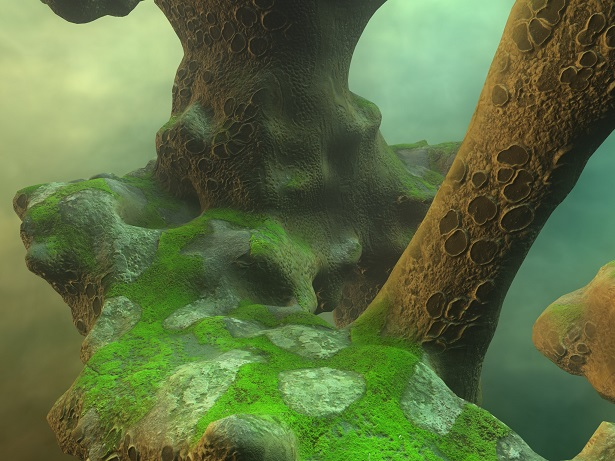
\includegraphics[width=0.5\linewidth]{PICs/cascades_small}
	\caption{Example of a procedural generated rock. \protect\cite{nvidia::cascades}}\label{cascadesFigure}
\end{figure}

\section{Game Mechanics}
Now it comes to the most crucial part of this chapter of PCG because of its leading part in PCGML as a game mechanic — the use of PCG as a game mechanic! This chapter provides an overview of games which are using PCG as a game mechanic and some examples of possible PCG core mechanics.

\subsection{Current Games} \label{pcgMechanicGames}
Many games are using procedurally generated content nowadays, but not all of them are using PCG as a game mechanic. The following sections describe three games which are using PCG as a game mechanic.

\subsubsection{Galactic Arms Race}
Initially, a research project which is a perfect example of PCG-based core mechanics in a game \cite{game::galacticArmsRace}. Galactic Arms Race is a multiplayer space shooter game in which the player needs to complete tasks and missions to progress through the game \cite{game::galacticArmsRace}. To complete tasks and missions, players need to fly around in space and try to kill enemies with different weapons. A highlight of the game is the particle weapon system which is used to defeat enemies whereas weapons are entirely generated by a PCG algorithm using evolutionary AI algorithms to evolve and generate new weapons \cite{pcg::galacticArmsRace}. The AI in Galactic Arms Race creates and evolves weapons based upon actions, strategies, and most used weapons of a player \cite{pcg::galacticArmsRace} \cite{pcg::galacticArmsRace::evolvingContent}. Besides, a player can possess three weapons at a time whereby new evolved weapons are continuously spawned in space and dropped by enemies \cite{pcg::galacticArmsRace::evolvingContent}. Consequently, players need to decide which weapons they want to use and thus feed the AI with information about their preferences \cite{pcg::galacticArmsRace::evolvingContent}. In this case, a player functions as the fitness function of the evolutionary algorithm used by the overall PCG system \cite{pcg::galacticArmsRace::evolvingContent}.

In short, a combination of PCG algorithms and evolutionary AI algorithms produces the novel weapon system which represents the core mechanic of Galactic Arms Race.

\subsubsection{Inside a Star-Filled Sky}
Inside a Star-Filled Sky is an almost entirely procedural generated game \cite{game::insideAStarFilledSky}. The objective for a player is to progress through levels and try to reach one of the highest stages of progress to rule the leaderboard \cite{game::insideAStarFilledSky}. Players need to fight enemies, collect items, power-ups or weapons to defeat enemies and get over to the next level. Each level is generated and can represent the inside of an enemy, item or another entity in the game which gives the player an infinite choice of possibilities on how to play the game. Moreover, players can move in or out of the recursively nested levels, and every collected item or killed enemy change the random seed for generating the next level \cite{pcg::endlessWeb}. Players can even move into their character to increase their power and more than 165000 simple weapon combinations are explorable due to PCG \cite{game::insideAStarFilledSky}.

Summarized, the core mechanic of Inside a Star-Filled Sky is heavily PCG-based and about exploring and progressing through generated levels with the help of generated weapons and items.

\subsubsection{Endless Web}
Is an entirely PCG-based game and thus uses PCG as its core mechanic \cite{pcg::endlessWeb}. It is about fighting the nightmares in human dreams and rescue the trapped ones and thus releasing dreamers from their fears. The central objective of the game is to rescue six dreamers by exploring and make decisions on exploring new areas in the world which affects the parameters of the rescue progress and also the generation of new world parts \cite{pcg::endlessWeb}. For example, if a player kills an enemy then depending on the configuration, it strengthens or weakens an associated challenge and furthermore changes the world \cite{pcg::endlessWeb}.

So, Endless Web's core mechanic is about manipulating the generative space where players influence the changes of the world generation with their chosen decisions on how they are playing the game \cite{pcg::endlessWeb}.

\subsubsection{Other Games}
Games like Black \& White, Diablo, Dwarf Fortress, Elite, Eve Online, Roque, Spelunky or Minecraft are other good examples which made use of PCG and related mechanics as an essential part in their game.

\subsection{Possible Core Mechanics}
There are a few possibilities and use cases for PCG as mechanics in games. As seen, some core mechanics aim at weapon creation and progressing through generated space with the help of generated or altered "helper" mechanisms. Apart from that promising ideas are also other noteworthy ideas:
\begin{itemize}
	\item One exciting idea is about using PCG for multiplayer games as a multi-instance PCG system given by \citep{pcg::futureOfPcgInGames}. A game could use a central PCG system consisting of different and unique systems for each player, and every content generation would affect the PCG systems of other players \cite{pcg::futureOfPcgInGames}.  In that case, the core mechanic of the game would include influencing other players with each others PCG system to work towards a specific goal. For example, a use case would be a collaborative multiplayer game where each content generation causes a new content generated in the other’s player space, and they must find a way to communicate how to achieve a mutual objective \cite{pcg::futureOfPcgInGames}. 
	\item There is a lot of research done in the generation of quests as well. The research of \citep{pcg::questGenerator} introduced generated quests based on analysis of four existing \acp{MMORPG} and their quests. One could create a simulation game where players need to create random quests by doing interaction with the PCG system in order to provide an AI agent with missions which needs to be fulfilled to solve some other problems in the game and thus progress throughout the game.
	\item Another idea is to adapt existing and successful introduced game mechanics with a PCG-backend. For example, one could create a game like Tetris where the core mechanics of rotating a block generates new blocks. For example, every time the player rotates the block, the next block will be altered with evolutionary algorithms and changes their shapes to increase the difficulty. Moreover, the system could adapt its difficulty to the player's skills regarding the success or failure rate of using the new blocks to maintain an acceptable experience.
\end{itemize} 

%
% ------------------------------- NEW CHAPTER ------------------------------- %
%
\clearpage
\chapter{\acl{ML}} \label{chapter::machineLearning}
\ac{ML} is such a vast topic so that a detailed explanation of every type, approach, method, and model used in ML would go beyond the scope of this thesis. Therefore, the next sections will describe essential subjects of ML which can be useful to understand its further use in PCGML. 

However, let us ask a question first: What is the difference between ML and AI and what is ML about actually? The fact is, there is no difference between ML and AI. In particular, ML developed from fields of research in AI and is thus a subset of AI. It concentrates on using mechanisms to learn from given data where data represents experience for a given problem. For instance, a famous example of machine learning is an application where the machine can distinguish between apples and pears with the help of a given dataset of features for both apples and pears \cite{ai::book}. 

\section{Types of Learning Problems}
Machine learning consists out of three main types which all address a different kind of problem to solve and goal to achieve. One can classify types of supervised learning, unsupervised learning and reinforcement learning \cite{ml::book::developer}. Each of them functions as a solver to a specific task or problem where it fits best and creates the desired results.

\subsection{Supervised Learning}
This type of learning is a task-driven approach of ML \cite{ml::book::developer}. Its primary application is predicting or approximating data based on existing historical or empirical values where the answer to the problem is already known \cite{ai::book}. The previously described problem of classifying apples and pears is a supervised learning problem which is solved by predicting the specific fruit or also referred to as a class \cite{ml::book::developer}. In this case, we would provide a sample set of real data with features for both fruits and classify each feature to a specific fruit. With this, the algorithm links the given features to a specific result and can predict those fruits based on a given test set \cite{ml::book::developer}. A training and test set could exist out of a bunch of pictures or other specific features described with numeric values in a table for each fruit. Hence, the reason why this is called supervised learning is that an ML algorithm is provided with data labels and therefore knows what to learn \cite{ai::book}.

Typical applications for supervised learning are, for example, image recognition and classification, spam detection, pattern detection, speech recognition, \ac{NLP}, sentiment analysis or forecasting \cite{ml::book::algorithms}.

\subsubsection{Regression}
A statistical process is the basis of this supervised learning technique where particular probability distributions of a given training data control the prediction output \cite{ml::book::developer}. In specific, a regression algorithm is processing independent and dependent variables of a given problem and build relationships between them which are furthermore used to predict the correct answers of a given unknown set \cite{ml::book::developer}. Independent variables are describing features and dependent variables the meaning or outcome of a regression problem. Usually, regression algorithms are applicable when the output values are constant prediction problems like for example, the predicted time of completion for a game level based on, e.g., the current player position \cite{ai::book}.

Some use cases where concepts of regression algorithms can be applied are, e.g., for imitation and prediction of a player's behavior or player preference learning \cite{ai::book}. Some popularly used algorithm for regression are the linear or polynomial regression, \ac{ANN} or \ac{SVM}. \cite{ai::book}

\subsubsection{Classification}
Addresses problems where classification transition of independent values into specific values is needed \cite{ai::book}. The famous problem of classifying and distinguish apples and pears from each other falls into this section.

Like regression algorithms, classification algorithms are applicable for imitation and prediction of a player's behavior, such as prediction of completion time \cite{ai::book}. However, in this case, the possible outputs are specific values or classes like slow, average or fast instead of continuous values \cite{ai::book}. Some popularly used algorithm for classification are, e.g., \ac{ANN}, decision tree, random forests, \ac{SVM}, \ac{KNN} or ensemble learning \cite{ai::book}.

\subsection{Unsupervised Learning} \label{ML::unsupervisedLearning}
In contrast to supervised learning, the base of unsupervised learning is a data-driven approach where the algorithm has no information about the meaning or value of any sample and needs to infer it automatically \cite{ml::book::developer}. Hence, an unsupervised learning algorithm gets so-called unlabeled data without having a specific relationship to the target output and finds unknown structures and pattern in that set \cite{ai::book}. Thinking about the apples and pears example, then an algorithm would try to detect that there are two different types or classes in the dataset instead of predicting if it is an apple or a pear.

Typical applications for unsupervised learning are object segmentation, similarity or pattern detection, automatic labeling, pre-training of supervised algorithms or preprocessing data such as data compression, noise smoothing or outlier detection \cite{ml::book::algorithms} \cite{ai::book}.

\subsubsection{Clustering}
For example, solves the previous described apples and pears problem by clustering apples and pears out of the given training set with features of both fruits. Based on the trained knowledge due to the training set, it can differentiate new and unknown samples into either apples, pears or an entirely new class \cite{ai::book}. In detail, clustering algorithms are looking for similarities between given features and values, and by doing this, they are inferring a relationship between them and thus separate specific classes \cite{ml::book::developer}.

Popularly used algorithms for clustering are, e.g., K-Means, \acp{NN} or \acp{HMM}  \cite{ml::book::developer}.

\subsection{\acl{RL}}
In short, \ac{RL} is a goal-oriented approach where an AI tries to reach a goal with the best strategy \cite{ml::book::developer}. RL uses so-called agents who are used to get feedback or specific states of an environment which is further used to learn and improve new decisions based on taken decisions \cite{ml::book::developer}. Inspired by the way humans and animals learn to take decisions, it aims at rewarding the algorithm for good behavior and thus leads it towards the best knowledge and output \cite{ai::book}. 

In general, RL makes use of a bit of supervision in the form of feedback for an action executed by an agent \cite{ml::book::statistics}. Among experts, this feedback exists as the reward for actions in RL algorithms \cite{ml::book::statistics}.  The tricky part is that RL usually consists of following decisions and every chosen action — chosen out of a set of actions — by an agent is changing the environment which usually makes it difficult to train a model \cite{ml::book::statistics}. Hence, an agent executes different decisions in a loop and is looking for the highest total reward for its sequence of actions since it will always want to increase its total reward. \cite{ai::book} With this strategy, an RL algorithm is getting better and better over time in solving a specific problem until it found the best solution.

During the last years, RL algorithms have been used to learn an AI how to play classical games, find the best strategy to win a game, learn an AI how to walk and many other applications \cite{ml::book::algorithms}. Algorithms include \acp{NN}, deep neural networks, Q-Learning or Markov decision process. \cite{ml::book::statistics}

\subsection{Generative versus Discriminative Models}
Another viewpoint to differ ML models is to group them into generative and discriminative models. Both of them have different applications and advantages. As the name of generative models suggests, their application is for data generation problems instead of simple label predictions problems \cite{ml::book::nnProgrammingTF}. This fact infers that there is a difference in their underlying learning approach which is the crucial point of the distinction \cite{ml::book::nnProgrammingTF}. Discriminative models include \acp{NN}, decision trees, random forests or \acp{SVM} whereas generative models include \acp{GAN}, Autoencoders such as \acp{VAE}, \acp{LSTM} or \acp{RNN} \cite{ml::book::nnProgrammingTF}. 

In particular, the primary distinguishing feature between the models is their approach on how to learn the relationships of the training attributes to either the labels or all the other attributes as a whole. With this said, discriminative models try to learn the conditional relationship between the features and the labels, denoted as $P(Y|X)$, whereas generative models try to learn the joint probability distribution of the whole data and then infer the conditional relationship, denoted as $P(X,Y)$ \cite{ml::book::nnProgrammingTF}.

\section{Development} \label{mlDevelopment}
Developing an easy to use AI needs to be a well-structured and planned process. Especially, when using ML as a focus of interaction, it is even more important to be well-prepared. For this reason, this chapter addresses some design considerations about developing user-friendly AI systems in games, as well as standard pitfalls to keep in mind, standard procedures for data preprocessing and possibilities of how to use ML algorithms in two commonly used game engines.

\subsection{Design Considerations}
Someone cannot just develop a new novel AI system and expect to create a whole new experience — it needs to have a thoughtful plan how to achieve new experience \cite{ai::gameDesign}. Firstly, it is useful to think about the MDA framework, which was described in Chapter \ref{gameMechanicsChapter}, because an AI-based game is often tightly integrated into its game mechanics and therefore it is necessary to make no mistakes in the first place to fulfill playability and emerging experience \cite{ai::gameDesign}. 

Here are some critical considerations for AI-based games described by \citep{ai::gameDesign} which are also worth noting for implementing an ML-based AI system: 
\begin{itemize}
	\item First, develop a rough design of the game system and then model the AI system upon that game system or vice versa \cite{ai::gameDesign}. In particular, for AI-based games, the AI system should support the designed core experience of the game \cite{ai::gameDesign}.
	\item An AI should provide possible exploration and allow a player to experiment with it which means it should be robust enough and not lead to game crashes or misbehavior \cite{ai::gameDesign}. 
	\item Avoid a too mechanical and unnatural player experience with an unpredictable system \cite{ai::gameDesign}.
	\item The environment of an AI-based game should be observable for an AI system which means it should be able to access states of different game entities at any time \cite{ai::gameDesign}. Consequently, game states should be described in a way so that an AI system can easily access and read it \cite{ai::book}.
	\item A system should be as accessible and transparent as possible for a player so that a player will not be overwhelmed by the system and its possibilities \cite{ai::gameDesign}. Notably, an interactive ML system as an AI system in the game could be a confusing thing for a player if it, e.g., exposes too much information \cite{ai::gameDesign}. That is of particular importance when using \ac{RL} as the backbone AI agent algorithm.
	\item Provide ways for emergent gameplay with the help of the AI system with, e.g., possible strategies which can be applied to the system \cite{ai::gameDesign}. 
\end{itemize}

Lastly, the discussed issues and considerations in Chapter \ref{mechanicsConsiderationsPCGandML} also apply for the implementation of an ML-based AI agent.

\subsection{Common Pitfalls}
Following pitfalls are commonly occurring problems when implementing and training machine learning models for a specific problem.

\subsubsection{Under- and Overfitting}
ML models are used to approximate unknown output based on given training data \cite{ml::book::algorithms}. When talking about fitting, then it is referred to fit a model to a given training set and its features which are used to train the model. This set can consist of many independent variables and different entries which can create some issues:
\begin{itemize}
	\item \textbf{Underfitting}: Happens when the training set for the model consists of too less information or independent variables \cite{ml::book::algorithms}. In that case, the model is not able to capture the dynamics of the values \cite{ml::book::algorithms}.
	\item \textbf{Overfitting}: Is exactly the opposite of underfitting. When a model is over-fitted then it is fed with too much information and variables so that it is not able to generalize the dynamic relationship of variables during the training \cite{ml::book::algorithms}.
\end{itemize}

Therefore, a right amount of information for the training of a machine learning model should be provided to achieve an excellent fitted model. A method to check and prevent the model from being over or under-fitted is the technique of validation such as cross-validation which helps to detect those problems \cite{ml::book::algorithms}.

\subsubsection{Curse of Dimensionality}
This problem often occurs when the training set is smaller than the number of feature variables, or also called the dimensions of a set, which are used to train a model \cite{ml::book::algorithms}. In this case, if the number of features increases then the performance of the model gets dramatically reduced \cite{ml::book::algorithms}. Possible ways to prevent and solve this problem are, e.g., a decrease of dimensions or providing more training data \cite{ml::book::algorithms}.

\subsection{Data Preprocessing} \label{ML::dataPreprocessing}
A standard procedure in ML is the technique of data preprocessing so that data values are consistent with each other. Table \ref{table::PCGML::devExample::data} shows a simple example data table which could be usable for the systems training. The table’s data can contain any discrete or continuous values which could originate from any decoded non-numerical data.
\begin{table}[!htbp]
	\centering
	\begin{tabular}{|c|c|c|c|c|}
		\hline
		\textbf{V\textsubscript{1}} & \textbf{V\textsubscript{2}} & \textbf{...} & \textbf{V\textsubscript{n}} \\ \hline\hline
		 2.1         & A           & ...          & 100         \\ \hline
		 5           & B           & ...          & 64          \\ \hline
		 ...         & ...         & ...          & ...         \\ \hline
		-0.958         & A         & ...          & 986         \\ \hline
	\end{tabular}
	\caption{Machine learning training data example.}
	\label{table::PCGML::devExample::data}
\end{table}

\subsubsection{Encoding}
For example, if the data set provides categorical data like the values for \textbf{V\textsubscript{2}}, as shown in Table \ref{table::PCGML::devExample::data}, then this data needs to be encoded, so it does not differ from the other data values. This procedure is a standard procedure in the data preprocessing for training an ML model and can be done with so-called "One Hot Encoding." Table \ref{table::PCGML::devExample::oneHotEncoder} shows an example of what an one hot encoder does with categorical data as provided by \textbf{V\textsubscript{2}}. 
\begin{table}[!ht]
	\centering
	\begin{tabular}{|c|c|c|c|c|}
		\cline{1-1} \cline{3-5}
		\textbf{V\textsubscript{2}} &  & \textbf{V\textsubscript{2}\textsuperscript{1}} & \textbf{V\textsubscript{2}\textsuperscript{2}} & \textbf{V\textsubscript{2}\textsuperscript{3}} \\ \hhline{=~===}
		A           & $\longrightarrow$         & 1           & 0           & 0           \\ \cline{1-1} \cline{3-5} 
		B           & $\longrightarrow$         & 0           & 1           & 0           \\ \cline{1-1} \cline{3-5} 
		C           & $\longrightarrow$         & 0           & 0           & 1           \\ \cline{1-1} \cline{3-5} 
	\end{tabular}
	\caption{One hot encoder example.}
	\label{table::PCGML::devExample::oneHotEncoder}
\end{table}
The new values generated by the one hot encoder replace the old categorizes values, and the data set is ready to go. It is essential to keep in mind that this encoding can cause the curse of dimension if there are too many categories in the data.
\begin{table}[!ht]
	\centering
	\begin{tabular}{|c|c|c|c|c|c|c|}
		\hline
		\textbf{V\textsubscript{1}} & \textbf{V\textsubscript{2}\textsuperscript{1}}& \textbf{V\textsubscript{2}\textsuperscript{2}}& \textbf{V\textsubscript{2}\textsuperscript{3}} & \textbf{...} & \textbf{V\textsubscript{n}} \\ \hline\hline
		2.1         & 1   & 0   & 0       & ...          & 100         \\ \hline
		5           & 0   & 1   & 0       & ...          & 64          \\ \hline
		...         & ... & ... & ...     & ...          & ...         \\ \hline
		-0.958      & 0   & 0   & 1       & ...          & 986         \\ \hline
	\end{tabular}
	\caption{Encoded training data example.}
	\label{table::PCGML::devExample::data_encoded}
\end{table}

\subsubsection{Feature Scaling}\label{chapter::ml::feature_scaling} %see http://sebastianraschka.com/Articles/2014_about_feature_scaling.html#about-standardization
Feature scaling is a crucial process in data preprocessing. It helps to make unbalanced datasets more manageable for the training and especially during backpropagation or error correction \cite{ml::book::developer}. The occurring problem is that most optimizer functions in ML, for example in \ac{KNN}, are using Euclidean distance to measure the cost of, e.g., a prediction which is then used to calculate the delta for backpropagation. Now, the main problem with taking the Euclidean distance is that it is getting easily biased with, e.g., significant values in the dataset which furthermore dominate all the other ones. For example, the last attribute in column \textbf{V\textsubscript{n}} in Table \ref{table::PCGML::devExample::data_encoded} is an immense value which would create a more significant delta for all other attributes during backpropagation. Now, there are two commonly used methods to avoid this problem:
\begin{itemize}
	\item \textbf{Standardization}: Aims to balance the dataset so that its distribution is closer to a normal distribution \cite{ml::book::developer}. The formula for standardization is: $z={\dfrac{x - \mu}{\sigma}}$.
	\item \textbf{Normalization}: Aims to transform the distribution of the dataset into a range between 0 and 1 \cite{ml::book::developer}. The formula for normalization is: $x_{norm}={\dfrac{x - x_{min}}{x_{max}-x_{min}}}$.
\end{itemize}
Applying normalization to the example dataset of Table \ref{table::PCGML::devExample::data_encoded} results in a dataset shown in Table \ref{table::PCGML::devExample::data_normalized}.
\begin{table}[!ht]
	\centering
	\begin{tabular}{|c|c|c|c|c|c|c|}
		\hline
		\textbf{V\textsubscript{1}} & \textbf{V\textsubscript{2}\textsuperscript{1}}& \textbf{V\textsubscript{2}\textsuperscript{2}}& \textbf{V\textsubscript{2}\textsuperscript{3}} & \textbf{...} & \textbf{V\textsubscript{n}} \\ \hline\hline
		0.513      & 1   & 0   & 0       & ...          & 0.039         \\ \hline
		1           & 0   & 1   & 0       & ...          & 0          \\ \hline
		...         & ... & ... & ...     & ...          & ...         \\ \hline
		0      & 0   & 0   & 1       & ...          & 1         \\ \hline
	\end{tabular}
	\caption{Normalized training data example.}
	\label{table::PCGML::devExample::data_normalized}
\end{table}

\subsection{Game Engine Plugins} \label{chapter::mlPluginsGameEngines}
Indeed, all the different machine learning models or the one which applies to the game prototype of this thesis could be self-implemented. However, there are other people out there who have already implemented and improved their implementations which are a good starting point when implementing a PCGML game mechanic. As discussed at the beginning of the thesis, it is going to focus on an implementation in commonly used game engines which is the reason why to envisage the two most used free to use game engines nowadays.

\subsubsection{Unity}
Unity made an incredible effort in its research and use of machine learning in their engine in the last year \cite{unity::ml}. They recently released a beta version of an open-source ML agents plugin that enables games to train an AI with \ac{RL}, imitation learning, neuroevolution or other ML methods \cite{unity::mlGithub}. The base of the plugin is Google’s open-source ML framework \acf{TF} \cite{api::tensorFlow} which is accessible via a simple-to-use Python \ac{API} \cite{unity::mlGithub}. They are also providing essential instructions and documentary for the usage of their plugin which is a promising, definite and significant advantage when implementing the PCGML game mechanic.

\subsubsection{Unreal Engine 4}
At the time of writing this section, there is no available officially announced ongoing plugin or feature development for ML in \ac{UE4}. However, there are others who were concerned about the missing feature of ML in UE4. For this reason, \citep{ue4::tensorFlowPlugin} created an open-source \ac{TF} plugin for UE4 which implements a Python API accessible interface based on a fork of a UE python plugin. Indeed, there are also some other plugins available via UE4's marketplace such as a Q-Learning plugin, but there do not look that promising as \citename{ue4::tensorFlowPlugin}'s \ac{TF} plugin. Also, provided documentation and guidance on how to use the plugin leads it to a tolerable option besides to Unity’s ML agent plugin.

\section{Game Mechanics}
It is unclear which games used specific methods of ML for a game mechanic because there are not any research paper or published articles about, i.e., game companies who talked about using ML for their mechanics. Nevertheless, there is a research focus on AI-based games, including game mechanics which can be adapted with ML and is therefore used to come up with ideas for ML game mechanics. 

\subsection{Current Games}
Two games which use AI as a core mechanic were already described in Chapter \ref{pcgMechanicGames} and are the games Endless Web and Galactic Arms Race. Both making use of a PCG and AI mixture mechanic where the AI generates new world segments based on game world states \cite{pcg::endlessWeb} or new weapons based on player preferences \cite{pcg::galacticArmsRace}. These games are going to be first reference points and inspiration when implementing a PCGML game mechanic. Other games which used ML techniques as a mechanic were, e.g., Black and White and Creatures \cite{ml::mostInfluentalAiGames}. 

\subsubsection{Black and White}
The player is in control and owns a creature who can be trained to do things for the player. They used techniques such as decision trees and neural networks to train and learn it the prediction of a player's action \cite{ml::gamasutra::ml} \cite{ml::mostInfluentalAiGames}. In particular, the belief-desire-intention approach was used to implement the creature's behavior \cite{ml::mostInfluentalAiGames}. The creature's training happens due to a player’s reaction upon the creature's executed actions which therefore follows the rules of RL where the creature would like to achieve the best total reward for its behavior \cite{ml::gamasutra::ml}.

\subsubsection{Creatures}
That is a game where players need to hatch animals and try to teach them how to behave and survive in their world \cite{ml::mostInfluentalAiGames}. As well as Black and White, Creatures also used neural networks to teach and learn animals how to behave based on a player's input \cite{ml::mostInfluentalAiGames}.

\subsection{Possible Mechanics}
\citep{ai::aiBasedGameDesignPattern} introduced nine design patterns, summarized in Table \ref{AI-basedMechanicsDesignPattern} which illustrates ways to develop game mechanics based on AI techniques and furthermore to create AI-based games. Following sections describe some examples of possible mechanics or core mechanics with ML, based on \citename{ai::aiBasedGameDesignPattern}'s design patterns.
\begin{table}[!ht]
	\centering
	\resizebox{\textwidth}{!}
	{%
		\begin{tabular}{|p{2.1cm}||p{8cm}|p{4cm}|p{4cm}|}
			\hline
			\multicolumn{1}{|c||}{\textbf{Pattern Name}} & \multicolumn{1}{c|}{\textbf{Description}} & \multicolumn{1}{c|}{\textbf{Role of Player}} & \multicolumn{1}{c|}{\textbf{Role of AI}} \\ \hline\hline
			\textbf{Visualized} & Visualization of AI system states so that gameplay revolves around state manipulation & Observation and manipulation of an AI system & Shows states and gives information \\ \hline
			\textbf{Role-Model} & Player needs to imitate AI agents & AI system imitation & Shows actions and behavior, e.g., as a puzzle \\ \hline
			\textbf{Trainee} & AI system needs to be trained to perform gameplay tasks & Teacher for AI system & Learns desired behavior \\ \hline
			\textbf{Editable} & Player needs to change elements of an AI agent which are related to gameplay & Observation and manipulation of the AI & Handles changes and shows a new behavior \\ \hline
			\textbf{Guided} & Player partly assists or guides an AI agent who is threatened  by a problem & Guidance and management of the AI & Acts on its own but mostly does what the player wants \\ \hline
			\textbf{Co-Creator} & Player and AI work together as equal partners & Learns how to play the game with AI assistance & Acts as co-creator and assistance for the player \\ \hline
			\textbf{Adversary} & Player needs to defeat an AI system & Adapts to an AI and defeats it & Tries to defeat the player \\ \hline
			\textbf{Villain} & Player needs to defeat an AI system whereas AI system does not want to defeat the player & Adapts to an AI and try to defeat it & Acts as villain and mob the player \\ \hline
			\textbf{Spectacle} & AI which implements a complex system and the player needs to observe, interact or overcome it & Observation, interaction or manipulation of the system & Spectacles and simulates the system \\ \hline
		\end{tabular}%
	}
	\caption{AI-based game mechanics design pattern \protect\cite{ai::aiBasedGameDesignPattern}}
	\label{AI-basedMechanicsDesignPattern}
\end{table}

\subsubsection{AI as Role-Model}
For example, a game in which a player needs to follow an AI to solve quests or missions. Based on the players progress in each quest and imitation level, the AI adjusts its solution of solving the current or a new problem and provides the player with either a less competitive or harder solution and reward. Hence, player experience is adapting due to player behavior learning and predicting an appropriate difficulty level. For instance, a quest could be following or remembering the path of the AI to a treasure whereas built-in traps are crossing the way. Hypothetically, if the player cannot remember and succeed the path after, e.g., three times, then the AI shows a new and less challenging path to a less rewarding treasure.

\subsubsection{AI as Trainee}
Is one of the most promising design pattern since it revolves around teaching an AI different things whereby it fits perfectly for using ML methods. As introduced before, the games Black and White and Creatures are using precisely this kind of pattern for implementing their creature behavior. A game could use a mechanic the same way and introduce new mechanics on how to interact and use the AI agent by teaching it how to behave in specific situations. A simple idea would be a teaching game in which the player needs to educate fighters to defeat enemies. Alternatively, a tower defense game in which the player uses defense entities to teach an ML agent first target preferences.
	
\subsubsection{AI as Co-Creator}
An exciting base idea of a co-creator AI game would be a split-screen game in which the player plays on one side and the AI agent on the other side. The gameplay would be symmetrical, and everything a player does, the AI will try to imitate. In doing so, the player needs to do things to complete challenges whereas done actions affect the AI agents space and vice versa. For example, a challenge could be pushing a button which only exists in the space of the AI but opens, e.g., a door in the player's space. Therefore, the player would need to behave in a specific manner to lead the AI towards the button to progress through the game.

%
% ------------------------------- NEW CHAPTER ------------------------------- %
%
\clearpage
\chapter{\acl{PCGML}}
A purpose for research in AI-based PCG methods like PCGML was to invent algorithms which can create and generate content of the same type and style based on existing content with or without human involvement \cite{ai::book} \cite{pcgml::paper}. In general, \citep{pcgml::paper} defined PCGML as ''the generation of game content using machine learning models trained on existing content.'' 

On this account, different research was and is carried out to generate music, sound effects, images, textures, worlds or levels \cite{ai::book}. Research showed that ML-backed PCG methods are working well for music and images but are facing some issues when it comes to world or level generation because of its necessity of playability to create an adequate experience for the player \cite{ai::book}. Thus, the generation of gameplay content raised challenges, demanding further research for solving such problems \cite{ai::book}. Therefore, PCGML approaches were not used in games yet. Another reason is that there is often not enough game content available to train a PCGML model for a specific content generation problem \cite{ai::book}. 

The next chapters introduce the difference to usual PCG, use cases of PCGML, some developmental features used in other research and explains how PCG and ML work together to generate new content in an example. Overall, this chapter is not going into many details since all essential cornerstones of PCGML where discussed and introduced in the previous chapters.

\section{Difference to \acl{PCG}}
Usual PCG and PCGML have in common their hand-made algorithms, parameters, and constraints made by developers \cite{pcgml::paper}. Typically, designers would use existing game data and content as foundation for new ideas and develop generators for creating new material on top of that inspiration, whereas PCGML itself can get utilize existing data to develop new content and thus assist the designer \cite{pcgml::paper}. So, the basic idea is to train the PCGML model on various but similar game content and produce new one \cite{pcgml::paper}. 

In contrast, different PCG algorithms might use ML for evaluation, but their content generation process entirely relies on their specific domain space rather than a trained model space \cite{pcgml::paper}. For example, experience-driven PCG relies on models of player experience whereas PCGML models can use existing balanced domain-specific content to create new one \cite{pcgml::paper}.

\section{Use Cases}
The focus of PCGML is to generate new content based on training with existing content. For this reason, PCGML can be used mainly for adaption, reparation, evaluation, critique or analysis of new content but also for general PCG tasks like autonomous generation, co-creative, and mixed design or data compression \cite{pcgml::paper}.
\begin{itemize}
	\item \textbf{Autonomous Generation}: Is one of the primary applications for PCGML because it can generate game content without human input which is especially useful when online content generation is needed \cite{pcgml::paper}. Also, a designer could create, e.g., a set of levels and for a model's training to create new and novel but similar levels with the help of the PCGML system \cite{pcgml::paper}.
	\item \textbf{Co-creative and Mixed-initiative Design}: This use case focuses on the collaboration between designers and the PCGML algorithm \cite{pcgml::paper}. For instance, the algorithm could generate new content based on provided examples as a draft for the designer who could polish and finish the drafted content afterward.
	\item \textbf{Data Compression}: PCGML offers significant potential for data compression with the help of ML. Extracting specific dimensions of game content can save data size and would allow more efficient storage \cite{pcgml::paper}.
	\item \textbf{Recognition}: This is where PCGML stand out from the conventional PCG algorithms. Its  recognition capabilities make it possible to analyze, evaluate, adapt, critique or repair either existing, new designed, player created or algorithm generated game content \cite{pcgml::paper}. 
	\item \textbf{Repair}: In particular, reparation of a designed or generated content can be a useful tool. For example, during generation or learning time, the algorithm could check for, e.g., playability of a level and repair it immediately or suggest a fix \cite{pcgml::paper}.
\end{itemize}

\section{Development Considerations} \label{PCGML::devConsiderations}
There are some unique development considerations to take when someone wants to make use of PCG via ML for game elements. In general, every design consideration, possible issue, pitfall and best practices described and discussed in Chapters \ref{pcgDevelopment} and \ref{mlDevelopment} will apply for implementing PCGML algorithms. Furthermore, an initial examination of the data representation for the training set during the ML model’s training could be helpful. On this account, the research of \citep{pcgml::paper} showed that specific datasets with significant difference share possible training methods to obtain excellent and practical generation results. \citep{pcgml::paper} further organized their used datasets into sequence-, grid- and graph-based data. They made that distinction because it fitted best with their main problem addressed in the paper which was primarily about generating levels.

\subsection{Machine Learning Models}
Because PCGML generates new content based on existing one, it seems reasonable that the models which fit best for most of the PCGML tasks are generative ML models.

This is confirmed by the fact that the primarily used training models in \citename{pcgml::paper}'s research of using PCGML for, e.g., level generation, were based on the paradigm of \ac{NN} and are models such as \acp{CNN}, \acp{LSTM}, Markov models like N-grams or multi-dimensional Markov chains, Bayes models, Autoencoders, Clustering or Matrix factorization. Nevertheless, not all of them are pure generative models which means that discriminative models can be a better fit sometimes.

\section{Development Example} \label{PCGML::devExample}
There is no right or wrong proceeding in the generation process for PCGML. PCGML is a very new paradigm in the content generation community, and its research results drive the right or wrong approaches. With this in mind, the PCGML generation process can take shape in any form, and someone should do what fits best for a given problem.

This section explains a development example of a generation process for data with depending attributes realized with discriminative models as ML backend. However, Chapter \ref{chapter::gamePrototype} provides the detailed development walk-through of a PCGML system. For this example, a data’s structure example for a PCGML system provides the Figure \ref{fig::PCGML::devExample::sequenceBase}. As it is a sequence of data, there is a connection between all variables. In the figure, the node "S" represents a start value, and all other nodes represent independent attributes or features. 
\begin{figure}[!htbp]
	\centering
	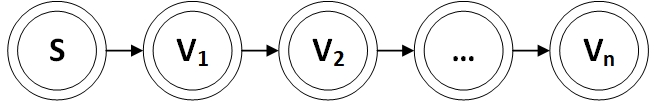
\includegraphics[width=0.5\linewidth]{PICs/PCGML_development_example_sequence_base}
	\caption{Basic training data for a PCGML system. }\label{fig::PCGML::devExample::sequenceBase}
\end{figure}
Figure \ref{fig::PCGML::devExample::sequenceWithModels} shows dashed rectangles around the attributes which indicates separately trained ML models for each attribute pairs. 
\begin{figure}[!htbp]
	\centering
	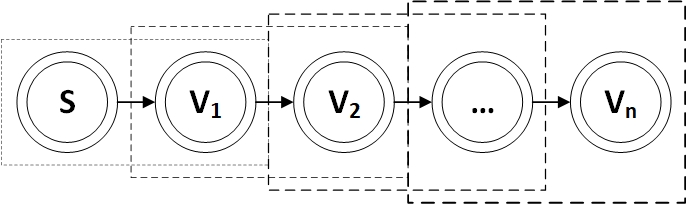
\includegraphics[width=0.55\linewidth]{PICs/PCGML_development_example_sequence_with_models}
	\caption{Basic training data for a PCGML system with shown ML models.}\label{fig::PCGML::devExample::sequenceWithModels}
\end{figure}
It is worth noting that values do not need just one predecessor, but can have multiple which would change the dashed rectangles, ML models and their associated variables shown in Figure \ref{fig::PCGML::devExample::sequenceWithModels}.

\subsection{Data}
First of all, it is necessary to come up with efficient and sufficient data for the system’s training. Depending on the variables, more or less data is needed for the model. For example, a data structure with around ten features would probably need at least 100 data rows to train the ML model properly. In particular, there is an unofficial rule of thumb that the dataset should be ten time times bigger than the provided number of parameters. As soon as the data is available, preprocessing for the training should be applied, following the steps described in Chapter \ref{ML::dataPreprocessing}.


\subsection{Training}
After provision and preprocessing of the dataset follows the training. Training can happen with different training models as described in Chapter \ref{PCGML::devConsiderations}. For example, the use of an ANN could be a suitable training model for a given example dataset. In the scenario of previous described training data, the \acp{NN} would be trained for each pair of values to output the next value in the sequence. Figure \ref{fig::PCGML::devExample::NNbasic} shows an example of a simple feed-forward \ac{NN} where the start value and the first variable are used to predict the second variable. The neurons in all \acp{NN} shown in this thesis will follow the color scheme introduced in Figure \ref{fig::neuron_legend}. 
\begin{figure}[!htbp]
	\centering
	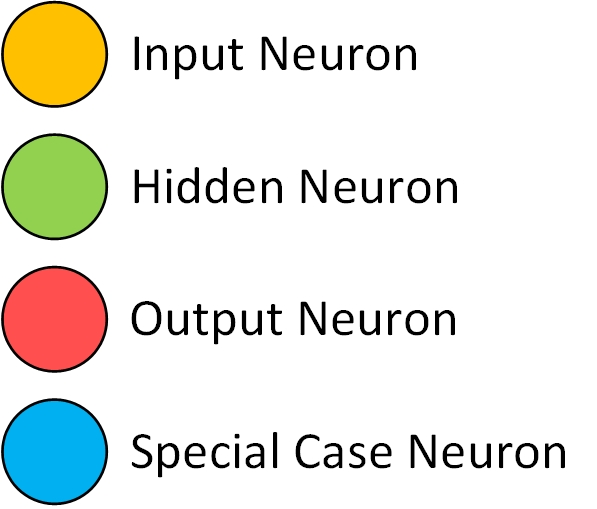
\includegraphics[width=0.3\linewidth]{PICs/NNs/neurons_legend.jpg}
	\caption{Neuron legend for all neural networks in this thesis.}\label{fig::neuron_legend}
\end{figure}
\begin{figure}[!htbp]
	\centering
	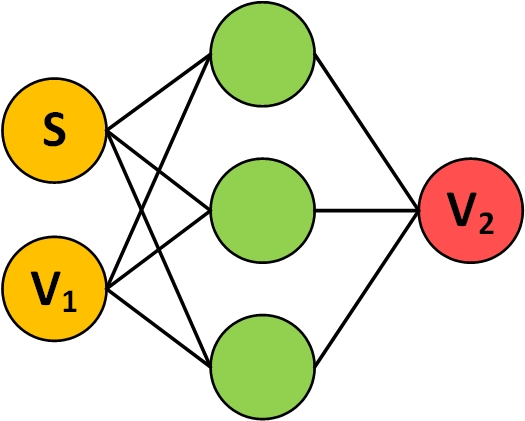
\includegraphics[width=0.3\linewidth]{PICs/NNs/PCGML_development_example_NN_basic}
	\caption{Basic feed-forward neural network to output a variable based on given input variables.}\label{fig::PCGML::devExample::NNbasic}
\end{figure}

In specific, the training of several \acp{NN} for every following variable of the data sequence is necessary to output and generate a complete result. Another possibility to use \acp{NN} would be to make use of the so-called "Softmax" function which outputs the categorical distribution or probability distribution of a variable. With this probability, it can generate and train the following variables. Figure \ref{fig::PCGML::devExample::NNwithSoftmax} shows this kind of NN with an example probability distribution in the output layer.
\begin{figure}[!htbp]
	\centering
	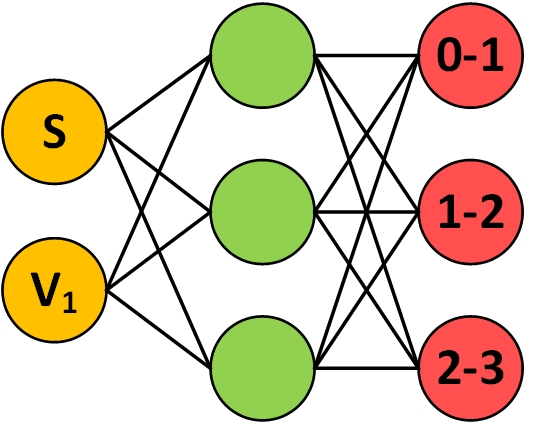
\includegraphics[width=0.3\linewidth]{PICs/NNs/PCGML_development_example_NN_categorical_distributions}
	\caption{Neural network with an probability distribution example in the output layer.}\label{fig::PCGML::devExample::NNwithSoftmax}
\end{figure}


\subsection{Generation}
The next step in developing a PCGML system after the correct training of the model is the generation process. This process can differ depending on the used training model, given data and data representation. For example, the system could generate the first variable and get the other ones from the model. Alternatively, it could generate any variable in the sequence and retrieve the others from that one. Alternatively, it could make use of the probability distribution output by the Softmax function which leads the variables and generates a new piece of game element. As mentioned at the beginning of this chapter, there are no standards in the PCGML generation process, and someone can make use of every possibility which is provided by the system.
 
%
% ------------------------------- NEW CHAPTER ------------------------------- %
%
\clearpage
\chapter{Possible Game Mechanics} \label{chapter::possibleGameMechanics}
The initial ideas on how to use PCGML as a game mechanic were created by \citep{pcgml::paper}. They came up with the following seven different ideas based on the AI-based game design pattern described in Chapter \ref{AI-basedMechanicsDesignPattern}:
\begin{itemize}
	\item \textbf{Role-Model}: "A \ac{PCGML} system replicates content which is generated by players of various levels of skill or generates content suitable for players of certain skill levels. New players are trained by replicating the content or by playing the generated content in the form of generative tutorial." \cite[p. 13]{pcgml::paper}
	\item \textbf{Trainee}: "The player trains a \ac{PCGML} system to generate a piece of necessary content (e.g., part of a puzzle or level geometry)." \cite[p. 13]{pcgml::paper}
	\item \textbf{Editable}: "Rather than training the AI to generate the missing puzzle piece via examples, the player changes the internal model’s values until acceptable content is generated." \cite[p. 13]{pcgml::paper}
	\item \textbf{Guided}: "The player corrects the \ac{PCG} system’s output to fulfill increasingly difficult requirements. The \ac{AI}, in turn, learns from the player’s corrections, following the player’s guidance." \cite[p. 13]{pcgml::paper}
	\item \textbf{Co-Creator}: "The player and a \ac{PCGML} system take turns in creating content, moving towards some external requirements. The \ac{PCGML} system learns from the player’s examples." \cite[p. 13]{pcgml::paper}
	\item \textbf{Adversary}: "The player produces content that the \ac{PCGML} system must replicate by generation to survive or vice versa in a “call and response” battle." \cite[p. 13]{pcgml::paper}
	\item \textbf{Spectacle}: "The \ac{PCGML} system is trained to replicate patterns that are sensorically impressive or cognitively interesting." \cite[p. 13]{pcgml::paper}
\end{itemize}
These ideas were used to come up with more ideas on how to use PCGML as a game mechanic in modern video games.

\section{Concepts and Development Evaluation}
Each of the following chapters describes an idea of a PCGML mechanic followed directly with a development related evaluation. It is to say that in general, the central issue in the implementation of the PCGML system will be the training data for the ML model rather than the PCG output itself. Proper training for the ML model requires the right amount of training data to function as intended. The size of the right dataset can differ from application to application based on the given values as dependencies for an output. 

Moreover, each idea has the advantage of PCGML that it can generate similar elements as used during training time, the possibility of changing the training set and thus the output. Also, there is no need for finetuning to generate a broad range of elements in contrast to standard PCG algorithms. For this reason, as it is the implication of using PCGML, these described advantages are not mentioned in the evaluation. Also, the provision of playability is a necessary criterion which contributes equally to each game mechanic.

\subsection{Rules and Behavior} \label{idea::rulesAndBehavior}
A possible idea is a PCGML system which generates rules for a strategy game. A generic and modular strategy game offers the perfect foundation for generating its internal rules and behavior based on its internal elements. In particular, a strategy game mostly exists out of different sequences of actions emerging from new elements in the game which furthermore lead the game in a specific direction. All of those available actions have a different effect in the game whereas the effects can be changed with other appropriate effects causing different changes during the game. More particular, the design of a strategy game can introduce more game elements than used in the game itself. This kind of game element preselection often arises in cardboard games where players need to choose the available cards in advance which affects the flow of the game. For example, if a game provides the players with 25 different elements and just ten elements are used in the game, then it provides, regarding the mathematical theorem of combinatorics, 3268760 possible ways to play a game. This formula only applies if the introduction of each element happens after a specific time with no reuse of elements. Moreover, specific conditions for, e.g., the specific timeslot of an element's revelation can also be a part of the generation process which emerges a more dynamic game.

In this case, working configurations of the game provide the training set of the PCGML system with which it learns the different dependencies between elements and effects to each other. 

\subsubsection{Pros and Cons}
\begin{itemize}
	\item A proper learned model can be saved to generate the same sessions again.
	\item Providing more designed content in the training set offers more possibilities for the gameplay.
	\item It needs a sophisticated game design with balanced dependencies between available elements.
	\item Possible complications in the training of the ML model because elements can consist of many values which create complex dependencies.
	\item The game design must include a broad range of game elements with harmonization between each other and proper design and balancing.
\end{itemize}

\subsection{Changing Weapons} \label{idea::changingWeapons}
Game mechanics often share a connection with some interactable objects. In the case of a \ac{FPS} game, different weapons like guns, rifles or shotguns represent these interactable objects. Moreover, different weapons often result in different mechanics such as particular tactics. With this in mind, another idea of using PCGML as a game mechanic is its use as a weapon generator. In specific, an FPS game with generated weapons where providing different weapons at the training time results in different ways to play the game. A virtually created weapon can have different properties, such as weight, recoil, firing rate, ammunition and others which form the base to generate new weapons procedurally. Furthermore, as weapons need ammunition, the generation of new bullets and projectiles can also be part of the PCGML system. 

For example, a game could be an FPS game with generated weapons from a pre-trained PCGML system whereby the model will be fed with the new generated weapons during runtime and furthermore specializes in a specific direction. After a bunch of time, the system only generates a specific weapon, and that is where the game or session would end.

\subsubsection{Pros and Cons}
\begin{itemize}
	\item Open source FPS projects and FPS communities are offering a good base of training data to build on.
	\item Properties of weapons and ammunition are not quite complex to train the ML model.
	\item It does not matter if the generated weapon works in every environment. Different weapons offer different advantages in different environments.
	\item There is no need for sophisticated game design.
	\item The diversity of weapons can be minimal if there is no training set with enough weapons because of the non-complex structure.
\end{itemize}

\subsection{Changing Powers} \label{idea::changingPowers}
Often, the central mechanic provided in most \acp{RPG} is fighting with a sword and other weapons or by applying magic spells. Moreover, the weapons often possess a magic power as advantage or disadvantage. These powers and the magic spells themselves can be part of a generation process powered by a PCGML system. The system could generate new weapons or spells affecting the duration, spell category, continuing effect on the enemy or player, energy cost and other similar and often used properties. Providing useful weapons with advantages or disadvantages or some magic attacks as an example would serve as the training of the system.

\subsubsection{Pros and Cons}
\begin{itemize}
	\item Magic attacks and spells do not need to be generally effective against enemies because their tactical use forms their effectiveness in the game.
	\item There are no general rules of what and how spells and magic attack appear in games, thus they can be anything.
	\item Often, they do not consist of complex structures which should make ML model training easy.
	\item It needs proper designs of balanced and tweaked spells.
	\item Visuals should also be part of the generation process because there is no universal usable appearance for magic attacks.
\end{itemize}

\subsection{Solver Weapon} \label{idea::solverWeapon}
The solver weapon is an idea based on the co-creator pattern described in Chapter \ref{AI-basedMechanicsDesignPattern}. It is about a game mechanic of using a generation weapon to progress through the game. The weapon's purpose is to help the player in particular conditions such as solving puzzles with a missing piece in it. The highlight of the game mechanic is the required drawing interaction to generate a missing piece. A player needs to draw the missing piece on a given "drawing panel" connected with the weapon which tries to replicate the figured piece. Drawings could consist of big solid circles indicating corners and lines representing edges. The detection of the drawing involves object detection via ML which forwards detected chunks to the PCGML system. For example, introductive gameplay could be to find or generate the missing key for a door whereas the player is aware of the lock's shape.

This idea could work as follows: 
\begin{enumerate}
	\item Different input with different drawings of puzzle elements or geometric shapes depending on the style train the ML model. The system is then able to detect essential points on the drawing and suggests what the drawing would be.
	\item The PCGML system detects the drawings with any object detection algorithm. As the system has obtained the chunks from the detection algorithm, it uses each chunk data to generate a fragment of geometry and finally combines all of them into a combined shape.
\end{enumerate}

Furthermore, an extension of this idea is able with the trainee and guided pattern where the player would provide the system with feedback if the PCGML system outputs the wrong object. In this case, it would learn the specific drawing conventions of a player and adjust itself to the player.

\subsubsection{Pros and Cons}
\begin{itemize}
	\item Training set for each model can be easily created by hand.
	\item The concept is straightforward and easy to learn.
	\item \ac{VR} offers easy-to-use drawing mechanic and fit perfectly.
	\item It needs two trained ML models. One for the object detection and another for the generation of puzzle objects. 
	\item It needs the design of proper puzzles where the mechanic of generating objects is applicable.
\end{itemize}


\subsection{Defeat of the Enemy} \label{idea::defeatTheEnemy}
The PCGML system tries to defeat the player, and one or more players try to defeat the enemy. The adversary design pattern described in Chapter \ref{AI-basedMechanicsDesignPattern} where the role of the AI is to defeat the player forms the base of this idea. In this case, the system is trained on simple player behavior such as movement paths or attack preferences in a specific environment and uses this knowledge to overcome the player. Moreover, it would also be able to find new behavior pattern during the fight. In short, the output of the system consists of new tactics, behaviors or attack sequences. Furthermore, the PCGML system could categorize used behavior regarding their success or failure and learn from these outcomes to increase its accuracy. 

An example scenario would be that an AI has the intention of applying a critical hit to the player. In doing so, the PCGML system generates, e.g., a possible path to fulfill the desire of hitting the player based on, e.g., both the players and AI positions and the pre-trained knowledge.

\subsubsection{Pros and Cons}
\begin{itemize}
	\item The training input for the ML model can be real data of fights with a standard AI enemy, extended with randomized values.
	\item Possible improvement of the ML model during runtime with system feedback.
	\item PCG generation and especially an interactive modification of terrain can be complicated.
	\item It needs well-balanced training set for not overwhelming the player with a too difficult enemy.
\end{itemize}


\subsection{Caught in a Thunderstorm} \label{idea::caughtInAThunderstorm}
A game which revolves around a player which is in control of a thundercloud and has the objective to destroy cities or enemies with the power of lightning. In this scenario, a PCGML system would generate a pattern for the diffusion of lightning and impact points based on different weather conditions, cloud height, enemy or building position, physical materials and similar properties. This idea offers its potential as a thunderstorm simulation game supported by empirical or real weather data as the training set for the PCGML system.

\subsubsection{Pros and Cons}
\begin{itemize}
	\item Pattern generation is easy to implement with, e.g., the L-system.
	\item Training of the ML model is possible with statistical, empirical and real data.
	\item It needs a proper game design with a proper sense of using the mechanic.
	\item The proper simulation of weather conditions and changes can be too complicated to implement.
\end{itemize}


\subsection{Train to Progress} \label{idea::trainToProgress}
A player is forced to play with an empty and untrained PCGML system. The system can generate an essential part of the gameplay but needs to be trained first to activate its full potential of creating necessary or missing elements. In this case, a player’s primary objective is to train the PCGML system to progress towards a given goal. For instance, a puzzle game where the central puzzle is the system’s training to generate, e.g., some missing piece. A level could contain hidden objects which need to be found first to train the system correctly. 

For example, if the goal would be to unlock a door with a generated key, then the player needs to find sample keys first to train the system with those which are similar to the lock's key. If there isn’t any success in generating the right key, then the player can reset the internal model of the system and try it again with another pair of sample keys. This principle also offers its application with other kinds of objects and is mainly based on the trainee design pattern.

\subsubsection{Pros and Cons}
\begin{itemize}
	\item The ML model does need pretraining because it is done in the game by the player.
	\item The creation of puzzles does not need to consider the PCGML system because the puzzle forms the base of the system's implementation.
	\item It takes time to train the model by the player correctly, and it can be frustrating if the model does not learn properly.
	\item Each puzzle element needs its own design and its own PCGML system.
\end{itemize}


\subsection{Building with Assistance} \label{idea::buildingWithAssistance}
The mechanic revolves around a PCGML system, trained to generate incomplete game elements for a specific goal. For example, a building game where the PCGML system never outputs the correct element which is currently needed. On the other hand, the player has the ability to improve and overhaul the generated elements. To guide the internal model to a desired generation output direction, all changes made by the player are fed into the system. Thus, the guide design pattern with the focus on guidance is the base of this idea. The training of the PCGML system would consist of examples of incomplete but usable and modifiable game elements.

\subsubsection{Pros and Cons}
\begin{itemize}
	\item The PCG is easy to implement since it just needs to generate objects proper to the game corpus.
	\item There is a margin for generation errors because it revolves around guidance of the PCGML system.
	\item The generation of usable and extendable elements need to be secured.
	\item The model takes a while to get well guided, and it can be frustrating if the system does not generate anything usable at the beginning of the game.
	\item It needs an interaction system with generated objects.
\end{itemize}


\subsection{The exploring Co-Worker} \label{idea::exploringCoWorker}
Another idea based on the co-creator pattern could be, e.g., a strategy game where the player’s focus is to mine, build and create strategic plans to overcome his or her opponent. Moreover, to evolve in the game, the player possesses a PCGML system which is used to explore and conquer new sections of a map. This system would work entirely on its own and functions as a helper and teammate for the player. The exploration process of a new section consists mainly of creating new terrain by the system. In this case, the system is trained to generate new chunks or section of unexplored terrain mainly based on the player’s progress, mined resources, and similar elements.

\subsubsection{Pros and Cons}
\begin{itemize}
	\item The PCGML implementation focuses only on the exploring task.
	\item The terrain generation can be based on the game corpus and does not apply to specific rules. Thus, the training of the ML model with sample terrains should be easy.
	\item PCG generation and especially an interactive modification of terrain can be complicated.
	\item The terrain needs to be interactable with the player's mechanics to build and mine.
\end{itemize}


\subsection{Observe and Learn} \label{idea::observeAndLearn}
A PCGML system which is trained to generate and modify terrains including a particular path to reach a specific goal. The highlight is that the system does not always generate possible ways, demanding the player to change properties of the system influencing the terrain, the level, the map or the world. In doing so, the player is forced to observe the interactive and smooth changes in the system to reach the current goal. The visualization and editable design pattern form the base for this idea.

\subsubsection{Pros and Cons}
\begin{itemize}
	\item Terrain generation can be based on the game corpus and does not apply to specific rules. Thus, training of the ML model with sample terrains should be easy.
	\item There is a margin for errors since it is the system conception to work faulty and the player's task to interact with the system to reach the goal. 
	\item PCG generation and especially interactive modification of terrain can be complicated.
	\item The necessity of "incorrect operation" for challenging terrain generation needs to be secured.
\end{itemize}


\subsection{Express Yourself} \label{idea::expressYourself}
An application as a game mechanic in a point and click game could be a PCGML system, trained to generate new storylines, events, choices and outcomes based on already made decisions. The system is trained on designed stories and learns the dependencies to create new and novel storylines with individual possible choices and outcomes. Like in the idea described in \ref{idea::rulesAndBehavior}, the designer can provide more game elements than used in the game which provides the system with a variety of possibilities on how to compose the game. The spectacle pattern is the base of this idea of a PCGML generated story.

\subsubsection{Pros and Cons}
\begin{itemize}
	\item As described in the first idea about "\nameref{idea::rulesAndBehavior}, the same type of considerations apply to this idea about generating whole storylines with interaction.
\end{itemize}

\subsection{Big Boss Helper} \label{idea::bigBossHelper}
This mechanic is based on the villain pattern but here the AI rather mobs players than tries to defeat them. This kind of design pattern fits almost perfectly in, e.g., an RPG big boss fight with more than one \ac{NPC} to defeat. For example, two NPC’s must be defeated to win the fight and obtain unique item. One of the NPC's applies mainly damage, and the second one protects the first one. This helper NPC is represented by the PCGML system which is trained on player behavior such as attack preferences or movement behavior in a specific level or environment to generate or adapt the terrain or level, keeping the player away from the main enemy.

\subsubsection{Pros and Cons}
\begin{itemize}
	\item The same pro and cons described for the mechanic "\nameref{idea::defeatTheEnemy}" apply to this concept since their PCGML systems are operating in the same manner.
\end{itemize}

\subsection{Figure it Out} \label{idea::figureItOut}
A possible application in a multiplayer game could be a mechanic in which each player possesses a PCGML system for generation purposes. However, the challenge in the game is that each generation of the system changes the other’s systems output, and they need to work together towards a specific goal. For instance, a puzzle game where players need to figure out the connection between their system. The PCGML system would be trained with a specific game corpus and enables interaction based on the editable pattern. One player changes parameters which subsequently influences the other player, all while they need to generate an object combined from each individual system's output. Parameter adjustment can either be done directly or indirectly by moving stones around in a room and find their right position. Furthermore, this idea is also applicable in a single player puzzle game without the need of another player.

\subsubsection{Pros and Cons}
\begin{itemize}
	\item Creation of puzzles does not need to consider the PCGML system because the system revolves around the puzzle.
	\item The training of the ML models should be easy since the system is modeled based on a puzzle. 
	\item Each PCGML system focuses on its piece of the puzzle element.
	\item It needs training for each ML model and puzzle.
	\item Each puzzle element needs own design and own PCGML system.
	\item The connection between PCGML systems will be complicated; therefore it needs a proper design of the system’s connection.
\end{itemize}


\subsection{Novel Vehicles} \label{idea::novelCars}
Another possible application for a PCGML system can be the generation of cars or vehicles as they also consist of many properties and parameters. The finetuning process of these properties is usually a lengthy process which is a perfect field of application for an ML trained PCG system.

\subsubsection{Pros and Cons}
\begin{itemize}
	\item The generated vehicles can decide the kind of game; therefore it does not matter what the system's output is as long as it secures playability.
	\item Vehicles are not limited to cars; therefore it can be any wheeled vehicle.
	\item The training set needs the designs of many vehicles so that the system can learn the complex dependencies of a vehicle.
	\item The design of vehicles often involves a long process of balancing.
\end{itemize}

\section{Summary}
The ideas how someone can make use of PCGML as a game mechanic show that there are many possibilities which differ in their implementation complexity. Appendix \ref{gameMechanicIdeaSummary} provides a summary of each PCGML game mechanic training data and output.

Many of the ideas are about generating items used as a game mechanic, but PCGML also offers the possibility to generate any item such as quests, missions or challenges. Furthermore, the implementation of any progression mechanics is also applicable via PCGML. It just needs the right idea and a training set with an appropriate data representation to properly train the ML system.

\subsection{Game Mechanic for the Prototype}
As already mentioned, all the introduced ideas differ in their development complexity. Most of the ideas require a sophisticated game design where the PCGML game mechanic can work and create an adequate experience for the players. For instance, ideas like "\nameref{idea::trainToProgress}" or "\nameref{idea::figureItOut}" offer an interesting approach for creating unique player experience but require a very sophisticated game design and much balancing and polishing. For this reason, the easiest and most applicable ideas for showing the potential of PCGML as a game mechanic in this thesis offer "\nameref{idea::changingWeapons}" and "\nameref{idea::changingPowers}." Availability of open source FPS projects, real weapon data and communities of big FPS titles lead the decision for the prototype game mechanic to the idea of "\nameref{idea::changingWeapons}." Therefore, the rest of this thesis deals with the implementation of a PCGML game mechanic prototype which revolves around PCGML generated weapons.

%
% ------------------------------- NEW CHAPTER ------------------------------- %
%
\clearpage
\chapter{Prototype Preparations} \label{chapter::gamePrototype}
The dedication of this chapter is the development preparations for a game prototype using the PCGML game mechanic chosen in the last chapter. Every section in this chapter is in direct relation with the picked game mechanic which does not mean that the process is not applicable to other PCGML game mechanics. Most of the described processes are transferable and follow a fundamental principle suitable for every other kind of PCGML game mechanic. 

The next sections contain every conceivable and necessary topic for implementing the PCGML mechanic "\nameref{idea::changingWeapons}" in a game prototype. From an initial game idea to the most useful game engine to the training model. Note that this idea functions as the foundation of a prototype for implementing PCGML game mechanic rather than being a sophisticated game. This chapter and the next chapter functions as a proof-of-concept and shows how a PCGML game mechanic can be implemented and used in a game.

\section{Test Scenario}
A one player arena-like 3D \ac{PvE} game scenario in which the player is in control of a PCGML system which produces weapons such as pistols, machine guns and other kinds of guns to interact with. The weapon generator is of vital importance, and the game forces the player consistently to make use of it to win the game. Specific datasets of weapons can bias the system which leads the kind of game and its flow. 

\subsection{Environment and Objective}
The environment is a mountain-forest-like environment. The player spawns anywhere on the map and needs to find the arena and the last AI opponent which then starts "the battle of the changing guns" which also represents the last fight of the scenario. The player's primary objective is to defeat the end game boss AI in a battle at the end of the scenario. The player either wins or loses the battle but can retry after a loss.

\subsubsection{Training Session}
However, first of all, the player needs to fight against NPC enemies on the way towards the arena to specialize and get used to the weapons. Even though this is a training session, the player has a specific amount of lives and need to take care of them. If the player loses all of the lives during this session, then the game is lost, and it ends. Specific spawn points provide the player with health, ammunition, and armor packages.

\subsubsection{Battle of the Changing Guns}
Initialization of the battle happens as soon as the player is in a specific range to the AI in the arena. As soon as the player initiated the battle, the training session ends and recovers the player's lives for an epic final battle. The player can now move everywhere on the map and needs to defeat the AI with his weapons to win the game. During the battle, ammunition, health, and armor packages are randomly spawned in the player's range, forcing her or him to move around on the map to give the battle more energy. Furthermore, the end boss is powerful which forces the player to use the weapon generator very often. 

\subsection{Weapon and Ammunition}
The player can hold a maximum of two generated weapons but can only use one at a time. Generated weapons come with a specific amount of ammunition with the possibility to be refilled during the game. The player can either use a weapon as long as ammunition is available or dismantle it at any time to generate a new one.

Every generated weapon is fed into the existing PCGML model to specialize the system’s model in a specific direction. Newly generated weapons are biased based on the kill count and time of usage of the dismantled weapon. A \ac{HUD} shows statistics about the generated weapon to provide the player with information about it. 

\subsection{Player and Enemies}
The player is a third-person character with a specific amount of health, armor, and lives with no customization options. An initial synchronization between these mentioned properties and the properties of the generated weapons is necessary to maintain a balanced game.

A simple AI controls all enemies to act as a training enemy for the battle. Enemies come in three different types of ascending power and health. They spawn in fixed locations throughout the training path. The enemies desire is to eliminate the player in a straightforward way rather than in a complex and sophisticated way. \\
The design of the boss AI enemy defines specific base health, armor and damage. The base values could increase with the time of the training session and regenerate during the battle.

\section{Which Game Engine?} \label{whichGameEngine}
The decision of the most applicable game engine is not only based on how quickly the implementation for a FPS game could be done but also about their support for ML. The decision envisages the two most used free to use game engines nowadays but is not necessarily limited to them. Another reason to further examine these two particular engines is the writer's expertise for them.

As described in Chapter \ref{chapter::mlPluginsGameEngines}, both Unity and UE4 have available ML plugins for their engine. On the one hand is Unity's ML plugin which is boosted by Unity’s developers themselves whereas on the other hand is UE4’s community member created open source ML plugin. Nevertheless, both are using the same concepts of including ML functionality into the engine. In specific, they are using a Python interface or plugin to make use of the open source ML framework \acf{TF}. With this in mind, the next chapters concentrate on the workflow in each engine to find the most suitable game engine for implementing the chosen PCGML game mechanic.

\subsection{Unity}
Unity's ML plugin is actively in development, is mainly focused on the development of ML-agents or so-called \ac{NPC}s and supports multiple environments and \acp{OS} \cite{unity::mlGithub}. They are focusing on the development of learning methods like RL, imitation learning and curriculum learning but also enable the application of other methods \cite{unity::mlGithub}. Moreover, their GitHub page offers an extensive introduction to ML and their plugin, some example projects on how to use the plugin and is a perfect starting point to dive in. 

With this said, in the beginning, and before any functionality of the plugin is usable, it needs an installation of a Python and \ac{TF} environment on the PC. This installation is a different procedure and can sometimes be tricky, depending on the \ac{OS} and preferences for \ac{TF}.

Once the installation process of all prerequisites is complete, nothing stands between the developer and a working ML environment. The first thing to do is a setup of a training environment to train a new model to make use of it. This learning environment is a typical Unity scene and consists of an academy, brain and the ML-agents itself, created and programmable in C\#:
\begin{itemize}
	\item \textbf{Academy}: Is mainly used to communicate with the brain, agents and Python API \cite{unity::mlGithub}. It is also involved in environment observations and the decision-making process \cite{unity::mlGithub}. 
	\item \textbf{Brain}: Encapsulates the logic for decision-making process for the agent \cite{unity::mlGithub}. For example, the brain holds the policy for the agent and the given rewards for received observations for an RL-based brain \cite{unity::mlGithub}.
	\item \textbf{Agent}: Is just a Unity GameObject which generates observations and processes provided actions by the brain \cite{unity::mlGithub}.
\end{itemize}  
As soon as the training environment is set up, the real training can begin with a first build of just the training environment. Only the external Python environment is involved in the training of the model. This environment contains the logic of the ML algorithm based on the \ac{TF} framework. The Python environment itself can start the training environment build and communicates with Unity’s academy with the help of \ac{JSON} data sent over an open socket connection. After the training's completion, it is possible to save the trained model to use it in the game. A trained model is saveable in a ".byte" data format which can then be used instead of the previously created brain.

\subsection{Unreal Engine}
Other than Unity’s ML plugin, the open source and community member developed ML plugin for \ac{UE4} does not focus on any specific ML algorithm and offers only an API to develop projects with \ac{TF} \cite{ue4::tensorFlowPlugin}. The plugin is under continuous development by just one developer, works with one of the newest versions of \ac{TF} and currently only supports Windows. As a starter help, \citep{ue4::tensorFlowPlugin} provides different releases for different engine versions and hardware, documentation about the installation process and the API, and an example project in which the plugin is used to predict hand-written numbers.

The installation process of the plugin is pretty straightforward. One downloads a release build from the GitHub page and copies the plugin folders into a \ac{UE4} project. The plugin itself is dependent on two other plugins. One for a Python environment and the other one for open socket connections, called "SocketIO", directly integrated into UE4. After importing the plugins and restart of the project, the Python plugin triggers the installation process to obtain all necessary dependencies for a working ML Python environment. The ML environment is now fully working and usable for development and has no need for external installations.

Setting up an ML environment in UE4 is rather simple and is done in two steps:
\begin{enumerate}
	\item \textbf{TensorflowComponent}: Add a so-called TensorflowComponent to a UE4 Actor which can communicate and execute a so-called TFPluginAPI Python script. The component itself is a Python scripted UE4 ActorComponent and can only be attached to a UE4 Actor. One might provide some functionality within the component for inputting or outputting data to or from the Python API. The communication uses JSON data, sent via an open socket connection to the Python plugin.
	\item \textbf{TFPluginAPI}: Create a Python script which derives from the TFPluginAPI which is a base class script for handling all TensorflowComponent calls. This script can override functions of the TFPluginAPI for setup, input via JSON data, training start and end, and provides functionality to send custom events. ML code goes in the training functions and will be called either by the TensorflowComponent or if deactivated, by a user.
\end{enumerate}

Other than Unity’s procedure, the training process for this plugin does not need a separated environment. The training can happen directly during the game or separately in advance to use an external trained model. Another possibility is to train the model during the game and save it for use in another game session. Every functionality provided by a usual Python API and the \ac{TF} framework can be used to develop an ML application within UE4. Furthermore, save and loading functionality of trained models make use of \acp{TF} specific data format.

\subsection{Conclusion}
Unity’s ML plugin is very focused on implementing ML-agents and provides much code which is more or less useless for the implementation of the PCGML game mechanic. All of their code revolves around implementing an agent with an ML brain, and it would need an overall inspection of their code to set up an own environment to implement the chosen game mechanic. Furthermore, they are making use of an external Python environment which means that every user would need to set up an own ML environment on their PCs. This fact limits the possible application of a PCGML system implementation to an offline system where the training of the brain happens separately, and the build then includes the pre-trained model.

In contrast to Unity’s plugin, the plugin for UE4 is just focused on providing a simple interface to create projects with \ac{TF} and has no specific code in its API. The plugin provides and inherits all documentation needed to implement a working project since it uses mainly the \ac{TF} framework. Furthermore, there is no necessity of setting up an external environment which makes it possible to include every involved plugin into a fully functional build of a game. Therefore, it is possible to use this plugin for online and offline PCGML systems.

These reasons of a basic \ac{TF} framework to implement ML algorithms on top of it and that it does not need to set up an external Python and \ac{TF} environment drives the decision for the game engine to UE4 with its open source community member developed \ac{TF} plugin. Therefore, the rest of this thesis addresses the implementation of a PCGML game mechanic in UE4.

\section{Hardware and Software Requirements}
UE4 itself does not require particular hardware to run. They support many different OS and hardware. This support leads the requirements examination of this chapter on the UE4 \ac{TF} plugin.

\subsection{\acl{TF} Plugin}
The UE4 \ac{TF} plugin currently only supports the Windows OS \cite{ue4::tensorFlowPlugin}. To get started with the plugin, it needs the installation of \ac{TF} on the executing system or in this case in the UE project. \ac{TF} supports 64-bit and x86 desktops or laptops with Windows 7 or later \cite{api::tensorFlow}. There are two installation options for enabling different types of \ac{TF} on the PC:
\begin{itemize}
	\item \textbf{\ac{CPU}}: \ac{TF} with CPU support is the standard alternative which works for most of the standard PCs in use nowadays. The only significant drawback of using the CPU variant of \ac{TF} are longer training computation times.
	\item \textbf{\ac{GPU}}: The GPU alternative of \ac{TF} offers faster computation of ML algorithms and significantly reduces training time. The only requirement for using the GPU variant is that the user needs to use a GPU which is eligible for NVIDIA's CUDA toolkit \cite{nvidia::cudaToolkit} to run the GPU variant of \ac{TF}. Nevertheless, modern PCs with an integrated NVIDIA graphic card are usually eligible to support the CUDA toolkit. 
\end{itemize}

As already mentioned before, the only fundamental difference between the installations is their result in different computation times. Notably, this is getting an important role when the game uses online training, trains a large model and requires suitable computation times for the model's training. For this reason and to avoid initial delays, it is advisable to use a pre-trained model and apply changes to a copy of the model during runtime so that players are not concerned about the computation time.

\section{Data Acquisition}
The most important part of the prototype development focuses on the data for the ML model's training. To get a well-trained model, it requires to have a representative sample of the generation space. For the sake of simplicity in the data search, this dataset size is defined to contain at least 100 entries. However, the right amount of data entries depends on the available features to train the model, and there is no simple formula for this problem as described in Chapter \ref{chapter::machineLearning}. 

The search for appropriate data starts with the sample and template projects provided in UE4 since its the engine used for the prototype. The templates can offer a significant advantage because they could provide usable data and implementations for the prototype. Unfortunately, these template projects are not eligible, and the search ends with the conclusion of either using real-world or games data. The next chapters are going into the detail of all found and thus evaluated data sources.

\subsection{Unreal Tournament and Template Project}
Epic Games provide the source code for Unreal Tournament to registered users on their GitHub account \cite{epicGames::unrealTournamentSourceCode}. After following their installation instructions, the project is ready to go and ready for inspection.

It shows that Unreal Tournament does not use as many weapons as needed for the training. The implementation contains only 16 different guns with ten common and usable parameters to train the model. Nevertheless, the source code of their weapons and used parameters are the perfect reference or template for implementing an own weapon class.

The other starting point for finding appropriate data is the so-called "Shooter Game" project which provides an introduction for implementing FPS games \cite{epicGames::shooterGame}. Unfortunately, this project does not provide any usable data. In fact, it only provides the developer with basic implementation for two different kinds of weapons with an example for each one. The variables used in their implementation are similar to Unreal Tournament’s weapon parameters.

\subsection{\acl{CS:GO}}
The next point of an initial reference is the favorite eSports game \ac{CS:GO}. Websites with community-driven analysis on the game's central mechanic are the perfect base for finding appropriate data to train an ML model and use the data for weapon generation. Unfortunately, CS:GO does not use many weapons and specializes in 32 weapons for the game \cite{counterstrike::wikiWeapons}. Nevertheless, the available analysis data provides an excellent base to work with and to extend the available and balanced game data with, e.g., real-world data.

\subsection{Real-World Data}
Plenty of websites about weapons are findable on the \ac{WWW}. However, most of them do not provide much data about the weapons themselves. The search leads to, e.g., army and manufacturer websites to find the appropriate weapon data for specific weapons. Nevertheless, the procedure for finding and obtaining real-world weapon data is a lengthy process. Besides, it shows that weapon manufacturers do not always provide all data, and it would take real-world tests to obtain specific weapon data. In particular, all found weapon data have about seven to eight similar variables which are usable for training the model. These parameters are the type of weapon, average weight, overall length, barrel length, bullet caliber, magazine size, muzzle velocity, and the rate of fire.

For sure, this data is suitable to train a model and generate weapons even if this takes more time to implement and balance. It would be easier to use already balanced game data to train the model and generate new weapons. For this reason, the search leads to the most valuable data source which is usable for the implementation.

\subsection{Battlefield 1}\label{bf1::data}
The investigation showed that the game \ac{BF1}, released in 2016, uses more than 100 different weapons constellations in the game. The setting of the game takes place in \ac{WW1} and therefore uses weapons of this period. Fortunately, gamers gathered all possible weapon statistics for Battlefield games on the community website "http://symthic.com" \cite{symthic::bf1stats}. They provide a list of 148 weapons constellations used in the game with very detailed description and statistics \cite{symthic::bf1stats}. In fact, they provide more than 70 parameters, describing every weapon \cite{symthic::bf1stats}. 

Further evaluation specializes in these parameters to 18 most suitable and meaningful variables for a weapon implementation. Nevertheless, one can use even more, less or other parameters to generate weapons and train the model - but not all of them are always useful. Table \ref{battlefield::weaponStats} shows these most useful parameters for the future weapon class and model training. However, the number of the variables is a subject to change during the implementation.
\begin{table}[!ht]
	\centering
	\begin{tabular}{|l|l|}
		\hline
		\textbf{Name}         & \textbf{Description}                         \\ \hline\hline
		Damage Points         & Damage points per hit.                       \\ \hline
		Firerate              & Fired bullets per minute.                     \\ \hline
		Num of Pellets        & Number of pellets in one shot.               \\ \hline
		Muzzle Velocity       & Bullet velocity when exiting the muzzle.     \\ \hline
		Bullet Drop           & Gravitational bullet drop.                   \\ \hline
		Magazine Size         & Number of bullets in a magazine.             \\ \hline
		Projectile            & Type of projectile used.                     \\ \hline
		Horizontal Dispersion & Horizontal pellet dispersion.                \\ \hline
		Vertical Dispersion   & Vertical pellet dispersion.                  \\ \hline
		Reload Empty          & Reload time with an empty magazine.          \\ \hline
		Reload Ammo           & Reload time with a magazine with ammo left. \\ \hline
		Reload Single Bullet  & Reload time for a single bullet.             \\ \hline
		Recoil Up             & Recoil in the up direction.                      \\ \hline
		Recoil Left           & Recoil in the left direction.                    \\ \hline
		Recoil Right          & Recoil in the right direction.                   \\ \hline
		Recoil Decrease       & Recoil decrease after a specific time.       \\ \hline
		Spread Increase       & Spread increase per shot.                    \\ \hline
		Spread Decrease       & Spread decrease after a specific time.       \\ \hline
	\end{tabular}
	\caption{Eligible weapon statistic for the prototype provided by \protect\citep{symthic::bf1stats}.}
	\label{battlefield::weaponStats}
\end{table}

\section{The Learning Problem}
A quick recap of the game mechanic: It is about generating new weapons based on existing weapons or more specifically weapons from the game \ac{BF1}. That means that there is a training dataset $X$ and it is desired to generate data which is similar to $X$. In more specific, this fact let the problem seems to be an unsupervised learning and a clustering problem, earlier described in Chapter \ref{ML::unsupervisedLearning}. Therefore, the model should be able to learn relations among the attributes in the data. This procedure is also known as probability density estimation which attempts to learn the underlying probability distribution of all the data features \cite{ml::vae::tutorial}. In other words: The given weapons $X$ share a real and unknown distribution $p(X)$ and the model should approximate this distribution with a new distribution $\hat{p}(X)$ by learning its underlying relationships. This process is also known as density estimation or maximum likelihood estimation. 

However, there are also other solutions to this problem of generating similar features of a weapon than the identified way. Therefore, the next section describes all possible methods and approaches which are possible to solve the problem of generating new weapons.

\subsection{Suitable Models}
Now, the PCGML system infers that the model should be able to generate content which leads the logical answer of suitable models to generative models. The model should be able to cluster all the weapons to furthermore generate new ones out of the existing ones. Although it is a generative model problem, discriminative models might also be a possible solution to the problem.

Notably, as seen throughout the previous chapters, there are no distinctive right or wrong methods to train a PCGML model. PCGML is a relatively new approach, and many different methods are suitable to reach a particular goal. For example, the same proceeding as presented in the PCGML development example in Chapter \ref{PCGML::devExample} is usable for this problem but is most likely not the most useful and fastest. For this reason, this section focuses on generative models instead of discriminative models. Nevertheless, it would be interesting for future work to see if that model would work better than a generative model. 

Besides, as the research of \cite{pcgml::paper} shows, methods like \ac{NN}, \ac{LSTM}, \ac{AE}, deep convolutional networks, Markov models or Markov chains are applicable for a model's training to generate, e.g., levels of \ac{2D} games. Nevertheless, because of the fact that \ac{TF} is a framework for developing deep \acp{NN}, the chosen model for this problem and the PCGML system implementation are \acp{NN}. Following sections describe two top-rated generative models for deep \acp{NN} \cite{ml::vae::tutorial}. However, it is to keep in mind that this does not mean that they are the only ones possible for the generation problem.

\subsubsection{\acl{GAN}}
\ac{GAN} is a network which fundamentally finds its primary use case in generating high-quality pictures \cite{ml::book::developer}. The uniqueness of \ac{GAN} is its composition out of two different types of networks, securing a high-quality. It is composed of a generative network for generating new data and a discriminative network for verification \cite{ml::book::developer}. This synergy of both networks secures that the model is trained to output high-quality data. 

In particular, the generative part is the so-called "Generator" whereas the discriminative model is called the "Discriminator" \cite{ml::book::developer}. Its workflow is as follows:
\begin{enumerate}
	\item The generator takes a random sample from a random normal distribution and produces data which could be from the same distribution as the input data \cite{ml::book::developer}.
	\item The discriminator then takes the real input data, compares it to the generated data, tries to identify if it is from the real or a fake distribution and rejects it if it identified as fake \cite{ml::book::developer}.
\end{enumerate} 

The repeating of steps 1 and 2 stops as soon as the generator network can "beat" the discriminator network with fake data \cite{ml::book::developer}. This repeating counterplay is the reason why GAN got its adversarial part in the name. Specific models for the generator and discriminator can differ, but a possible model for the generator would be a modified \ac{VAE} \cite{ml::book::nnProgrammingTF}.

\subsubsection{\acl{VAE}}
An \ac{VAE} is an advancement of an \ac{AE} with the same principal strategy \cite{ml::vae::tutorial}. \acp{AE} aim to reduce and compress the feature dimension of input data which enables the possibility of decompression and reconstruction of all features afterward \cite{ml::book::nnProgrammingTF}. This method means that, for example, an image can be compressed into a minimal number of features and decompressed to the same image afterward with a small amount of reconstruction error. Although, a crucial difference to \acp{GAN} is that \acp{AE} and \acp{VAE} do not reproduce with the same quality because they compress and decompress the data and often lose some detail as a result \cite{ml::book::nnProgrammingTF}. 

Now, the distinctive characteristics about \acp{VAE} are that they make use of the compressed state to transform the reduced features onto a normal distribution \cite{ml::vae::tutorial}. It achieves this by additionally sampling from a normal distribution right after the feature reduction which further enables the ability to process random input and reconstruct new data in the same distribution as the training data distribution \cite{ml::vae::tutorial}.

\subsection{Model Conclusion}
Both of the described models are promising and eligible for the PCGML model implementation. Nevertheless, the training time of a \ac{GAN} might take longer than a \ac{VAE} due to the generator and discriminator interplay. Furthermore, it would overall require a bigger network and increase the computation times during training. However, this would be a reasonable network if the mechanic would not require retraining.

For this reason, the decision leads to the model of \acp{VAE}. They are possibly easier and faster to train than \ac{GAN} and still can generate data which is similar to the trained data. Therefore, the rest of this thesis addresses a weapon generator game mechanic which uses \ac{VAE} as the ML backbone for the generation task.

\section{Used Model Introduction}
As already described in the previous chapter, \acp{AE} aim to reduce the features of the input to create a compressed feature vector. Therefore, they are also used for encoding and decoding the same structure, feature extraction and data compression \cite{ml::book::nnProgrammingTF}. Figure \ref{fig::autoencoder} shows a schematic representation of an \ac{AE} which gets a pistol as input and outputs a pistol with a little bit of inaccuracy. The left side of the network is called the encoder which gets the input and encodes all features into the so-called "latent variables" or "latent space" whereas the right site is called the decoder and decodes the latent variables back into the input data \cite{ml::book::nnProgrammingTF}. 
\begin{figure}[!htbp]
	\centering
	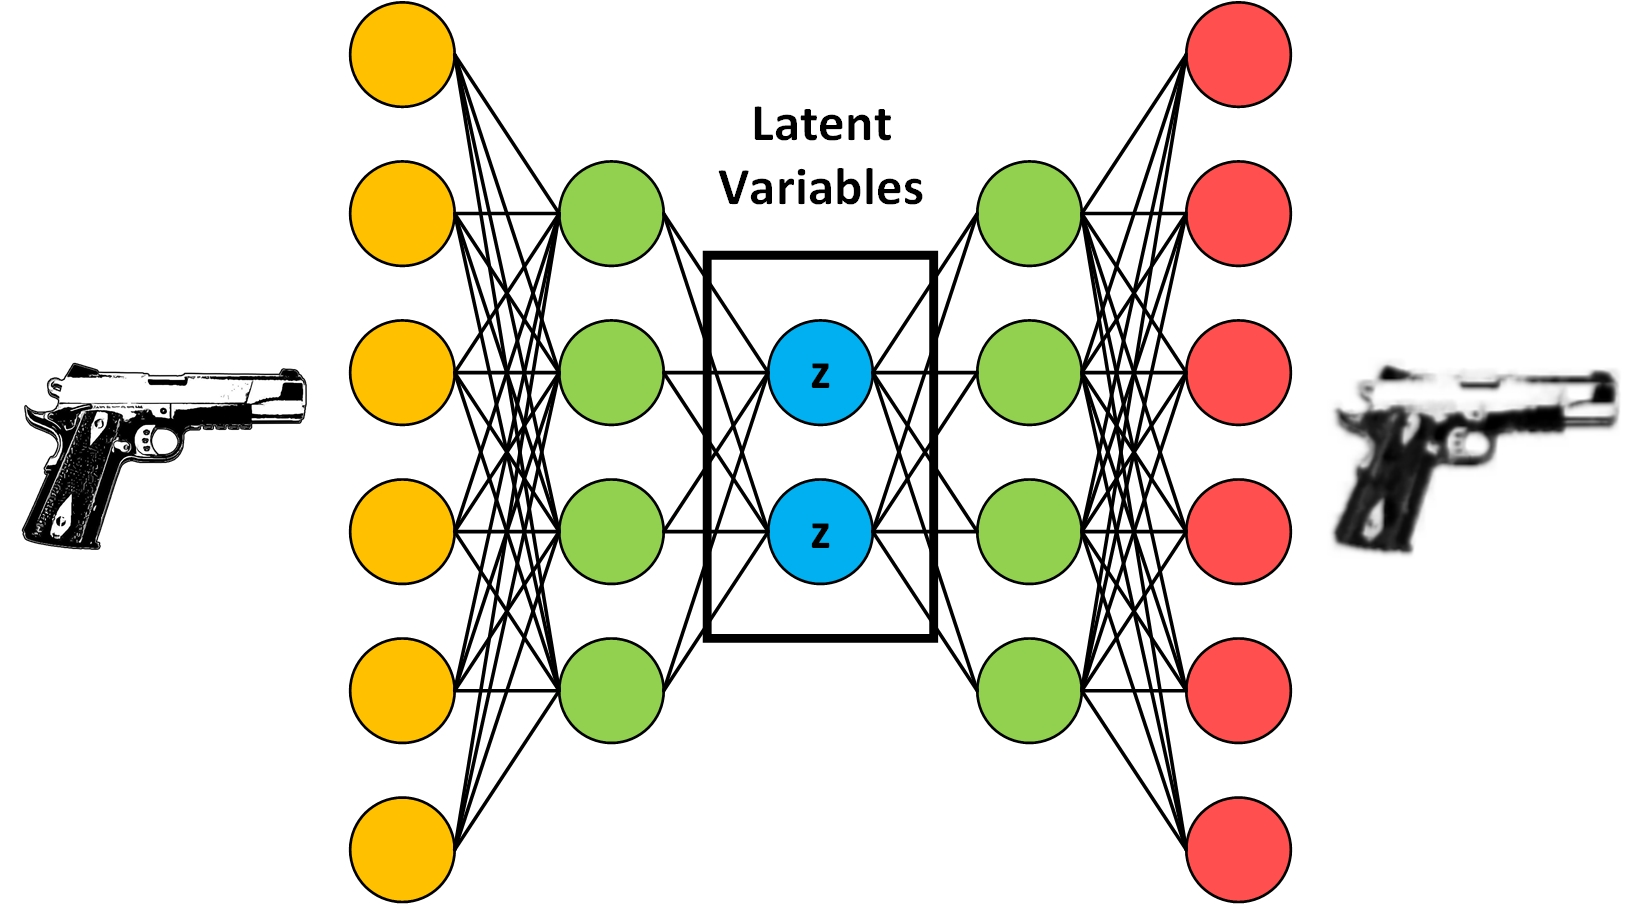
\includegraphics[width=0.9\linewidth]{PICs/NNs/autoencoder}
	\caption{Schematic representation of an autoencoder neural network with a blurry output.} \label{fig::autoencoder}
\end{figure}

The latent space got its name because someone does not necessarily know which features led to it \cite{ml::vae::tutorial}. It represents a transformed representation of the most valuable input data features. For example, someone could think of handwritten numbers and identify a latent variable in the number eight as the upper circle of the number. With this, the decoder would always reproduce this circle during decoding since it learned it as it would be a shared feature among all features. This assumption would make sense if there are only the same numbers in the input data but not if there are many different. Furthermore, if the latent space has the same dimension as the input or hidden space, then it could easily happen that all the information is fed straight forward through the network without any encoding, decoding and latent vector creation. This network constellation is the worst case and is not intended.\\
Now, the \ac{VAE} makes use of the same technique and resembles a traditional \ac{AE} \cite{ml::vae::tutorial}. The primary difference is that it alters the latent space with new variables and a sampling process to map the input data latent space onto a normal distribution like a Gaussian distribution instead to a fixed vector \cite{ml::vae::tutorial}. Figure \ref{fig::vae} shows a schematic representation of a VAE network and the difference to regular \acp{AE}. 
\begin{figure}[!htbp]
	\centering
	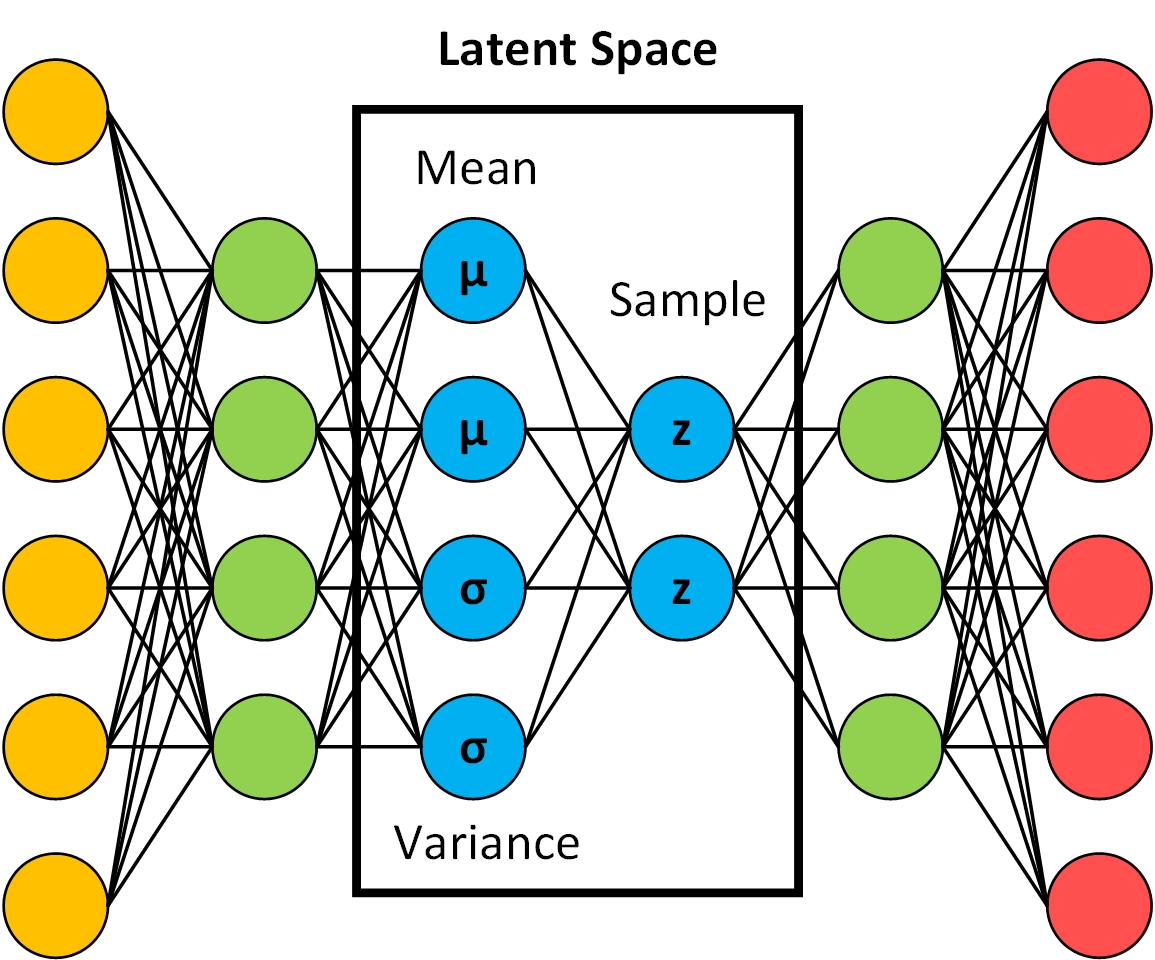
\includegraphics[width=0.65\linewidth]{PICs/NNs/variational_autoencoder}
	\caption{Schematic representation of a variational autoencoder neural network.} \label{fig::vae}
\end{figure}

It is worth noting, that all of the mentioned details of VAEs are excerpts from the excellent tutorial on VAEs from \citep{ml::vae::tutorial} which shall serve as a further reading source if the reader is interested in the detailed mathematics of VAEs.

Now, as seen in Figure \ref{fig::vae}, the VAE adds two new variables to the latent space. The variables $\mu$ and $\sigma^{2}$ represent the mean and variance of a normal distribution and are trained and learned via backpropagation and the so-called "reparameterization trick." The variable $z$ is the actual latent vector which is a combination of $\mu$, $\sigma^{2}$ and a random number sample $\varepsilon$ from a normal distribution. Now, the reparameterization trick introduces the random sample variable $\varepsilon$ which enables the possibility of backpropagation and helps to map the estimated distribution onto a normal distribution. In specific, the sampling process is applied to alter the latent vector and furthermore the output of the decoder network. However, the actual normal distribution mapping happens with the optimization part of the network which works as follows:
\begin{enumerate}
	\item Calculate the reconstruction loss of the decoded data compared to the real data.
	\item Calculate the so-called "Kullback-Leibler divergence" or short "KL-divergence" which makes sure that the latent vector $z$ stays close to a normal distribution with a mean of zero and a standard deviation of one.
	\item Combine the reconstruction loss and the KL-divergence to form the actual cost of the current training batch.
	\item Take the calculated overall cost and use backpropagation to optimize the model and minimize the cost.
\end{enumerate}

It is worth noting that only the variables $\mu$ and $\sigma^{2}$ are affected and adjusted by the backpropagation algorithm. The latent vector $z$ is omitted and acts as a helper vector for the sampling process. Otherwise, if $z$ would not exist, then it would create a barrier for the backpropagation algorithm since there would be a stochastic unit in the network \cite{ml::vae::tutorial}. For this reason, the random sample $\varepsilon$ acts as a new input layer and stochastic unit in the network which is applied to $z$ and not affected by backpropagation \cite{ml::vae::tutorial}. That means $z$ gets indirectly adjusted and optimized because it is a combination of $\mu$, $\sigma^{2}$, and the sample $\varepsilon$.

Furthermore, as the latent vector is always trained with a random normal distribution sample and mapped to a normal distribution, it enables the decoder to decode from noise data \cite{ml::vae::tutorial}. Figure \ref{fig::vae_noise_decoding} shows an example of this behavior where the decoder decodes noise data back to the learned data. 

\begin{figure}[!htbp]
	\centering
	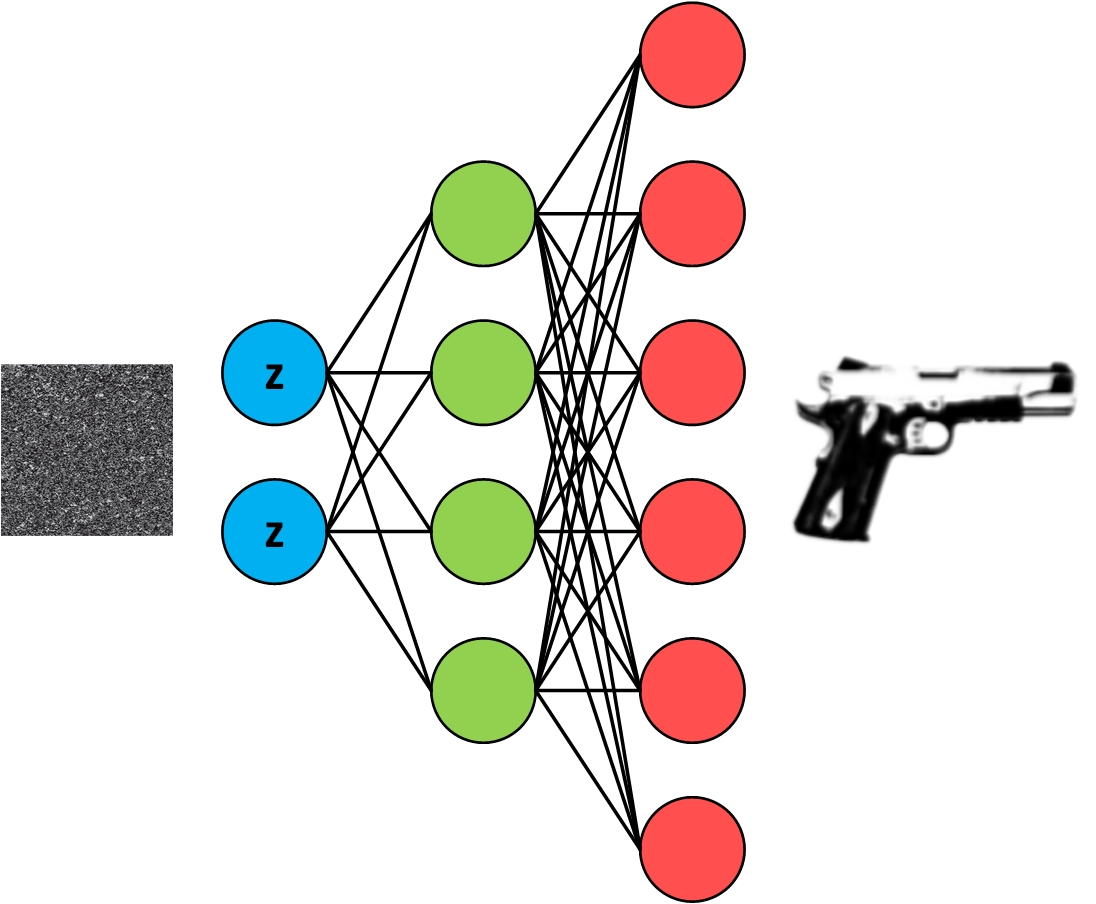
\includegraphics[width=0.7\linewidth]{PICs/NNs/variational_autoencoder_noise_decoding}
	\caption{Variational autoencoder latent space noise input decoding.} \label{fig::vae_noise_decoding}
\end{figure}

This possibility offers an excellent advantage for generating weapons from noise of a random normal distribution. In specific, the explanation for why this is even possible is easy to understand with the words of \citep[p. 6]{ml::vae::tutorial}: "Any distribution in $d$ dimensions can be generated by taking a set of $d$ variables that are normally distributed and mapping them through a sufficiently complicated function."

However, decoding from noise input is not the only advantage. Another advantage is that this also enables the usage of noisy input on the encoder side which means that one can add noise to the parameters of the input and the network will still generate a new weapon based on the data. 


%
% ------------------------------- NEW CHAPTER ------------------------------- %
%
\clearpage
\chapter{Prototype Development}
This chapter addresses every step of the development process of the weapon generator game mechanic but does not cover UE4 specific game development topics. All previously mentioned considerations apply to this implementation. It shows the development from the beginning to the end and sums it up with additional profiling plots for performance concerned readers. The ordering of all following chapters reflects more or less the actual workflow taken during the development. The prototype was implemented with Python version 3.6.4 and TF 1.8.0 in Jupyter Notebook and then integrated into UE4 4.19.2; the source code developed for the prototype is available on GitHub\footnote{\url{www.github.com/bernhardrieder/PCGML-Game-Mechanics}}. 

\section{Data Preprocessing} \label{dev::dataPreprocessing}
The first step of the development is the gathering and preprocessing of the \ac{BF1} community weapon analytic raw data. All of the weapon data is accessible to everyone via the community website of \citep{symthic::bf1stats}. The community of \citename{symthic::bf1stats} kindly provides a database dump on request which was extracted with a script by a community administrator. This database dump contains every parameter of the weapons in a readable and manageable way.

\subsection{Dump Extraction} \label{chapter::dumpExtraction}
More specifically, the dump contains 148 weapons with 90 parameters each. Some of the parameters can contain a list of further parameters. For example, the damage parameter consists of a collection of different damage values which are listed related to distances. For this reason, the damage and distance parameters were split into the first and last values to simplify the extraction and the weapon implementation. The full list of available parameters and their explanations is available in Appendix \ref{bf1::dumpParams}.

Now, it would be more than impracticable to manually extract the useful data out of the dump data file. The file has 13764 lines, and it would probably cause dozens of errors and wrong extractions. Therefore, the development of a simple Python script to extract all the data into a ".csv" file was the simplest way to achieve a consistent data extraction. 

The script reads a ".txt" file with the specified headers to extract in it as input and then extracts these specified header names from the dump file. Right after completing the data gathering process, it creates a new .csv file with a timestamp and adds the extracted data in an organized way so that someone can further process it by hand.

\subsection{Manual Dimension Reduction, Addenda and Unification}
One of the most significant issues in the extracted data was the ammo which was listed as it would be a different one for some weapons even if it is the same. For this reason, a manual examination of all ammo types was necessary to unify the range of all ammo types. 

\subsubsection{Weapon Type and Fire Modes}
It turned out that the dump does not include the specific types and fire modes of the weapons. Hence, it was necessary to examine that from the different game communities \citep{symthic::bf1stats}, \citep{bf1::community1}, and \citep{bf1::community2}. This proceeding added the unified weapon types of pistols, rifles, sniper rifles, shotguns, light machine guns and sub-machine guns as well as the unified fire modes of single-action, semi-automatic and automatic. Some of the weapons in \ac{BF1} have more fire modes available which were further simplified by the highest available fire mode. For instance, if a weapon can shoot with semi-automatic and automatic, then automatic was chosen. Besides, the game specifies more fire modes than the ones used. For example, they are using bolt-action, pump-action, single-barrel fire, and lever-action which were summarized as single-action weapons since they are using the same mechanic. Additionally, the weapons of BF1 have the possibility of double-action and double-barrel fire which is now a semi-automatic weapon in the dataset. Charts about the distribution of these two categories in the dataset are available in Appendix \ref{bf1::data::distributionCharts}. 

\subsubsection{Reload Times}
Another problem was caused by the reload times of the weapons because \ac{BF1} uses distinct reload mechanics for some weapons. In particular, the weapons of BF1 are from WW1 and weapons of this time do not always have the same magazines as used in modern weapons. Some of them do have special strip clip magazines instead of closed magazines which introduced  a particular reload mechanic. However, the community of \citep{symthic::bf1stats} provides an explanation to this reload mechanic which made a manual calculation and unification of the reload times for all magazine types possible so that there is no need of a distinction in the prototype implementation.

\subsubsection{Omitted Parameters and Final Set}
Table \ref{battlefield::weaponStats} shows some parameters which are not very useful for the training of the VAE which makes it necessary to omit some of these variables further. For example, the following parameters were omitted for specific reasons:
\begin{itemize}
	\item The bullet drop is almost the same for each weapon and would not have a big impact during the training.
	\item The ammo types would need encoding which could probably cause the curse of dimension since there are about 30 different used ammo types in the dataset.
	\item The reload time for ammo if some bullets are available in the magazine is more comfortable to handle if it is directly calculated from the reload time for an empty magazine.
	\item The last omitted parameter is the recoil in the left direction which showed that it is always the same value as the recoil in the right direction.
\end{itemize}

This refinement led the final set of parameters to the parameters shown in Table \ref{table::bf1::usedParams}. Note that the names of the parameters, except type and fire mode, are the same names as in the dump file provided by the \citename{symthic::bf1stats} community. Moreover, the damages and distances are listed as two parameters but are four parameters, as already mentioned in Chapter \ref{chapter::dumpExtraction}.
\begin{table}[!ht]
	\centering
	\begin{tabular}{|l|p{10.8cm}|}
		\hline
		\textbf{Parameter} & \textbf{Explanation} \\ \hline
		Type & The type of the weapon. \\ \hline
		FireMode & The fire mode of the weapon. \\ \hline
		Damages & Damage points applied, listed based on distance. \\ \hline
		Dmg\_distances & The distances in correlation to each damage entry in the "Damages" parameter. \\ \hline
		HIPRecoilDec & Weapon recoil decrease if the character is not aiming down sight. \\ \hline
		HIPRecoilRight & Weapon recoil upper bound of random recoil if the character is not aiming down sight. \\ \hline
		HIPRecoilUp & Weapon recoil upwards if the character is not aiming down sight. \\ \hline
		HIPStandBaseSpreadDec & The decrease of shot spread if the character is standing, not moving, and not aiming down sight. \\ \hline
		HIPStandBaseSpreadInc & The increase of shot spread if the character is standing, not moving, and not aiming down sight. \\ \hline
		InitialSpeed & Muzzle velocity. \\ \hline
		MagSize & Size of one magazine. \\ \hline
		ReloadEmpty & The time it takes if the magazine is empty. \\ \hline
		RoF & The rate of fire. \\ \hline
		ShotsPerShell & The number of pellets of one shot. \\ \hline
	\end{tabular}
	\caption{Used weapon parameters for the training of the \ac{VAE}.}
	\label{table::bf1::usedParams}
\end{table}

\subsection{Encoding and Feature Scaling}
The next part of the data preprocessing is the encoding and feature scaling task so that the VAE can efficiently process and train the network. 

\subsubsection{Encoding}
The first part is to encode the two only categorical parameters in the dataset. On this account, TF offers encoding mechanisms which help to encode the fire modes and weapon types. The encoding procedure is the same as demonstrated in Chapter \ref{ML::dataPreprocessing} and encodes the two categorical parameters into nine parameters. Therefore, the total number of features in the dataset after encoding is 23.

\subsubsection{Feature Scaling}
Now, the last part is to normalize or standardize all features. In particular, this is a necessary procedure for this dataset because there are many different value ranges. For example, the rate of fire and muzzle velocity are large numbers whereas the values of the spread increase or decrease are small. If there is no normalization or standardization, then this would cause significant extra expenses, as explained in Chapter \ref{chapter::ml::feature_scaling}.

The approach used for the dataset is the standardization process since it transforms the data in a way so that it has the properties of a standard distribution which may be useful during the \ac{VAE}'s training. 

\subsection{Training and Test Dataset}
The total dataset consists of 148 weapon constellations. A typical split of the data would be 80\% training data and 20\% test data. For this reason, the dataset split is a training set of 127 weapons and a test set of 21 entries which are about 16\%. The selection of the weapons for the test set was done randomly and took into account to include at least as many weapons as different fire modes, and weapon types are available, as well as different weapons with values in low, middle and high range for damage, rate of fire, muzzle velocity, magazine size and reload time.

\subsection{Convenience Class Overview}
TF offers many tutorials on how to use and develop with TF. A standard dataset used in the tutorials is the MNIST dataset which encapsulates its data into a convenience class. This class served as a base and inspiration for an own convenience class which encapsulates the weapon data. Following Listing \ref{pseudoCode::weponDataSet} presents the most valuable functions and accessible members of this convenience class:

\begin{lstlisting}[language=,name={Essential functions and properties of the weapon dataset convenience class.},label={pseudoCode::weponDataSet}]
global functions:
	get training and test data
	
class DataSet:
	properties:
		standardized and encoded data
		number of features in data
		number of data examples
		standardized minimum values
		standardized maximum values 
	functions:
		get next batch for training either shuffled or not
		add new weapons to the dataset
		re-standardize the whole data
		encode and standardize features
		decode a processed tensor from TensorFlow
		encode decoded tensor from TensorFlow
\end{lstlisting}

\section{\acl{VAE}}
The implementation of the \ac{VAE} was driven and inspired by the explanation of \citep{tutorial::vaeTF}. \citename{tutorial::vaeTF} used a high-level approach in his design which is similar to high-level \ac{ML} \acp{API}. These high-level \acp{API} are easily modifiable and extensible which was the main reason for following this approach. An easy modification is necessary to test different network hyperparameters without significant changes in the code and thus to find the most suitable network parameters. In particular, Chapter \ref{chapter::vae::network} explains the entire proceeding of the hyperparameters selection process. Now, the next chapters show an overview of the \ac{VAE} class, how the model accuracy was measured to obtain an adequately trained model, address the already mentioned network parameter selection, show two weapon generation examples and list development issues.

\subsection{Class Overview}
Listing \ref{pseudoCode::vae} shows a \ac{VAE} class overview with most of the available and necessary functions for the generation task. The actual code contains some more functions which are not essential to explain. As already introduced in the weapon convenience class, this class also has some global convenience functions to obtain different stages of a \ac{VAE}. 

Two of the most essential functions of the \ac{VAE} class for the weapon generation tasks are the functions "decode from latent space" and "encoding and decoding" since they provide the functionality to generate data similar to the training data. It is to mention that the \ac{VAE} initializes itself on construction where it calls all the initialization functions to maintain a working network. The last most important function to mention is the loss calculation function since it is necessary to secure a working generation during generation time so that the weapon is actually from the distribution of the network and that the network was able to recreate a weapon from that distribution.

\begin{lstlisting}[language=,name={Essential functions of the VAE class.},label={pseudoCode::vae}]
global functions:
	get an untrained variational autoencoder
	get a fully trained variational autoencoder
	
class VariationalAutoencoder:
	public functions:
		train the model with a batch
		decode a batch from latent space
		encode and decode a batch
		load the trained model from file
		save the trained model to file
		calculate the loss from a batch
	private functions:
		create the encoder network
		create the z sampling operation
		create the decoder network
		create a hidden layer
		create the weights and biases
		create the loss optimizer
		calculate the reconstruction loss
		calculate the Kullback-Leibler divergence
\end{lstlisting}

\subsection{Model Accuracy Measurement}
One of the most important parts of training the VAE is to secure a high model accuracy. Two different measurements will secure this accuracy:
\begin{itemize}
	\item The value of the test set reconstruction loss.
	\item The value of a random input reconstruction loss.
\end{itemize} 
Now, as already mentioned in Chapter \ref{dev::dataPreprocessing}, the data was split into 127 weapons as training data and 21 weapons as test data. Both of the inputs are feed into the encoder side of the network which outputs the manually examined test results. Following steps were taken to ensure a high model accuracy:
\begin{enumerate}
	\item Measure the model reconstruction accuracy by calculating the average loss caused by the test set.
	\item Generate a random input in the range of the normalized values of the test set and size of the test set and measure the caused average loss.
	\item Make sure that the average reconstruction loss of the test set is as small as possible and the loss of the random input is as massive as possible.
\end{enumerate}
Now, if the random input loss is very high, then it means that the model has learned the internal structure and dependencies of the training data because it cannot classify the input data regarding the training data. In other words, a significant loss with random input data means that the model has no idea which data is that supposed to be and cannot reconstruct anything useful. On the other hand, if the reconstruction loss of the test set would be very high, then it would not know what to reconstruct either. Therefore, it is crucial to secure a low loss with the test set and a high loss of the random input.

\subsection{Network Hyperparameter Selection} \label{chapter::vae::network}
Finding the right network hyperparameters for a \ac{NN} seems to be one of the trickiest parts in designing a \ac{NN}. Different constellations of learning rate, optimizer function, hidden layer size, latent space size, number of training data features, activation functions after the hidden layers, batch size and training epochs can have similar, better or worse performance since the weights and biases in the \ac{NN} are randomly initialized, dynamically trained and can emerge in either the right or wrong way. For this reason, the development of a simple hyperparameter test script was the easiest way to tackle that problem and detect the most promising parameters. This test script iterates over each possible constellation and measures the average loss of an entire test set. However, before any of the test iterations were in progress, the assumptions for a properly working network were evaluated as follows:
\begin{itemize}
	\item \textbf{Learning rate}: Between 0.01 and 0.001 because the weapon variables are standardized and bigger rates would not make sense.
	\item \textbf{Size of the hidden layers}: Bigger than the latent space but smaller than the input layer size to prevent the straightforward passing on of the variables without any training of the weights.
	\item \textbf{Size of the latent space}: Not smaller than two and not bigger than the hidden layer because of the same reason as mentioned in the hidden layer.
	\item \textbf{Activation function after hidden layers}: The commonly used hyperbolic tangent activation function  "tanh" which outputs values between -1 and 1. 
	\item \textbf{Optimizer function}: The common optimizer function "Adam" \cite{ml::optimizer::overview}.
	\item \textbf{Batch size}: Not larger than ten because of the small amount of training data.
	\item \textbf{The number of training epochs}: Inestimable but probably not more than 500.
\end{itemize}
However, after some test iterations, the values to all the hyperparameters were set empirically, as those that achieved the best performance in the application domain.
\begin{itemize}
	\item \textbf{Learning rate}: 0.01.
	\item \textbf{Size of the hidden layers}: 26 neurons in the first hidden layer and 12 in the second hidden layer.
	\item \textbf{Size of the latent space}: 2 neurons.
	\item \textbf{Activation function after hidden layers}: The exponential linear unit activation function "elu" which leads to higher classification accuracies \cite{ml::activation::elu}.
	\item \textbf{Optimizer function}: The optimizer function "RMSProp" \cite{ml::optimizer::overview}.
	\item \textbf{Batch size}: 4.
	\item \textbf{The number of training epochs}: A number of 400 shows the lowest costs. 
\end{itemize}
It was interesting to see that the exponential linear unit activation function was able to detect the underlying structure of the data much better than the standard hyperbolic tangent activation function. This detection was then further boosted with a collaboration with the RMSProp optimizer. Why these particular activation function and optimizer works so good would be interesting to know but exceed the scope of this thesis and therefore is not addressed.

\subsubsection{Latent Space Visualization}
A lucky coincidence of these hyperparameters is that the latent space has a dimension of two neurons which means that it is easy to illustrate the values in the latent space. For this reason, Figure \ref{fig::vae::untrainedLatentSpace} shows the parameter $\mu$ of an untrained latent space and Figure \ref{fig::vae::trainedLatentSpace} shows the parameter $\mu$ of a trained latent space after 70 epochs. The left side of the figure shows one dot per weapon whereas the right side shows the same as the left side but with a density per dot.
\begin{figure}[!ht]
	\centering
	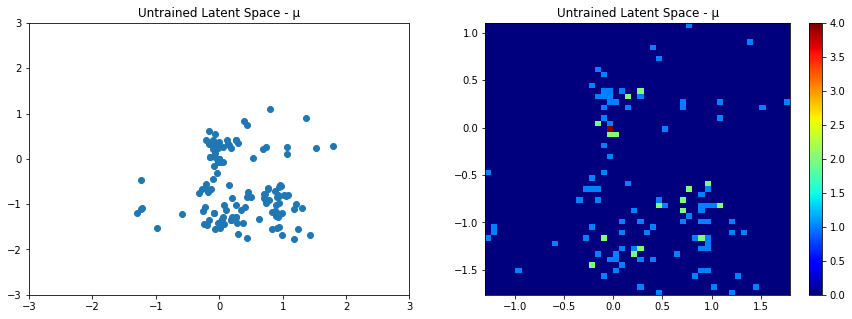
\includegraphics[width=1.0\linewidth]{PICs/trained_vae/untrained_latent_space}
	\caption{Visualization of the untrained latent space.} \label{fig::vae::untrainedLatentSpace}
\end{figure}
\begin{figure}[!ht]
	\centering
	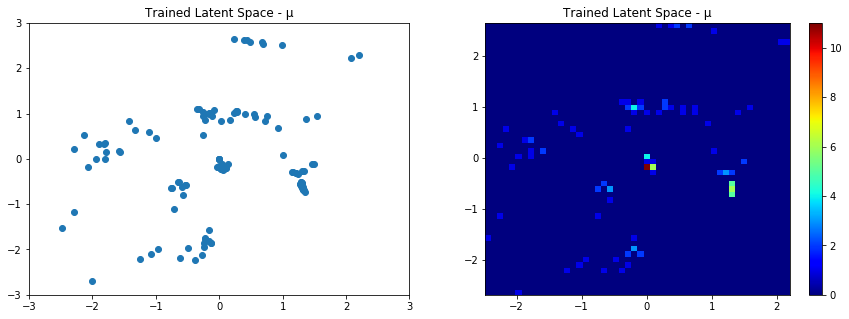
\includegraphics[width=1.0\linewidth]{PICs/trained_vae/trained_latent_space}
	\caption{The trained latent space after 70 training epochs.} \label{fig::vae::trainedLatentSpace}
\end{figure}

Looking at Figure \ref{fig::vae::trainedLatentSpace}, one can easily see that the model was able to learn an underlying structure of the provided weapon data. Furthermore, someone can easily assume and connect the six visible clusters in the plot to the available weapon types in the training data.

\subsubsection{Cost per Training Epoch}
Another chart which helps to determine the right amount of training epochs shows Figure \ref{fig::vae::costPerEpoch}. This chart shows that there is a minimum average cost at around 400 to 1000 training epochs which will slightly rise with more and more epochs. This chart contains the average costs of 50 observations with 20 percent outliers included.
\begin{figure}[!ht]
	\centering
	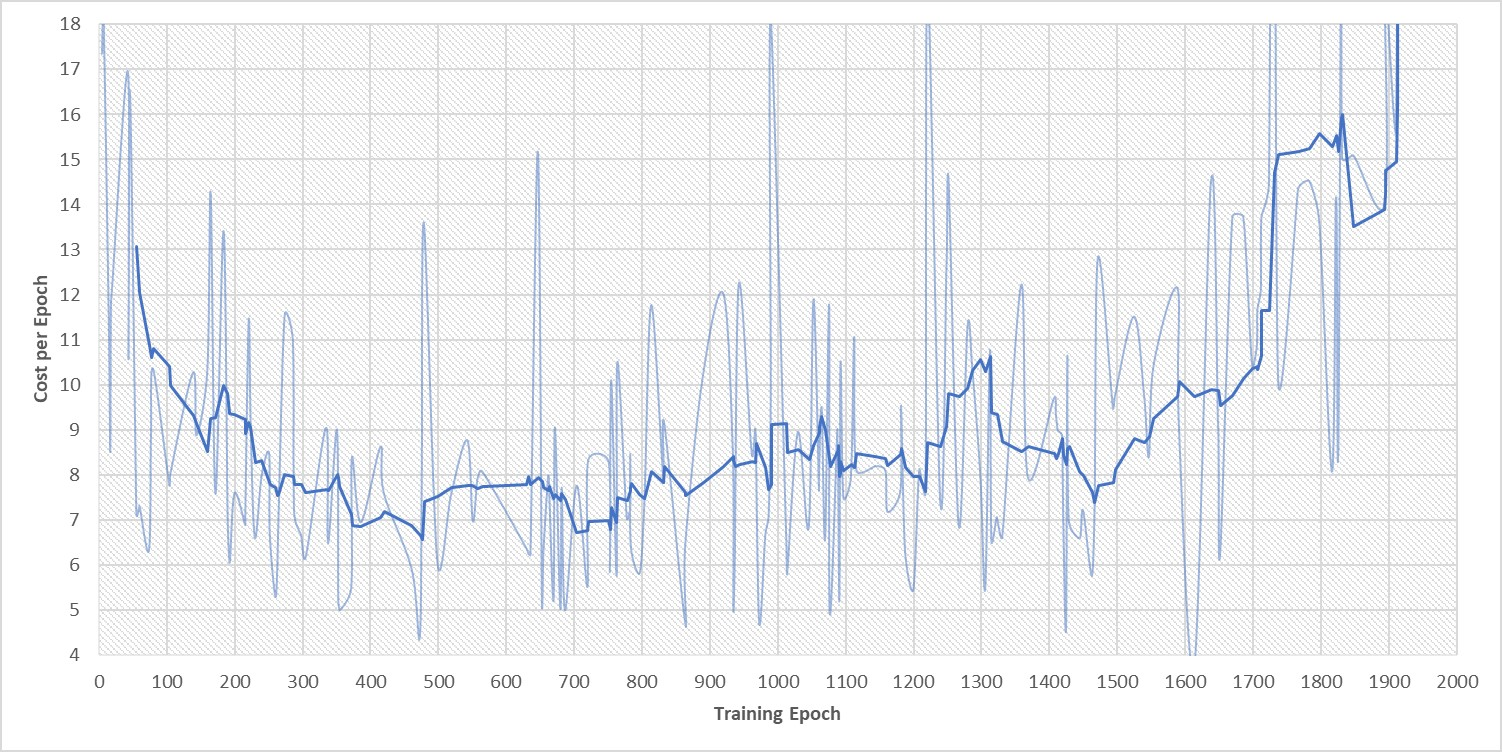
\includegraphics[width=1.0\linewidth]{PICs/trained_vae/cost_per_epoch}
	\caption{The average cost per training epoch of 50 observations.} \label{fig::vae::costPerEpoch}
\end{figure}

\subsubsection{Test Data Sample versus Random Sample Input}
Another benchmark to determine the right amount of training epochs is to compare the test results of the network with the different input of random sample and test data sample input. Figure \ref{fig::vae::epochsFailureRate} shows this comparison in a chart with separate lines for each input. Each observation point in the chart was calculated with the average of 25 observations and includes 20 percent of outliers. Calculated cost values over 1000 or the ones not identified as number were clamped to 1000. Furthermore, please take note, that this samples are inputted into the encoder and that a small average cost indicates a successful recreation of the input. Therefore, Figure \ref{fig::vae::epochsFailureRate} perfectly demonstrates that the network does not know what to do with random sample input.
\begin{figure}[!ht]
	\centering
	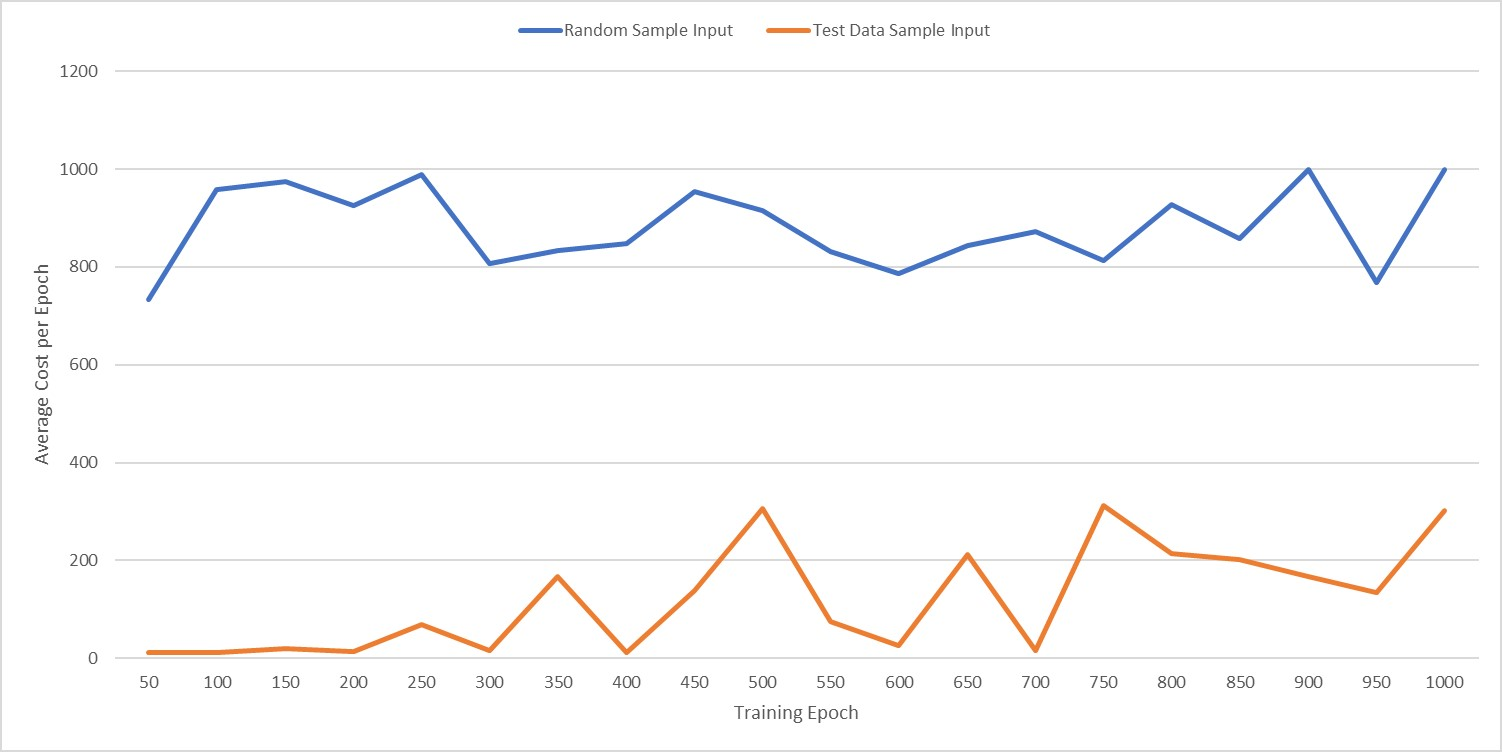
\includegraphics[width=1.0\linewidth]{PICs/trained_vae/epoch_failure_rate}
	\caption{A comparison of the average costs of random sample versus test data sample input.} \label{fig::vae::epochsFailureRate}
\end{figure}

Now, an examination of the comparison chart shows that the average costs or rather losses for the test dataset starts to fluctuate with more and more training epochs whereas the the average cost for a random input sample remains high. Hence, the decision for the training epochs in the weapon generation was set to 70 epochs in the beginning and will increase with every newly added weapon to the dataset. 

\subsection{Random Input Generation Example} \label{vae::randomInputExample}
Table \ref{vae::randomInputGeneration} shows a comparison of a training weapon and a weapon which was generated with random noise input to prove that the trained \ac{VAE} can generate useful weapon data. One can see that the \ac{VAE} has issues with predicting and generating the correct category for a weapon. This issue is still an unsolved problem but is easily solvable by checking the highest value of all categories. In this case, it is most likely a sniper rifle with semi-automatic fire mode. Please note that the listed parameters are the same parameters which are outputted by the \ac{VAE}.
\begin{table}[!ht]
	\centering
	\begin{tabular}{|l|p{3.6cm}|p{3.6cm}|}
		\hline
		\textbf{Output Parameter}       & \textbf{Training Weapon} & \textbf{Random Generated Weapon} \\ \hline\hline
		damages\_first           & 26.5                 & 42.767                    \\ \hline
		damages\_last            & 6.25                 & 30.294                    \\ \hline
		distances\_first    & 14.0                 & 13.988                    \\ \hline
		distances\_last     & 21.0                 & 60.002                    \\ \hline
		firemode\_Automatic      & 0.0                  & 0.302                     \\ \hline
		firemode\_Semi & 0.0                  & 0.333                     \\ \hline
		firemode\_Single & 0.0                  & 0.234                     \\ \hline
		hiprecoildec             & 6.0                  & 5.183                     \\ \hline
		hiprecoilright           & 1.2                  & 0.554                     \\ \hline
		hiprecoilup              & 11.0                 & 2.436                     \\ \hline
		hipstandbasespreaddec    & 4.5                  & 6.511                     \\ \hline
		hipstandbasespreadinc    & 0.3                  & 0.323                     \\ \hline
		initialspeed             & 333                  & 559.643                   \\ \hline
		magsize                  & 2                    & 20.258                    \\ \hline
		reloadempty              & 5.333                & 3.702                     \\ \hline
		rof                      & 299                  & 298.027                   \\ \hline
		shotspershell            & 12                   & 1.527                     \\ \hline
		type\_Pistol             & 0.0                  & 0.167                     \\ \hline
		type\_Rifle              & 0.0                  & 0.189                     \\ \hline
		type\_Shotgun            & 1.0                  & 0.067                     \\ \hline
		type\_Sniper       & 0.0                  & 0.189                     \\ \hline
		type\_SMG     & 0.0                  & 0.088                     \\ \hline
		type\_MG     & 0.0                  & 0.095                     \\ \hline
	\end{tabular}
	\caption{Comparison of a training weapon and a generated weapon with random noise as input.}
	\label{vae::randomInputGeneration}
\end{table}

\subsection{Development Issues}
Two particular issues occurred during the development with TF:
\begin{enumerate}
	\item It needs so-called sessions in TF to run TF operations. With the creation of this session is a so-called graph included which contains all network nodes and there will be no graph cleanup at session termination. In case of the necessary retraining for this network, this missing cleanup created massive pollution of the graph which slowed the execution bit by bit. The solution to this problem is a simple reset of the graph after the session termination and right before the new trained model update procedure.
	\item TF works with nodes which have a specific shape. If the node has no specific shape at creation time, then it will get one during the training, and will consist in the trained and saved model. For this reason, all of the network nodes will have a similar shape as the batch size because it propagates itself through every node in the network during the training. That means that encoding and decoding as well as simple decoding from latent space is just possible with an input which has the same size as the training batch. Of course, this is not a big problem but narrows the possibilities of using the \ac{VAE}. This problem was solved with a simple replication of the input if it is not the same size as the batch size and mean calculation of the output. For example, if the batch size is four, then it will generate four different weapons of the replicated input and returns the mean values of the generated weapons.
\end{enumerate}

\section{Game Scenario}
The prototype scenario was implemented in \ac{UE4} version 4.19.2 and includes a simple map with all requested elements described in Chapter \ref{chapter::gamePrototype}. Figure \ref{scenarioMap} shows the created map of the scenario from a top-down view, the possible spawn points of the player in green and the location of the end boss \ac{AI} in red. All \ac{3D} models and assets are either reused from \ac{UE4} template projects or were freely downloaded from the internet and do not violate any copyrights.
\begin{figure}[!ht]
	\centering
	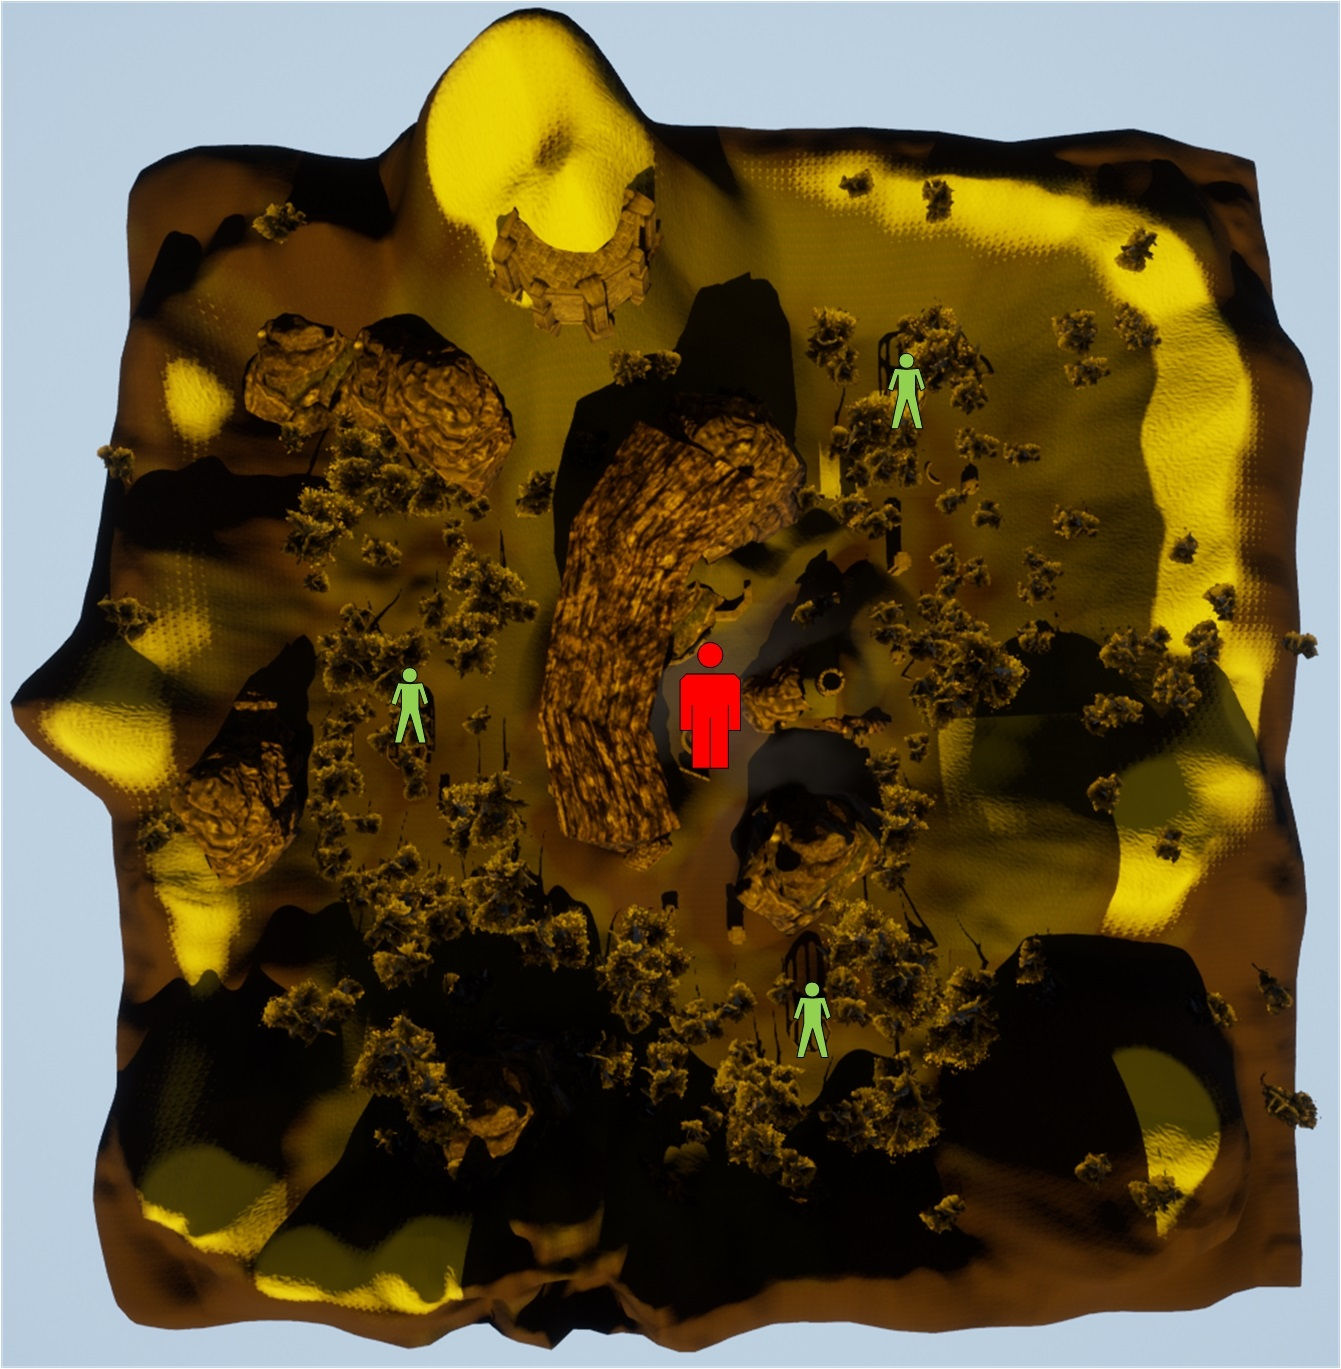
\includegraphics[width=0.6\linewidth]{PICs/Prototype/map_with_spawnpoints_and_boss}
	\caption{Prototype scenario map with player spawn points in green and boss in red.} \label{scenarioMap}
\end{figure}

Furthermore, Figure \ref{scenarioScreenshot} shows an in-game screenshot from the player's perspective with the \ac{HUD}, an enemy \ac{AI} with a health bar over the head and the waiting end boss \ac{AI}.
\begin{figure}[!ht]
	\centering
	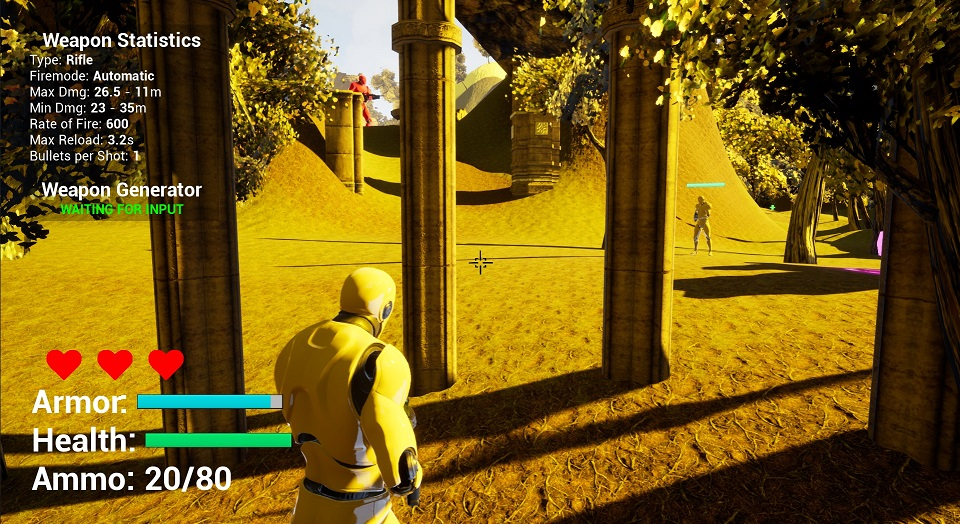
\includegraphics[width=1.0\linewidth]{PICs/Prototype/ingame_screenshot_small}
	\caption{Prototype scenario in-game screenshot.} \label{scenarioScreenshot}
\end{figure}

\subsection{\acl{HUD}}
As designed in Chapter \ref{chapter::gamePrototype}, the \ac{HUD} should provide the player with feedback to the mechanic and also the game. For this reason, it shows the most critical parameters of the currently equipped weapon on the top left, as visible in Figure \ref{scenarioScreenshot}. Furthermore, it shows the current status of the weapon generator which range from "Starting" to "Waiting for Input" to "Generating." The status of the available ammo, current health and armor, and lives is also shown in the \ac{HUD} so that the player knows about the vitals.

\subsection{Player}
The player can do everything as in common \ac{FPS} games and additionally has the possibility of using the weapon generator to generate a new weapon. If the player decides to dismantle the equipped weapon, then the currently equipped weapon will be removed from the player and the player can only use the remaining weapon until the generation is complete. Specific movement types increase or decrease weapon shooting behavior. Besides, the player can gather power-ups which are placed randomly on the map and increase or refill movement speed, health, armor, and ammo.

\subsection{Bots}
The implementation of the bots comes in three different types. The easiest one is a simple ball bot which moves towards the player and explodes some time after reaching the player. The two other bots are from the same type  which is visible in Figure \ref{scenarioScreenshot}, they move towards the player and shoot him or her with different weapons in a straightforward way. The easy bot does not cause much damage but tries to heal itself if the health is low whereas the difficult bot causes more damage, has more health and does not heal itself.

The end boss bot is even harder than the difficult bot and has an own weapon which has a higher rate of fire than any other weapons of the bots. Furthermore, the end boss has many health points so that the player needs to use the weapon generator to win against the boss.

\subsection{Weapons}
The weapon class contains almost every feature shown in Table \ref{table::bf1::usedParams}. The only omitted parameter is the initial speed or also known as muzzle velocity. For generator reasons, this parameter needs to be saved in the weapon class but does not affect the weapon since they are all working as ray-tracing weapons with instant hits. For further simplicity in the prototype, one class functions as a superclass for all different weapon types. Furthermore, to have a visible representation of the weapon, every weapon type has its weapon model so that the player can distinguish between the weapons inside the game. 

Moreover, each weapon has specific modifier which affects either the weapons or the player. For example, machine guns are heavier than pistols and therefore lower the movement speed of a character. Alternatively, if a player aims down sight, then the shooting behavior regarding recoil and spread is improved. These improvements can be adjusted for each weapon class and propagate to the generated weapons of the same weapon type.

\section{Weapon Generator}
As already mentioned at the beginning of this chapter, the weapon generator was implemented outside \ac{UE4} and imported as soon as it worked. Listing \ref{pseudoCode::weaponGeneratorAPI} shows the essential functions of the weapon generator \ac{API} class which inherits the functions from the \ac{TF} plugin \ac{API} class, described in Chapter \ref{whichGameEngine}. 
\begin{lstlisting}[language=,name={Essential functions of the TF plugin weapon generator API class.},label={pseudoCode::weaponGeneratorAPI}]
class WeaponGeneratorAPI:
	functions:
		on setup:
			initialize the network
		on begin training:
			train the model
		on json input:
			check if a new trained model is available
			add a dismantled weapon to the dataset and retrain the network if necessary
			process the input and return a new generated weapon
\end{lstlisting}

\subsection{Workflow}
The beginning of the game scenario directly triggers the initialization of the weapon generator as well as the setup and training of the \ac{VAE} model. This training runs on an own background thread so that the player does not notice the training at all at runtime. That is the moment in which the \ac{HUD} displays the status "Starting" as feedback of the generator for the player. Figure \ref{figure::weaponGen::init} shows the workflow of the weapon generator initialization.
\begin{figure}[!ht]
	\centering
	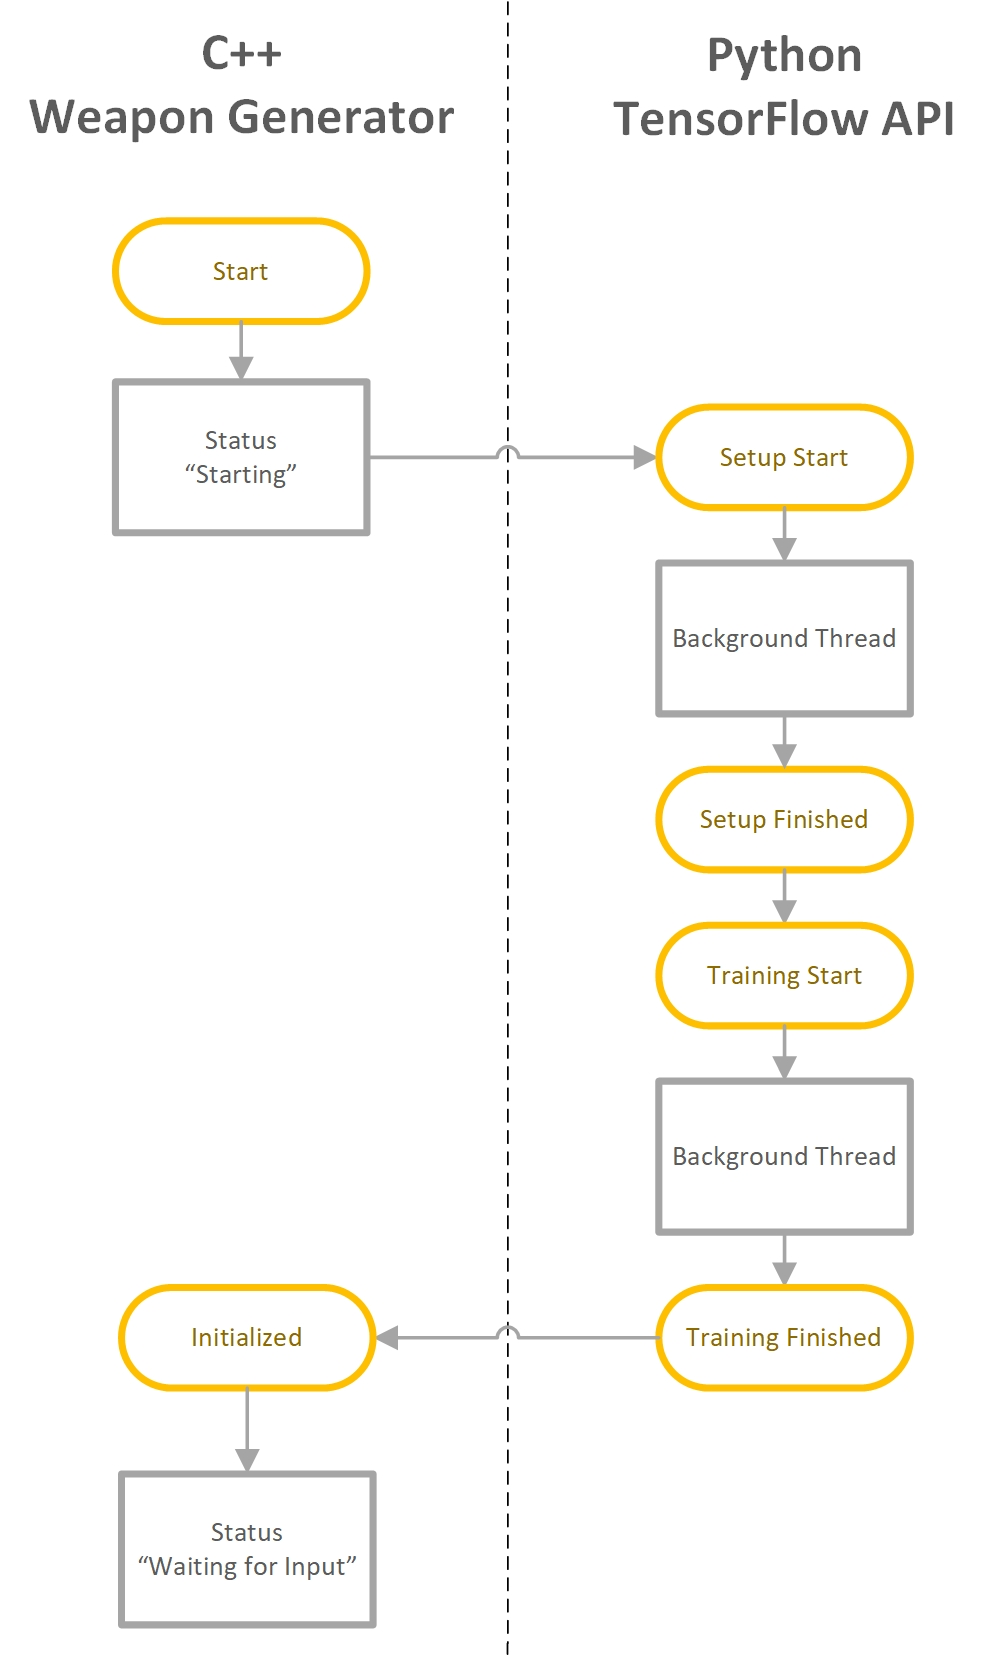
\includegraphics[width=0.5\linewidth]{PICs/WeaponGeneratorWorkflow_Setup_Training}
	\caption{Weapon generator setup and training workflow.} \label{figure::weaponGen::init}
\end{figure}\\
As soon as the generator has changed the status to "Waiting for Input," it is ready to use for the player. The player can now dismantle the equipped weapon which sends it to the weapon generator. Subsequently, the generator extracts all parameters of the weapon, applies some modification based on statistics, creates a \ac{JSON} formatted string and sends it to the Python \ac{API}. The applied statistics are the kills and used time of the weapon which changes the random change range of the parameters. The strength of each parameter and the starting range of the random change rate are adjustable parameters. A detailed description on how this operates is described in the next chapter. Figure \ref{figure::weaponGen::gen} shows the workflow of the dismantling process for generating a new weapon. Note that the generation process in the \ac{API} runs on a background thread so that the game does not freeze during that proceeding.
\begin{figure}[!ht]
	\centering
	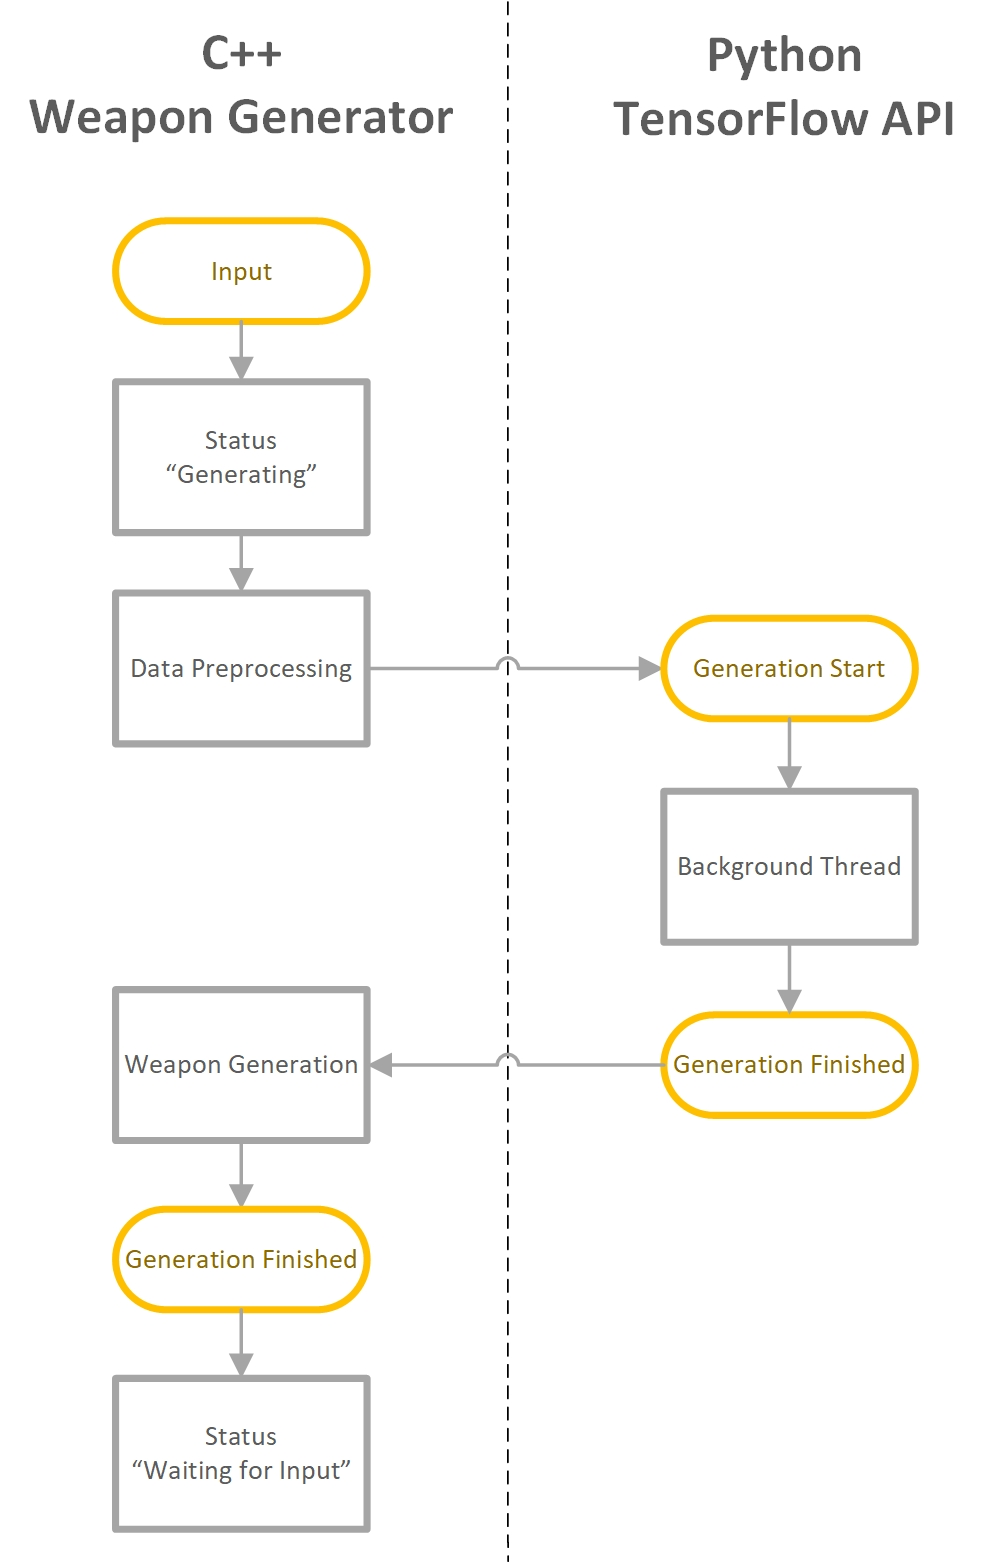
\includegraphics[width=0.5\linewidth]{PICs/WeaponGeneratorWorkflow_Generation}
	\caption{Weapon generator generation workflow.} \label{figure::weaponGen::gen}
\end{figure}\\
The generator changes the status to "Generating" during the processing of the dismantled weapon and the generation of the new weapon. Sometimes, this can take more time because of the retraining of the model, triggered after a specific amount of dismantled weapons. The generator creates either a weapon based on the statistics of the dismantled weapon or a random weapon if the average reconstruction costs exceed a specific threshold or a not unprocessable number.

As soon as the \ac{VAE} generator \ac{API} is ready and has sent the result back to the weapon generator, it creates a new weapon and notifies the player about the completion. Subsequently, the generator changes the status to "Waiting for Input" and can receive a new dismantled weapon. During the creation process of the new weapon, the generator checks and makes sure, that all of the parameters do not exceed critical values which could cause bugs in the game. 

\subsection{Parameter Modification and Adjustable Parameters}
As already mentioned, the parameters of the dismantled weapon are modified before sent to the generator \ac{API} which includes some adjustable parameter. The parameters of weapons are either increased or decreased depending on whether it would help the player against the boss. For example, the damage is increased whereas reload time is decreased and so forth. Now, the change of parameters results according to a random change rate which can be offset with kills or using time. The starting range and the strength of the kills and time are adjustable in the weapon generator. 

Other adjustable parameters are tolerance values which can add a random element to the weapon type and fire mode selection. The problem tackled with this proceeding was mentioned in Chapter \ref{vae::randomInputExample}. The \ac{VAE} sometimes generates small numbers which are almost similar to each other for every categorical parameter. The solution to this problem is first to obtain the highest value among the received values and then check which of the values lie in the specified tolerance range, based on the highest found value. Therefore, this tolerance causes a random selection among almost similar weapon types or fire modes.

\subsection{\acl{TF} Plugin Changes}
The default \ac{TF} version of the plugin is version 1.6.0. Nonetheless, the prototype development used version 1.8.0. For this reason, the version of \ac{TF} in the plugin was changed to 1.8.0 which could be done without any issues since the plugin is not dependent on any \ac{TF} specific variables.

The other significant change in the plugin was a change in the \ac{API} class which does not use a background thread for the input processing by default. This missing feature is causing a game freeze during the weapon generation and is not tolerable. This freeze will also happen if multithreading is disabled in the plugin which is not advisable. Therefore, the \ac{API} code was changed to run the input processing on a background thread and notify the \ac{API} on completion so that it can propagate the result to the weapon generator.

\section{Performance and Profiling}
Profiling was done in the \ac{UE4} Editor in development configuration with the following test device specifications:
\begin{itemize}
	\item \textbf{Product}: MSI GS60 2PE Ghost Pro
	\item \textbf{\ac{OS}}: Windows 10 64-bit
	\item \textbf{\ac{CPU}}: Intel Core i7-4710HQ CPU @ 2.50GHz
	\item \textbf{\ac{GPU}}: NVIDIA GeForce GTX 870M
	\item \textbf{\ac{RAM}}: 16GB
\end{itemize}

All of the following profiling charts are obtained with the same testing scenario. The scenario map is loaded, the weapon generator either initializes nor not, depending on its availability, and the game was then actively played for more than 30 seconds. Hence, the weapon generator was constantly used if available in the specific testing environment. 

Figure \ref{scenario::profiling_noTF} shows a profiling chart of the scenario map without any weapon generation mechanic enabled. The \ac{TF} plugin, its dependent Python plugin, and the SocketIO plugin were fully deactivated and did not affect the engine’s performance.
\begin{figure}[!ht]
	\centering
	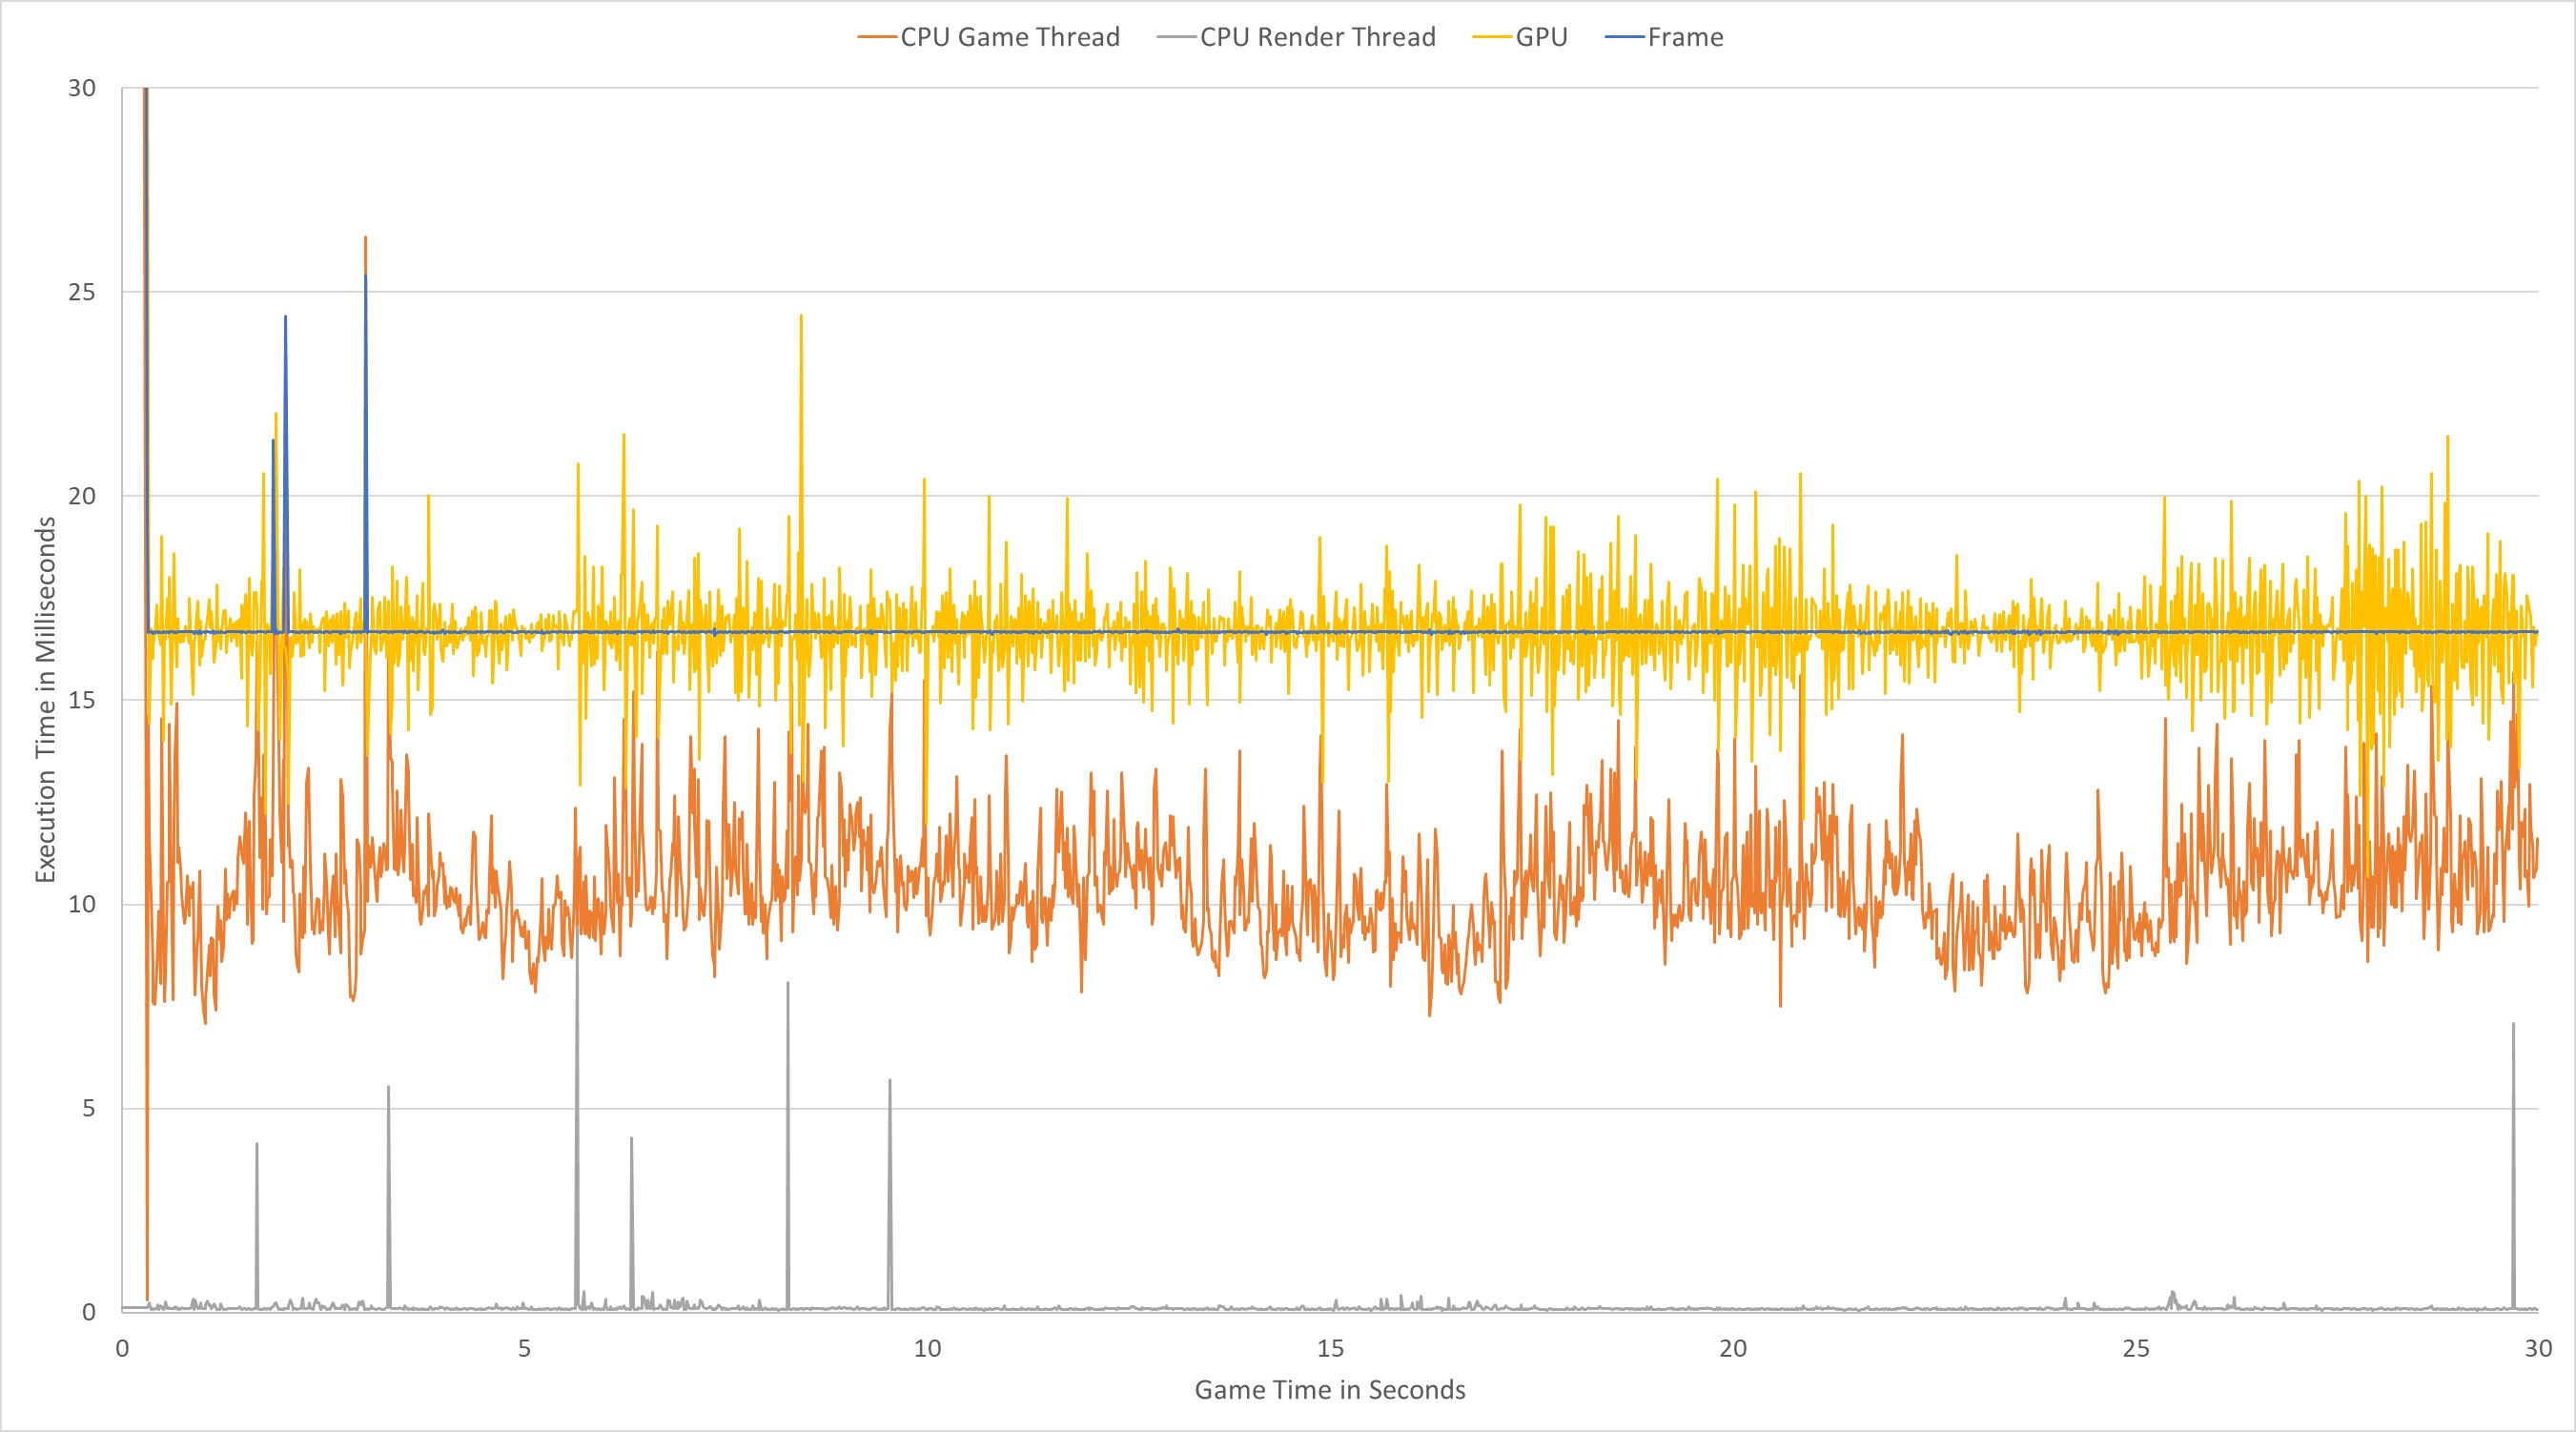
\includegraphics[width=1.0\linewidth]{PICs/Profiling/deactivated_plugin}
	\caption{Profiling chart with the deactivated TensorFlow Plugin.} \label{scenario::profiling_noTF}
\end{figure}

Figure \ref{scenario::profiling_TF} shows a profiling chart with an enabled \ac{TF} plugin but which was not actively used in the game. Therefore, the weapon generator was not available for the player.
\begin{figure}[!ht]
	\centering
	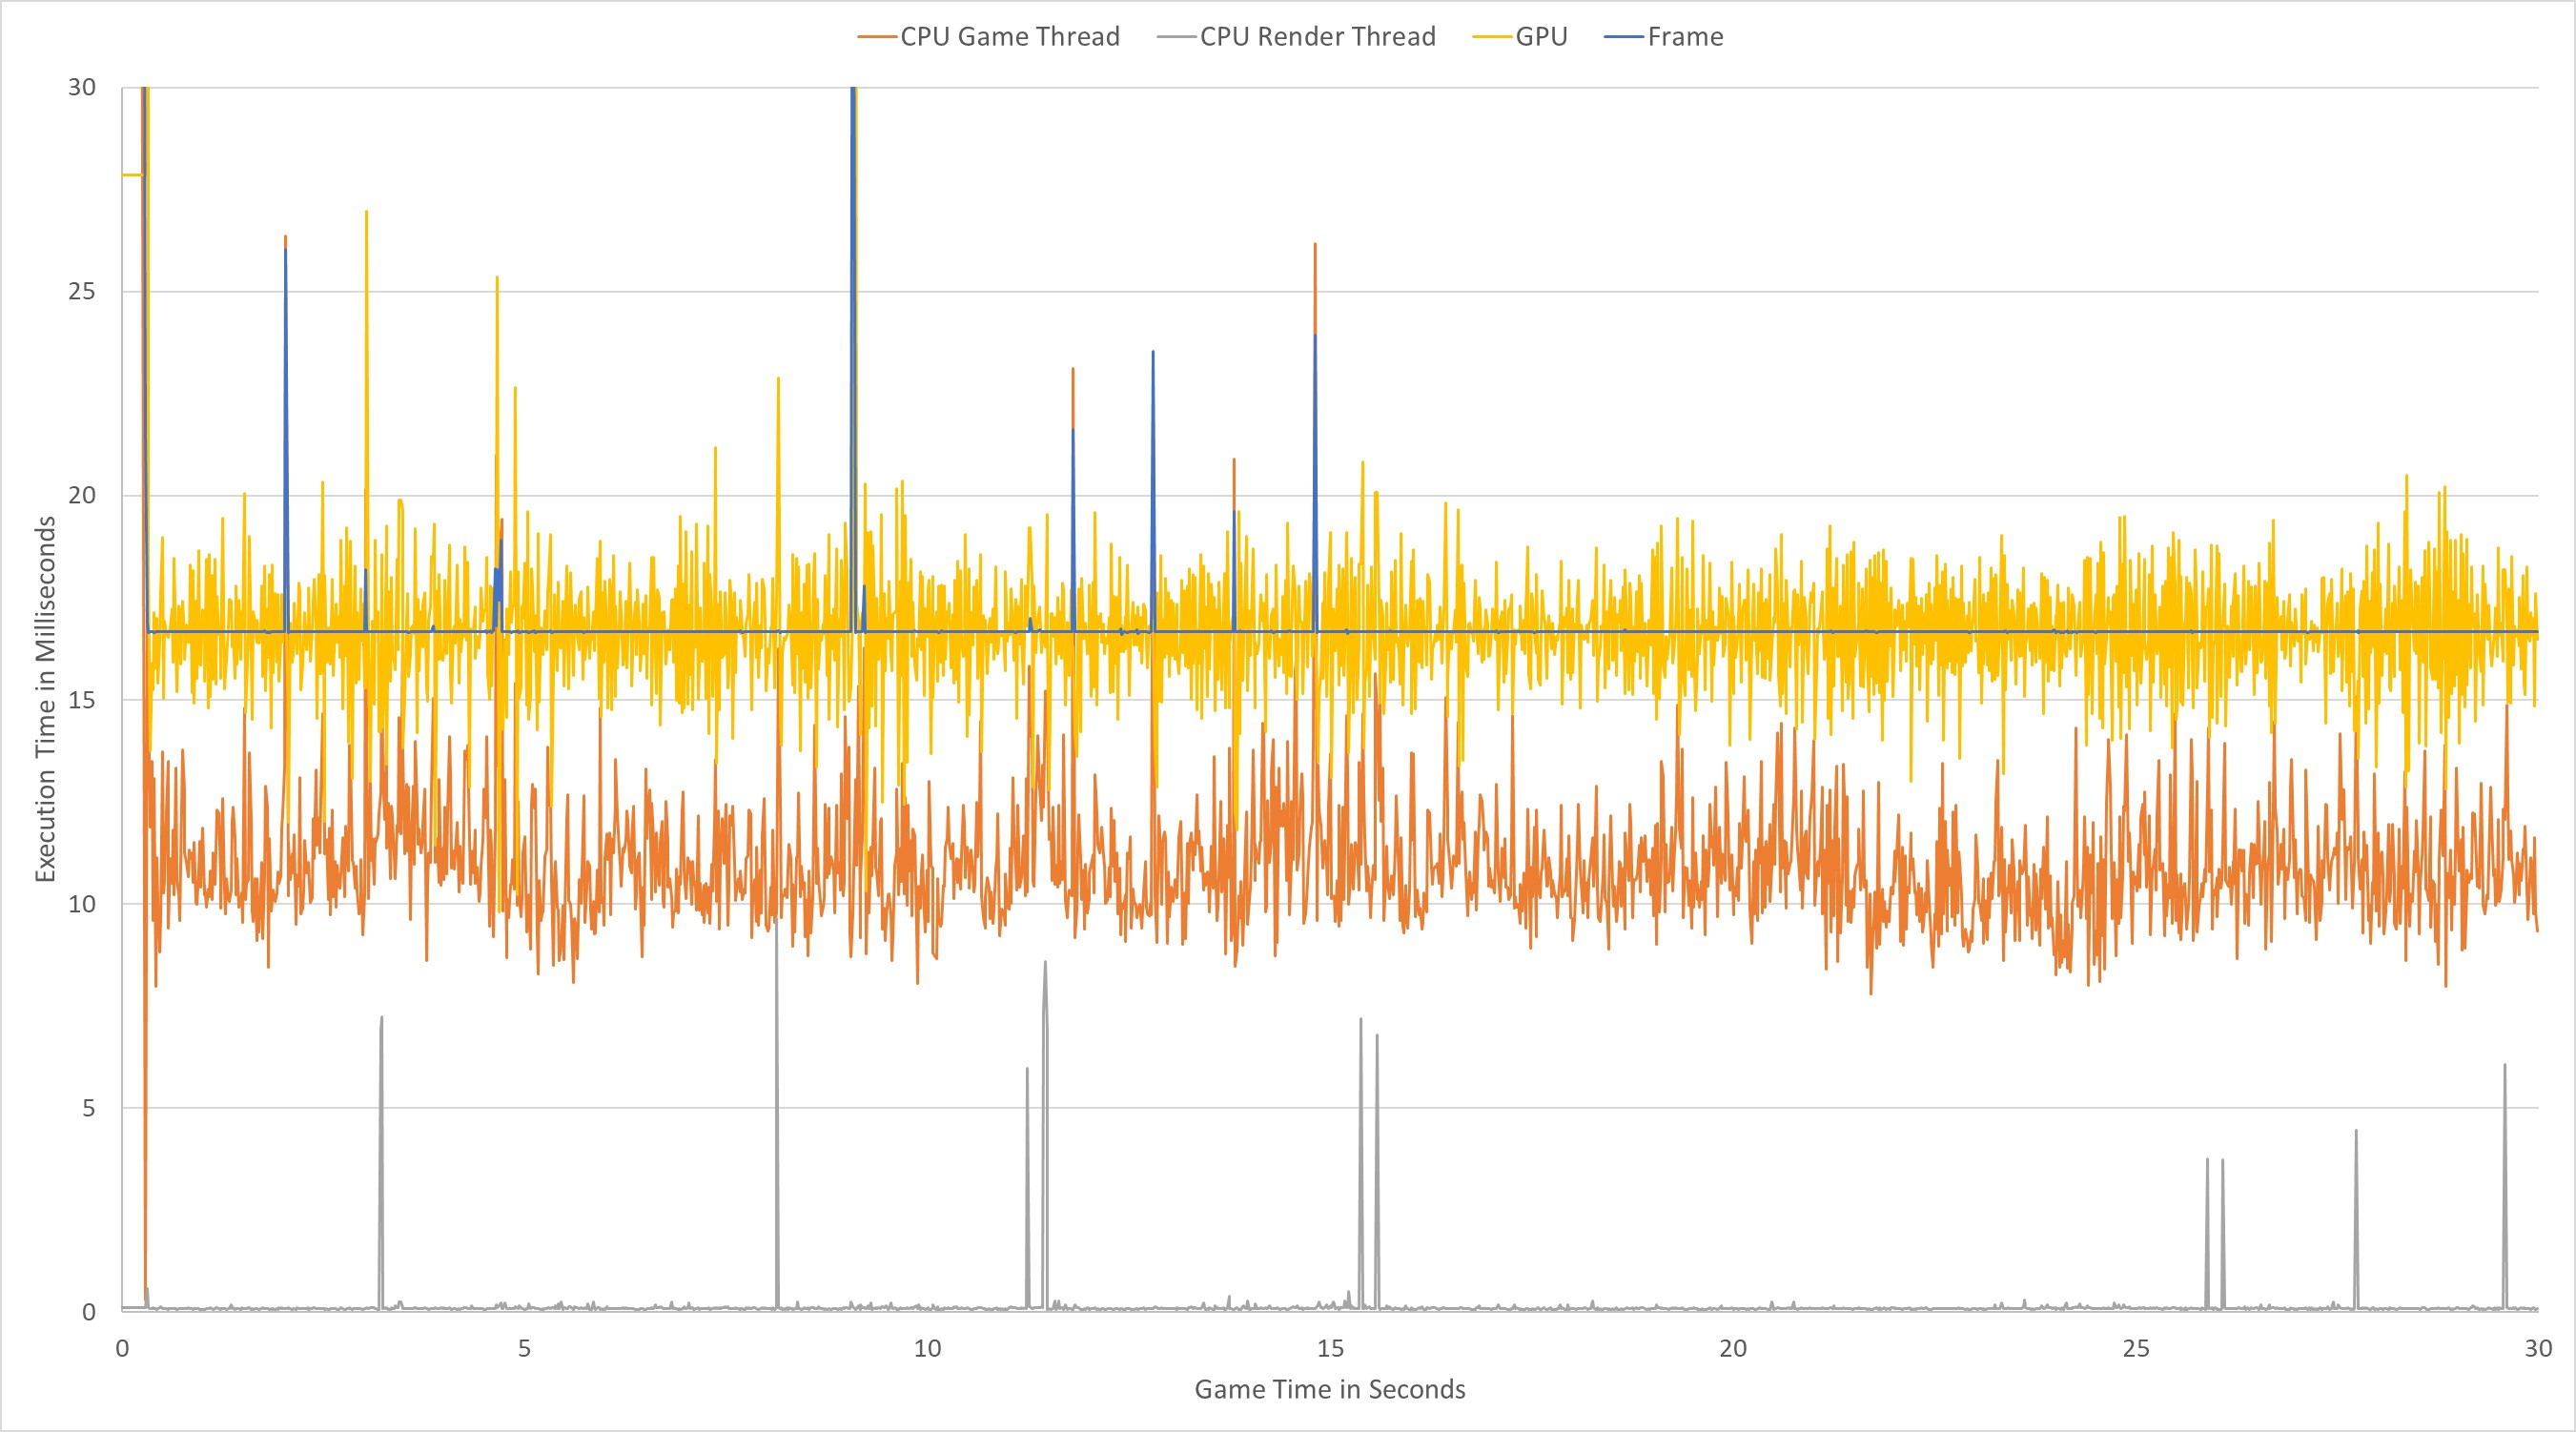
\includegraphics[width=1.0\linewidth]{PICs/Profiling/activated_plugin_no_tf_used}
	\caption{Profiling chart with the activated but not actively used TensorFlow Plugin for CPU.} \label{scenario::profiling_TF}
\end{figure}

Figure \ref{scenario::profiling_CPU} shows a profiling plot with an actively used \ac{TF} plugin and weapon generator in the game. The \ac{TF} plugin in this scenario was using the \ac{CPU} for computation. 
\begin{figure}[!ht]
	\centering
	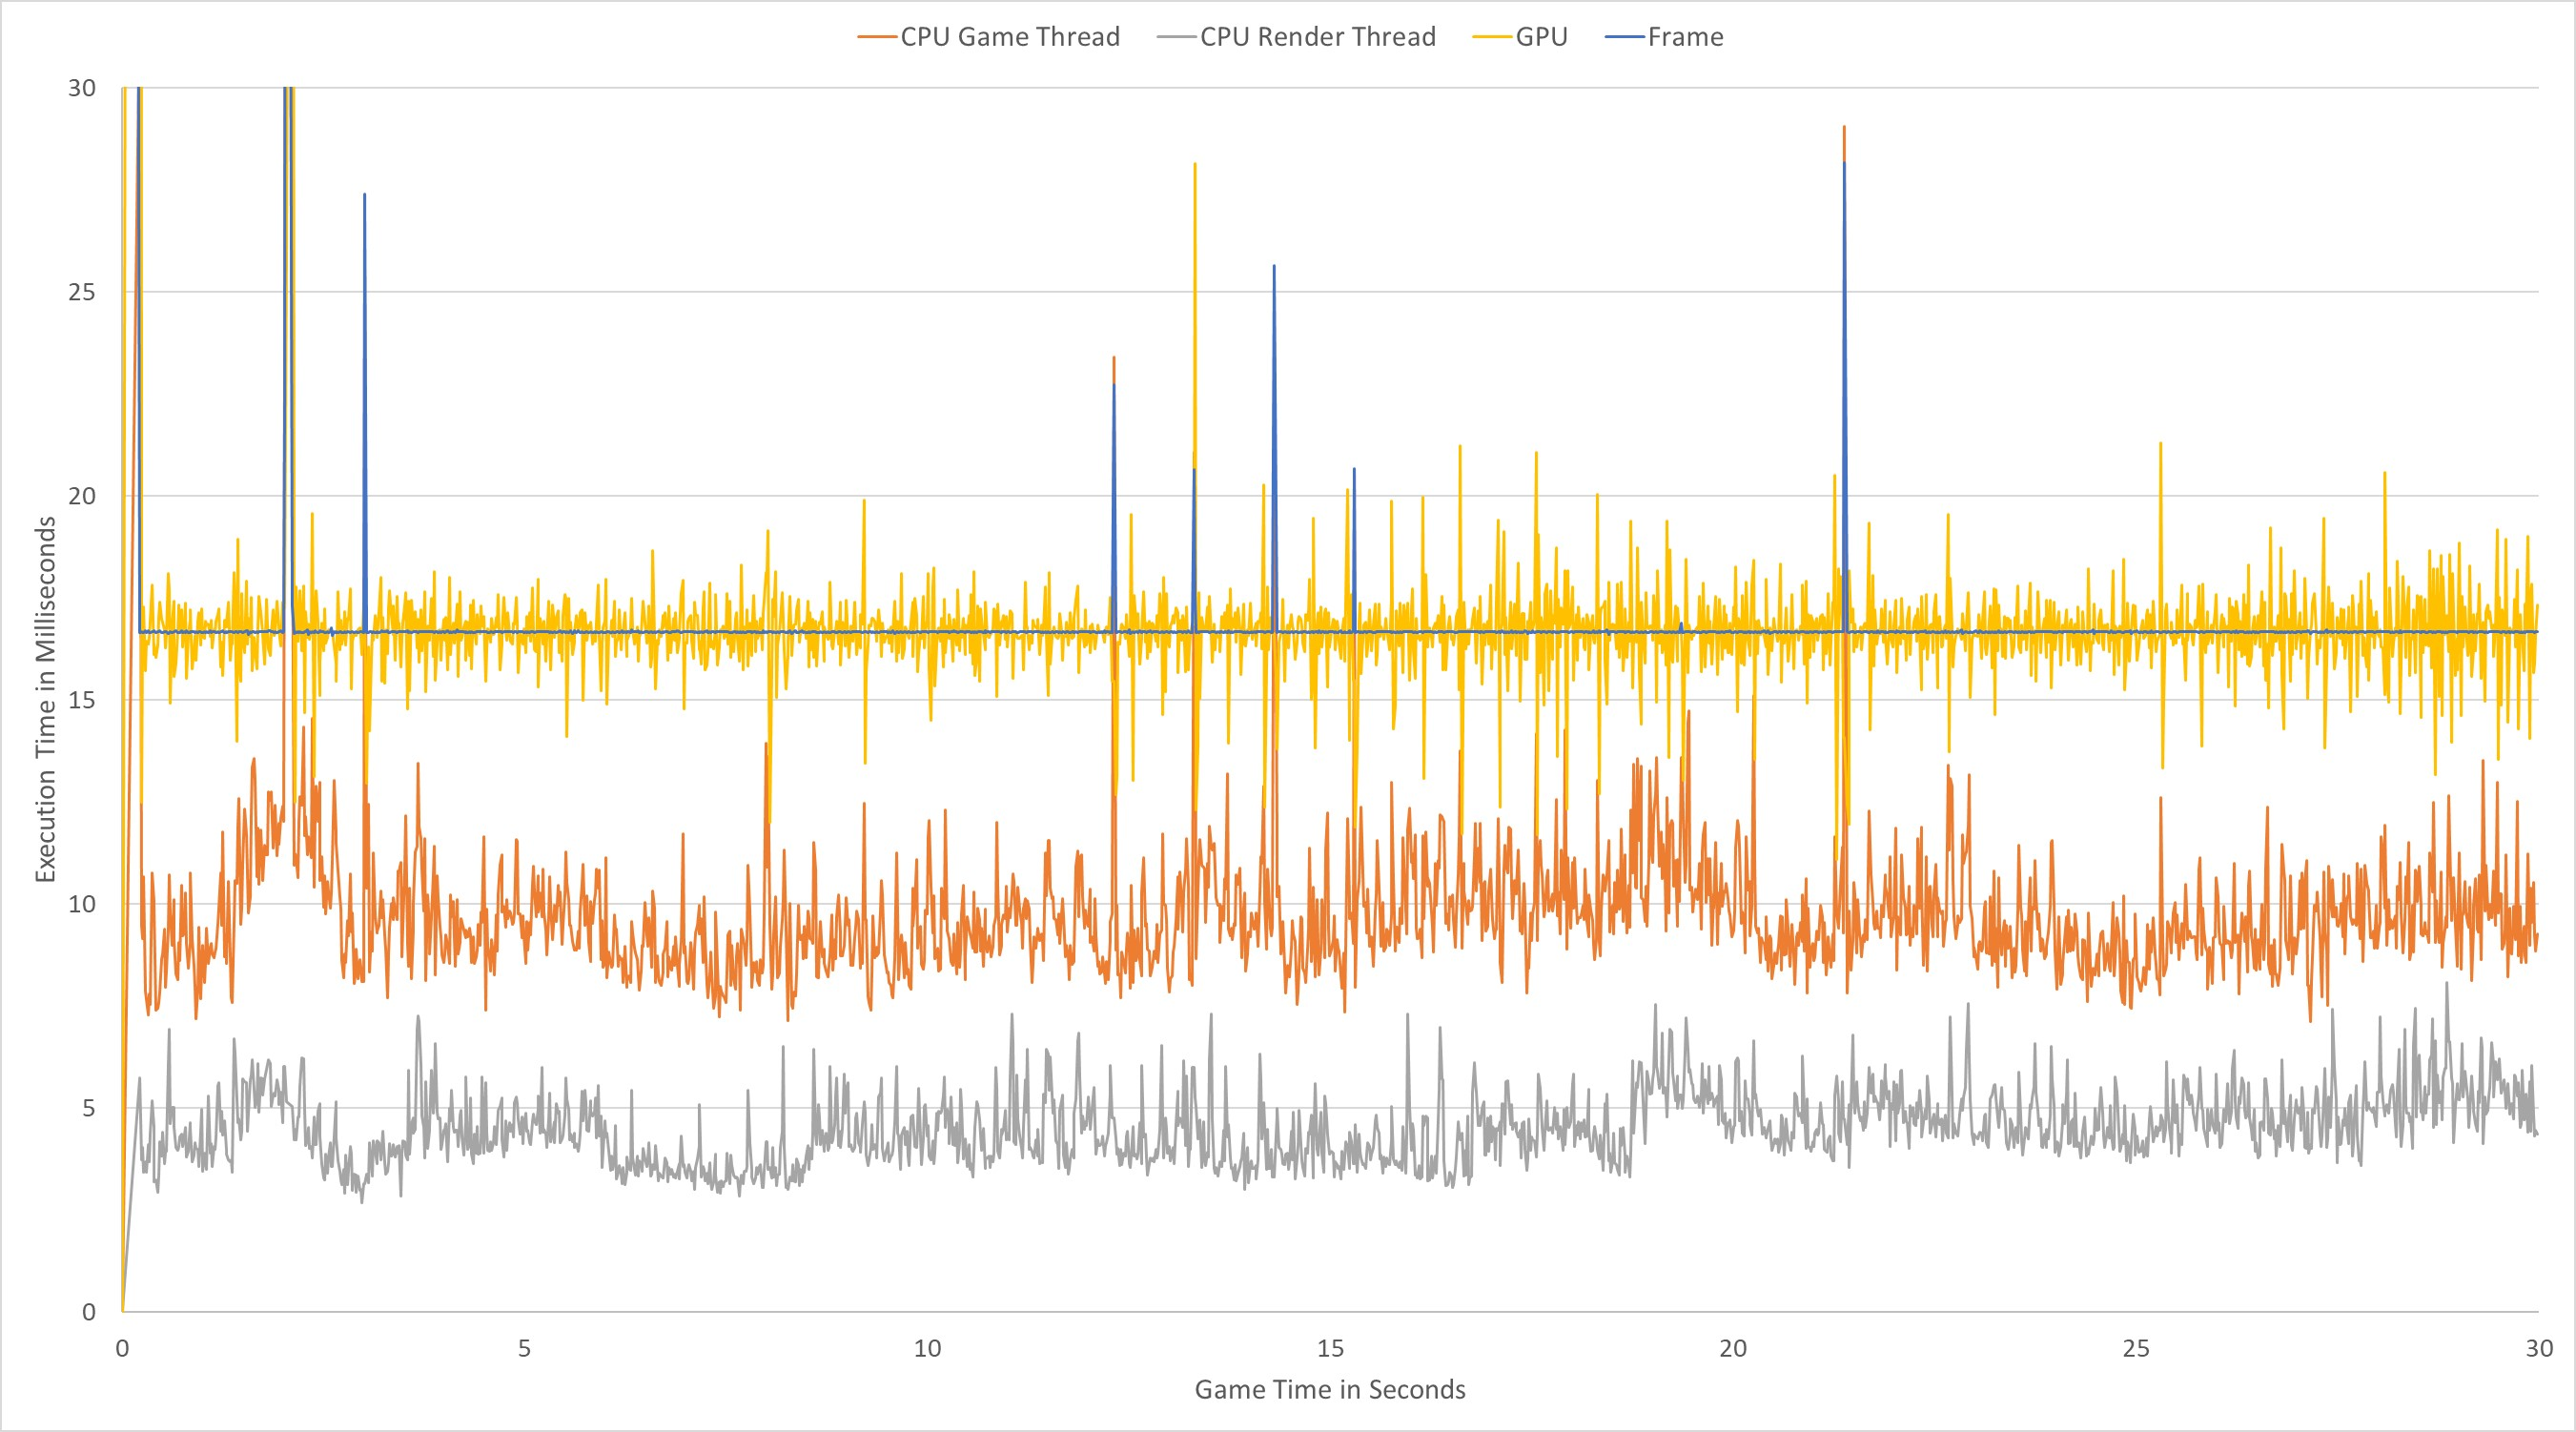
\includegraphics[width=1.0\linewidth]{PICs/Profiling/tf_cpu}
	\caption{Profiling chart with the actively used TensorFlow Plugin for CPU.} \label{scenario::profiling_CPU}
\end{figure}

Figure \ref{scenario::profiling_GPU} shows a profiling plot with an actively used \ac{TF} plugin and weapon generator in the game. The \ac{TF} plugin in this scenario was using the \ac{GPU} for computation.
\begin{figure}[!ht]
	\centering
	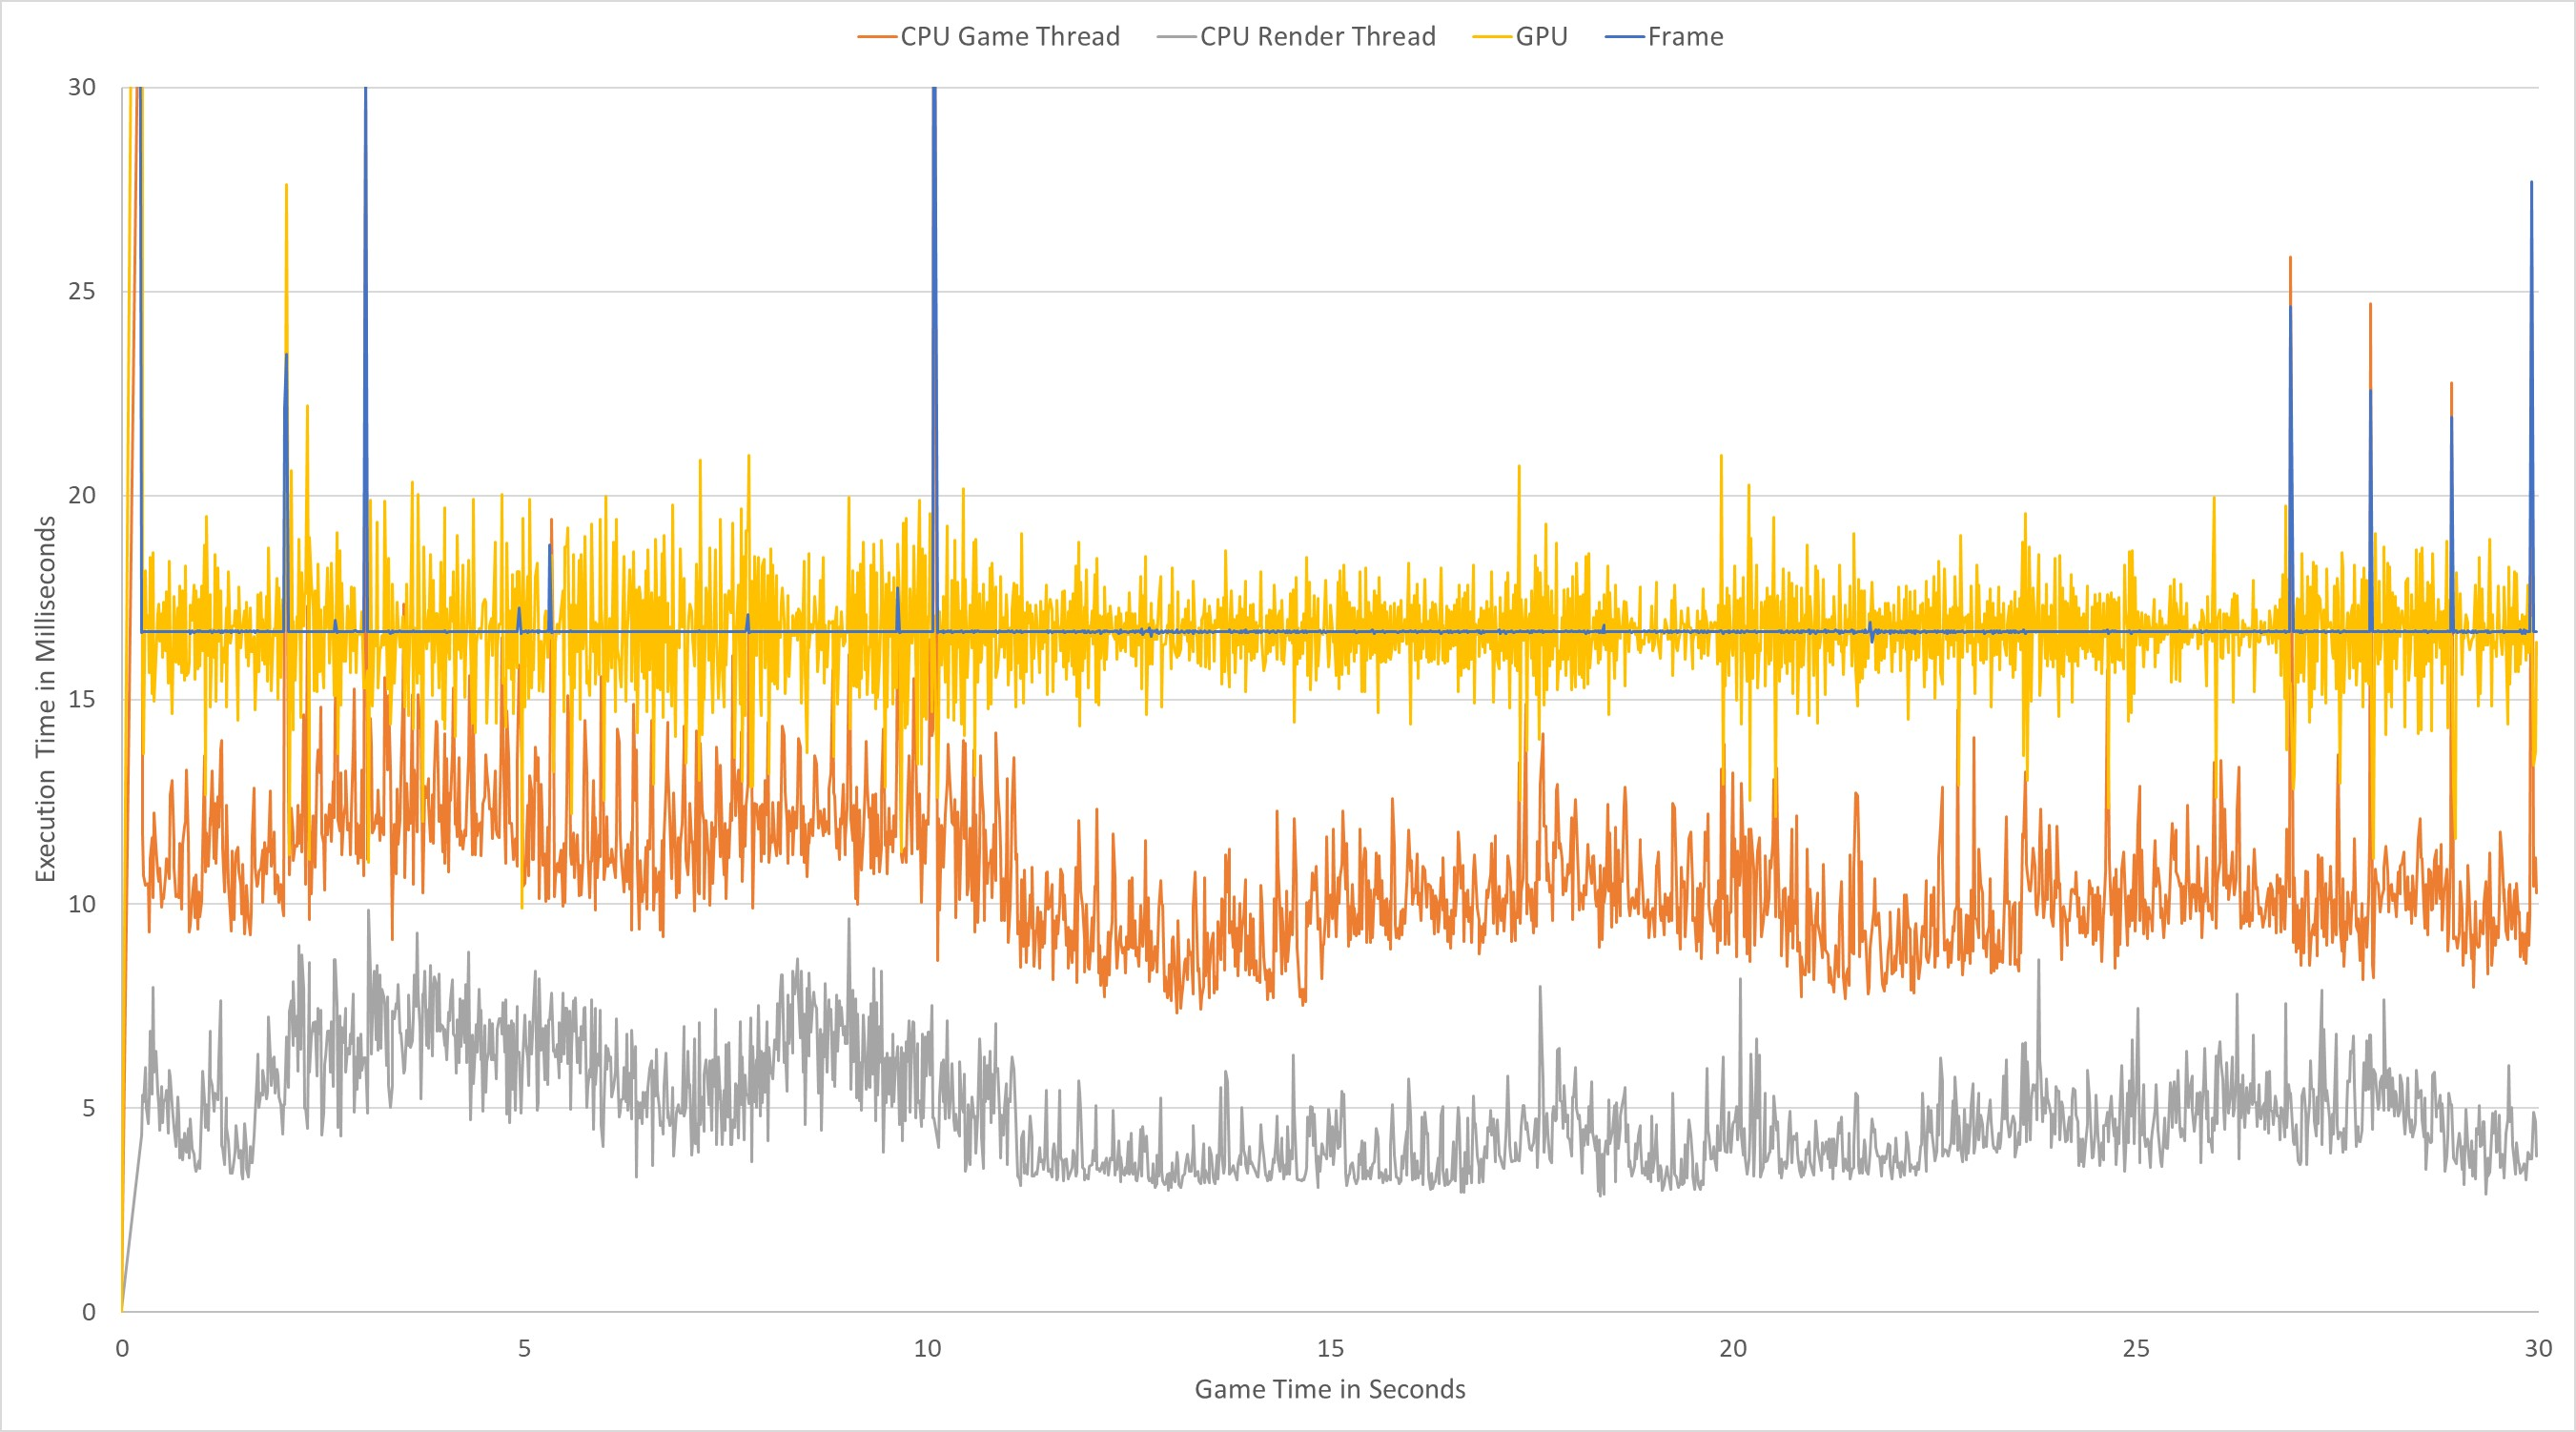
\includegraphics[width=1.0\linewidth]{PICs/Profiling/tf_gpu}
	\caption{Profiling chart with the actively used TensorFlow Plugin for GPU.} \label{scenario::profiling_GPU}
\end{figure}

\subsection{Conclusion}
The profiling charts show that there is a performance loss of about four milliseconds in the \ac{CPU} render thread when using the \ac{TF} plugin actively in the game. Moreover, it seems that the \ac{CPU} variant of the plugin works better than the \ac{GPU} variant in this case. This advantage might be because the \ac{TF} plugin uses \ac{CPU} multi-threading for the setup, training, and input processing tasks whereas the \ac{GPU} variant interrupts the \ac{GPU} from time to time because it needs to obtain the calculated tensors from \ac{TF} - but that is just an assumption and cannot be evidenced by facts. Nevertheless, it should be noted that this profiling charts reflect only this specific use case and could have other performances with other use cases. 

However, this shows that it is not necessary that someone trains the model in advance and loads a trained model on the first start. This procedure would only be necessary if the training would include a high number of training epochs and would prevent the player from using the mechanic. But this is not the case for this mechanic and therefore is not necessary.

%
% ------------------------------- NEW CHAPTER ------------------------------- %
%
\clearpage
\chapter{Conclusion}
The idea of this master thesis was to explore the possibilities of \ac{PCGML} as a game mechanic with focus on their applications in video games. Its primary goal was to provide a demonstration of the possibilities as well as to address every aspect of developing a \ac{PCGML} game mechanic in standard used free-to-use game engines. Overall, it shall serve as a concise overview and primer for developing \ac{PCGML} game mechanics with a prototype development example workflow.

In particular, the thesis fulfills all of the demanded requirements from the listing of unique game mechanic ideas for \ac{PCGML} up to an in-depth development of a prototype in a game engine. The development of "\nameref{idea::changingWeapons}" approach shows the potential for \ac{PCGML} as a game mechanic in future work and helps curious developers to quickly dive into every knowledge necessary to start developing new games with \ac{PCGML} game mechanics. It shows the room for improvement and lists essential development considerations for implementing a \ac{PCGML} game mechanic, so that there are no unexpected mistakes. In summary, this thesis established and reflects an introduction and overall guideline for bringing \ac{PCGML} game mechanics into a game.

\section{Research Result}
The focus of this thesis was to provide theoretical possibilities for \ac{PCGML} game mechanics, a practical development example, a showcase that \ac{PCGML} game mechanics are suitable for a broad range of games and are not limited to particular genres. Chapter \ref{chapter::possibleGameMechanics} provides these possibilities and furthermore shows some pros and cons of a theoretical development. The game mechanic "\nameref{idea::changingWeapons}" was then implemented and introduced the development workflow of a \ac{PCGML} game mechanic. Overall, the thesis fulfilled all expectations of using \ac{PCGML} as a game mechanic and shows valuable research results.

\subsection{Theoretical Part}
The primary focus of the "\nameref{idea::changingWeapons}" game mechanic is a weapon generator which helps the player to obtain its objective of defeating the end boss AI of a game. Hence, the development of this generator shows developers necessary preparations such as the decision between possible game engines, the examination of hardware and software requirements, ML data acquisition, data preprocessing knowledge, and at last, addresses the specific learning problem which needs to be tackled by the \ac{ML} model. Moreover, it introduces some suitable models which could be used for the generator model and focuses on the most promising model.

\subsection{Practical Part}
The practical part of the development showed the necessary steps for data preprocessing, an  overview of a weapon data convenience class, the actual ML model implementation and some empirical observations of the working model used in the game, as well as the generator API and the weapon generator in the game itself.

The prototype showed that the intention of emerging the model in a specific direction works but is as not fixed as expected because of how the network initialization works. Therefore, weapons during the game emerge in different directions for every new game due to the initialization of the weights and biases which means the model always trains in another way. The solution to that problem would be the pretraining and loading of the model at the beginning of the game. Also, the weapons in the training dataset bias the model in a specific direction, for example, shotguns are limited in the dataset and therefore are not often generated. Appendix \ref{bf1::data::distributionCharts} shows the distribution of the weapons which is the reason for higher generation numbers for specific weapons. 

Research showed that there are dozens of possible network configurations for the ML model which means that it has still room for possible improvements. Nevertheless, the developed ML model works as intended and outputs the desired data. However, the model sometimes produces unusable data during the generation process which was avoidable with omitting the faulty data. Hence, this does not break the actual game since the generator API does not propagate the faulty data into the game. This problem is due to the small training dataset and is solvable with more data to train. Another open problem is that the model cannot always reproduce and predict categorical features very well for which a workaround was introduced by using the category with the highest value.

Last but not least, the profiling of the game shows that the used development configuration does not affect performance too much. That means that it is possible to develop much more detailed and sophisticated game mechanics with PCGML without significant performance losses. Nevertheless, the next chapter proposes a possible minimization of the performance loss.

\section{Future Work}
Now, there is plenty of room for improvement and future work when implementing PCGML game mechanics. If speaking of this particular use case of implementing a weapon generator then there are following improvements possible:
\begin{itemize}
	\item First of all, it would be possible to get rid of the TF plugin in UE4 with a full C++ UE4 ML plugin. This C++ plugin would probably save much performance because it would not rely on a Python plugin, the SocketIO plugin or TF itself. Of course, this would work even better with an engine integration of ML. Therefore, the only possible engine with that advantage could be Unity with their current ML plugin development since UE4 does not seem to show interest in an ML integration. 
	\item Another improvement of the game mechanic would be an increase or replacement of the weapons in the training dataset to refine the trained model. More weapons enable training of the model with much more training features, and therefore it can learn the underlying structure even better. \\
	Nevertheless, this would currently cause a necessary refactoring of all the code to integrate the new features.
	\item It would be a valuable improvement if the current classes would be extended to work as generic types of classes and ML models for more use cases than the prototype game. This generic implementation would enable designers to change features of a traditional FPS game weapon with, e.g., RPG like features of causing fire damage and burning on the hit enemy.
	\item The generation of different and new ammo types would also be a possible improvement since the current prototype only uses ray-tracing weapons instead of projectile weapons. This additional generation would enable a much more diverse game mechanic and experiences for the player. For example, the new ammo types could follow a specific movement pattern as used for the weapons in the game "Galactic Arms Race," described in Chapter \ref{pcgMechanicGames}.
	\item The weapon generator itself offers even more improvement. Currently, the generator does not limit any values which means that because of the retraining functionality of the model, the weapon can get extraordinary high damage and other values. These high values are still okay if its intended but most likely they should be trimmed before sending to the generator API or creating the new weapons for the player.
	\item The gameplay concept for using the weapon generator also offers space for improvement. In particular, it is so see how the weapon generator can be integrated into the gameplay in a more natural way than pressing a button and get a new weapon. For example, a possible concept would be for the player to call for reinforcements, and they will send you new random weapons. In this scenario, the player would need to hold on to his current weapon until the reinforcement has landed.
\end{itemize}
As someone can see, there are many possibilities with PCGML game mechanics. This thesis only shows an example game mechanic which was rather easy to implement but offers much more sophisticated game mechanics which enable improved player experience. It is now a further research question to find out whether the designs of the in Chapter \ref{chapter::possibleGameMechanics} introduced game mechanics will work out as intended or not.

%
% Hier beginnen die Verzeichnisse.
%
\clearpage
\ifthenelse{\equal{\FHTWCitationType}{HARVARD}}{}{\bibliographystyle{gerabbrv}}
\bibliography{Literatur}
\clearpage

% Das Abbildungsverzeichnis
\listoffigures
\clearpage

% Das Tabellenverzeichnis
\listoftables
\clearpage

% Das Quellcodeverzeichnis
\listofcode
\clearpage

\phantomsection
\addcontentsline{toc}{chapter}{\listacroname}
\chapter*{\listacroname}
\begin{acronym}[XXXXX]
	\acro{2D}{2-Dimensional}
	\acro{3D}{3-Dimensional}
	\acro{AE}{Autoencoder}
	\acro{AI}{Artificial Intelligence}
	\acro{ANN}{Artificial Neural Network}
	\acro{API}{Application Programming Interface}
	\acro{BF1}{Battlefield 1}
	\acro{CNN}{Convolutional Neural Network}
	\acro{CPU}{Central Processing Unit}
	\acro{CS:GO}{Counter-Strike: Global Offensive}
	\acro{FPS}{First Person Shooter}
	\acro{GAN}{Generative Adversarial Network}
	\acro{GB}{Gigabyte}
	\acro{GPU}{Graphics Processing Unit}
	\acro{HMM}{Hidden Markov Model}
	\acro{HUD}{Head-up Display}
	\acro{JSON}{JavaScript Object Notation}
	\acro{KNN}{K-Nearest Neighbor}
	\acro{LSTM}{Long Short-Term Memory Network}
	\acro{MDA}{Mechanics-Dynamics-Aesthetics}
	\acro{ML}{Machine Learning}
	\acro{MMORPG}{Massively Multiplayer Online Roleplay Game}
	\acro{NLP}{Natural Language Processing}
	\acro{NN}{Neural Network}
	\acro{NPC}{Non-playable Character}
	\acro{OS}{Operating System}
	\acro{PC}{Personal Computer}
    \acro{PCG}{Procedural Content Generation}
    \acro{PCGML}{Procedural Content Generation via Machine Learning}
    \acro{PvE}{Player versus Environment}
    \acro{RAM}{Random Access Memory}
    \acro{RPG}{Roleplay Game}
    \acro{RL}{Reinforcement Learning}
    \acro{RNG}{Random Number Generator}
    \acro{RNN}{Recurrent Neural Network}
    \acro{SVM}{Support Vector Machine}
    \acro{TF}{TensorFlow}
    \acro{UE4}{Unreal Engine 4}
    \acro{VAE}{Variational Autoencoder}
    \acro{VR}{Virtual Reality}
    \acro{WW1}{World War One}
    \acro{WWW}{World Wide Web}
\end{acronym}

%
% Hier beginnt der Anhang.
%
\clearpage
\appendix
\chapter{PCGML Game Mechanics Summary} \label{gameMechanicIdeaSummary}
\begin{longtable}[c]{p{4cm}|p{5.5cm}|p{5.5cm}|}
	\cline{2-3}
	                               & \textbf{Output}                                               & \textbf{Training}                                                                              \\ \hline

	%
	\endhead
		\multicolumn{1}{|p{4cm}|}{\textbf{\nameref{idea::rulesAndBehavior}}}       & Configuration of a game with all its game elements.  & Working configuration of a game.                                                      \\ \hline
		\multicolumn{1}{|p{4cm}|}{\textbf{\nameref{idea::changingWeapons}}}        & New and novel weapons.                               & Existing balanced and unbalanced weapons.                                             \\ \hline
		\multicolumn{1}{|p{4cm}|}{\textbf{\nameref{idea::changingPowers}} }        & New and novel powers.                                & Existing useful powers like magic spells.                                             \\ \hline
		\multicolumn{1}{|p{4cm}|}{\textbf{\nameref{idea::novelCars}}     }         & New and novel vehicles.                              & Existing balanced and useful vehicles for a specific environment.                     \\ \hline
		\multicolumn{1}{|p{4cm}|}{\textbf{\nameref{idea::solverWeapon}}}           & E.g., elements of a puzzle.                          & Object detection and example drawings.                                                \\ \hline
		\multicolumn{1}{|p{4cm}|}{\textbf{\nameref{idea::defeatTheEnemy}} }        & New and successful attack patterns.                  & Possible AI behavior such as attacks or movement for a specific environment.          \\ \hline
		\multicolumn{1}{|p{4cm}|}{\textbf{\nameref{idea::caughtInAThunderstorm}}}  & Lightning diffusion pattern.                         & Example diffusion pattern based on real weather data.                                 \\ \hline
		\multicolumn{1}{|p{4cm}|}{\textbf{\nameref{idea::trainToProgress}} }       & E.g., elements of a puzzle such as a key for a lock. & No need for training due to training with player.                                     \\ \hline
		\multicolumn{1}{|p{4cm}|}{\textbf{\nameref{idea::buildingWithAssistance}}} & Incomplete elements which allow modification.        & Samples of incomplete elements for the game.                                          \\ \hline
		\multicolumn{1}{|p{4cm}|}{\textbf{\nameref{idea::exploringCoWorker}}}      & Terrain generation or manipulation.                  & Example terrains based on player progress.                                            \\ \hline
		\multicolumn{1}{|p{4cm}|}{\textbf{\nameref{idea::observeAndLearn}}}        & Terrain generation or manipulation.                  & Example terrains.                                                                     \\ \hline
		\multicolumn{1}{|p{4cm}|}{\textbf{\nameref{idea::expressYourself}} }       & Storyline with events and choices connected to it.   & Configuration and story for possible games.                                           \\ \hline
		\multicolumn{1}{|p{4cm}|}{\textbf{\nameref{idea::bigBossHelper}} }         & Terrain generation and modification.                 & Example terrains with obstacles based on a player behavior in a specific environment. \\ \hline
		\multicolumn{1}{|p{4cm}|}{\textbf{\nameref{idea::figureItOut}} }           & E.g., elements of a puzzle.                          & Example puzzle elements to progress in a game.                                        \\ \hline

	\caption{PCGML game mechanic training and output summary.}
\end{longtable}

\chapter{Battlefield 1 Community Weapon Analytic Dump Parameters} \label{bf1::dumpParams}
\begin{longtable}[c]{|l|p{10.5cm}|}
	\hline
	\textbf{Parameter}     & \textbf{Explanation}                                                                                                           \\ \hline
	\endhead
	%
	ADSCrouchBaseMax       & Maximum shot spread if the character is crouching, not moving, and aiming down sight.                                          \\ \hline
	ADSCrouchBaseMin       & Minimum shot spread if the character is crouching, not moving, and aiming down sight.                                          \\ \hline
	ADSCrouchBaseSpreadDec & The decrease of shot spread if the character is crouching, not moving, and aiming down sight.                                  \\ \hline
	ADSCrouchBaseSpreadInc & The increase of shot spread if the character is crouching, not moving, and aiming down sight.                                  \\ \hline
	ADSCrouchMoveMax       & Maximum shot spread if the character is crouching, moving, and aiming down sight.                                              \\ \hline
	ADSCrouchMoveMin       & Minimum shot spread if the character is crouching, moving, and aiming down sight.                                              \\ \hline
	ADSCrouchMoveSpreadDec & The decrease of shot spread if the character is crouching, moving, and aiming down sight.                                      \\ \hline
	ADSCrouchMoveSpreadInc & The increase of shot spread if the character is crouching, moving, and aiming down sight.                                      \\ \hline
	ADSProneBaseMax        & Maximum shot spread if the character is lying, not moving, and aiming down sight.                                              \\ \hline
	ADSProneBaseMin        & Minimum shot spread if the character is lying, not moving, and aiming down sight.                                              \\ \hline
	ADSProneBaseSpreadDec  & The decrease of shot spread if the character is lying, not moving, and aiming down sight.                                      \\ \hline
	ADSProneBaseSpreadInc  & The increase of shot spread if the character is lying, not moving, and aiming down sight.                                      \\ \hline
	ADSProneMoveMax        & Maximum shot spread if the character is lying, moving, and aiming down sight.                                                  \\ \hline
	ADSProneMoveMin        & Minimum shot spread if the character is lying, moving, and aiming down sight.                                                  \\ \hline
	ADSProneMoveSpreadDec  & The decrease of shot spread if the character is lying, moving, and aiming down sight.                                          \\ \hline
	ADSProneMoveSpreadInc  & The increase of shot spread if the character is lying, moving, and aiming down sight.                                          \\ \hline
	ADSRecoilDec           & Weapon recoil decrease if the character is aiming down sight.                                                                  \\ \hline
	ADSRecoilLeft          & Weapon recoil to the left if the character is aiming down sight.                                                               \\ \hline
	ADSRecoilRight         & Weapon recoil to the right if the character is aiming down sight.                                                              \\ \hline
	ADSRecoilUp            & Weapon recoil upwards if the character is aiming down sight.                                                                   \\ \hline
	ADSStandBaseMax        & Maximum shot spread if the character is standing, not moving, and aiming down sight.                                           \\ \hline
	ADSStandBaseMin        & Minimum shot spread if the character is standing, not moving, and aiming down sight.                                           \\ \hline
	ADSStandBaseSpreadDec  & The decrease of shot spread if the character is standing, not moving, and aiming down sight.                                   \\ \hline
	ADSStandBaseSpreadInc  & The increase of shot spread if the character is standing, not moving, and aiming down sight.                                   \\ \hline
	ADSStandMoveMax        & Maximum shot spread if the character is standing, moving, and aiming down sight.                                               \\ \hline
	ADSStandMoveMin        & Minimum shot spread if the character is standing, moving, and aiming down sight.                                               \\ \hline
	ADSStandMoveSpreadDec  & The decrease of shot spread if the character is standing, moving, and aiming down sight.                                       \\ \hline
	ADSStandMoveSpreadInc  & The increase of shot spread if the character is standing, moving, and aiming down sight.                                       \\ \hline
	AltDeployTime          & Remnant parameter gathered by the script.                                                                                      \\ \hline
	Ammo                   & Type of ammunition used in the weapon.                                                                                         \\ \hline
	Bdrop                  & A bullet's drop due to gravity.                                                                                                \\ \hline
	BRoF                   & The rate of fire in burst mode.                                                                                                \\ \hline
	BridgeDelay            & Delay added to the first reloaded single bullet.                                                                               \\ \hline
	Class                  & Defines which character class in Battlefield 1 uses this weapon.                                                               \\ \hline
	Damages                & Damage points applied, listed based on distance.                                                                               \\ \hline
	DeployTime             & Is the time it takes to weapon be able to fire after switching to said weapon.                                                 \\ \hline
	Dmg\_distances         & The distances in correlation to each damage entry in the "Damages" parameter.                                                  \\ \hline
	Drag                   & A bullet's drag.                                                                                                               \\ \hline
	Edmg                   & Least applied damage points.                                                                                                   \\ \hline
	FirstShotADSSpreadMul  & Spread multiplier applied on the first shot or the final shot in burst mode if the character is aiming down sight.             \\ \hline
	FirstShotHIPSpreadMul  & Spread multiplier applied on the first shot or the final shot in burst mode if the character is not aiming down sight.         \\ \hline
	FirstShotRecoilMul     & Recoil multiplier applied on the first shot or the final shot in burst mode.                                                   \\ \hline
	FirstSingleBulletTime  & The time it takes to reload the first bullet if single bullet reloading is available.                                          \\ \hline
	HIPCrouchBaseMax       & Maximum shot spread if the character is crouching, not moving, and not aiming down sight.                                      \\ \hline
	HIPCrouchBaseMin       & Minimum shot spread if the character is crouching, not moving, and not aiming down sight.                                      \\ \hline
	HIPCrouchBaseSpreadDec & The decrease of shot spread if the character is crouching, not moving, and not aiming down sight.                              \\ \hline
	HIPCrouchBaseSpreadInc & The increase of shot spread if the character is crouching, not moving, and not aiming down sight.                              \\ \hline
	HIPCrouchMoveMax       & Maximum shot spread if the character is crouching, moving, and not aiming down sight.                                          \\ \hline
	HIPCrouchMoveMin       & Minimum shot spread if the character is crouching, moving, and not aiming down sight.                                          \\ \hline
	HIPCrouchMoveSpreadDec & The decrease of shot spread if the character is crouching, moving, and not aiming down sight.                                  \\ \hline
	HIPCrouchMoveSpreadInc & The increase of shot spread if the character is crouching, moving, and not aiming down sight.                                  \\ \hline
	HIPProneBaseMax        & Maximum shot spread if the character is lying, not moving, and not aiming down sight.                                          \\ \hline
	HIPProneBaseMin        & Minimum shot spread if the character is lying, not moving, and not aiming down sight.                                          \\ \hline
	HIPProneBaseSpreadDec  & The decrease of shot spread if the character is lying, not moving, and not aiming down sight.                                  \\ \hline
	HIPProneBaseSpreadInc  & The increase of shot spread if the character is lying, not moving, and not aiming down sight.                                  \\ \hline
	HIPProneMoveMax        & Maximum shot spread if the character is lying, moving, and not aiming down sight.                                              \\ \hline
	HIPProneMoveMin        & Minimum shot spread if the character is lying, moving, and not aiming down sight.                                              \\ \hline
	HIPProneMoveSpreadDec  & The decrease of shot spread if the character is lying, moving, and not aiming down sight.                                      \\ \hline
	HIPProneMoveSpreadInc  & The increase of shot spread if the character is lying, moving, and not aiming down sight.                                      \\ \hline
	HIPRecoilDec           & Weapon recoil decrease if the character is not aiming down sight.                                                              \\ \hline
	HIPRecoilLeft          & Weapon recoil lower bound of random recoil if the character is not aiming down sight.                                          \\ \hline
	HIPRecoilRight         & Weapon recoil upper bound of random recoil if the character is not aiming down sight.                                          \\ \hline
	HIPRecoilUp            & Weapon recoil upwards if the character is not aiming down sight.                                                               \\ \hline
	HIPStandBaseMax        & Maximum shot spread if the character is standing, not moving, and not aiming down sight.                                       \\ \hline
	HIPStandBaseMin        & Minimum shot spread if the character is standing, not moving, and not aiming down sight.                                       \\ \hline
	HIPStandBaseSpreadDec  & The decrease of shot spread if the character is standing, not moving, and not aiming down sight.                               \\ \hline
	HIPStandBaseSpreadInc  & The increase of shot spread if the character is standing, not moving, and not aiming down sight.                               \\ \hline
	HIPStandMoveMax        & Maximum shot spread if the character is standing, moving, and not aiming down sight.                                           \\ \hline
	HIPStandMoveMin        & Minimum shot spread if the character is standing, moving, and not aiming down sight.                                           \\ \hline
	HIPStandMoveSpreadDec  & The decrease of shot spread if the character is standing, moving, and not aiming down sight.                                   \\ \hline
	HIPStandMoveSpreadInc  & The increase of shot spread if the character is standing, moving, and not aiming down sight.                                   \\ \hline
	HorDispersion          & Horizontal pellet dispersion (for shotguns).                                                                                   \\ \hline
	InitialSpeed           & Muzzle velocity.                                                                                                               \\ \hline
	MagSize                & Size of one magazine.                                                                                                          \\ \hline
	NumBulletsReloaded     & The Number of bullets reloaded when using magazines or strip clips.                                                            \\ \hline
	PostReloadDelay        & Post-reload delay after reloading mechanic ends.                                                                               \\ \hline
	ReloadDelay            & Pre-reload delay before actual reloading mechanic begins. (Not strip clip reload or single bullet reload)                      \\ \hline
	ReloadEmpty            & The time it takes if the magazine is empty.                                                                                    \\ \hline
	ReloadLeft             & The time it takes if the magazine there is still some ammo left.                                                               \\ \hline
	ReloadThrs             & The fraction of the reload time before someone can swap weapons and still receives fully reloaded ammo.                        \\ \hline
	RoF                    & The rate of fire.                                                                                                              \\ \hline
	SDmg                   & Maximum damage points without taking distance into account.                                                                    \\ \hline
	ShotsPerBurst          & The number of pellets of one shot in burst mode.                                                                               \\ \hline
	ShotsPerShell          & The number of pellets of one shot.                                                                                             \\ \hline
	SingleBulletReloadTime & The time it takes to reload single bullets after "FirstSingleBulletTime" was applied. (Semi-automatic and bolt-action weapons) \\ \hline
	StripClipSize          & The number of bullets reloaded by "strip" clips.                                                                               \\ \hline
	StripReloadTime        & The time it takes to reload the stripper clip.                                                                                 \\ \hline
	TimeToLive             & Seconds how long the bullet lives before despawning.                                                                           \\ \hline
	VerDispersion          & Vertical pellet dispersion (for shotguns).                                                                                     \\ \hline
	\_\_CustomReload\_\_   & This parameter only applies in super individual cases.                                                                         \\ \hline
	\caption{Battlefield 1 community weapon analytic dump data parameter.}
\end{longtable}

\chapter{Battlefield 1 Weapon Distribution Charts} \label{bf1::data::distributionCharts}
\begin{figure}[!ht]
	\centering
	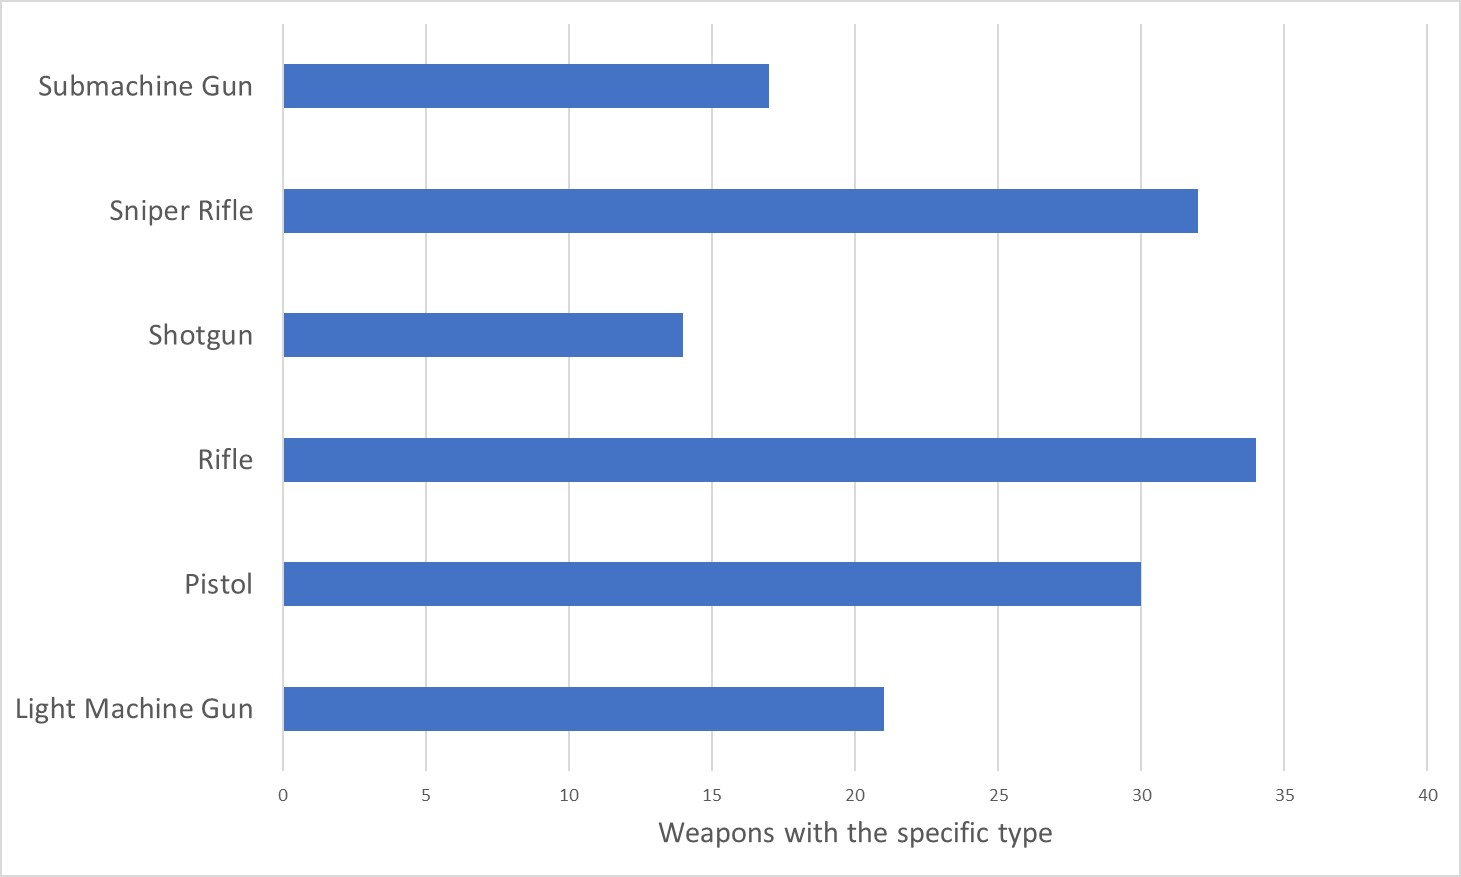
\includegraphics[width=0.8\linewidth]{PICs/weapon_type_distribution_chart}
	\caption{Distribution of weapon types in the Battlefield 1 weapon dataset.}
\end{figure}
\begin{figure}[!ht]
	\centering
	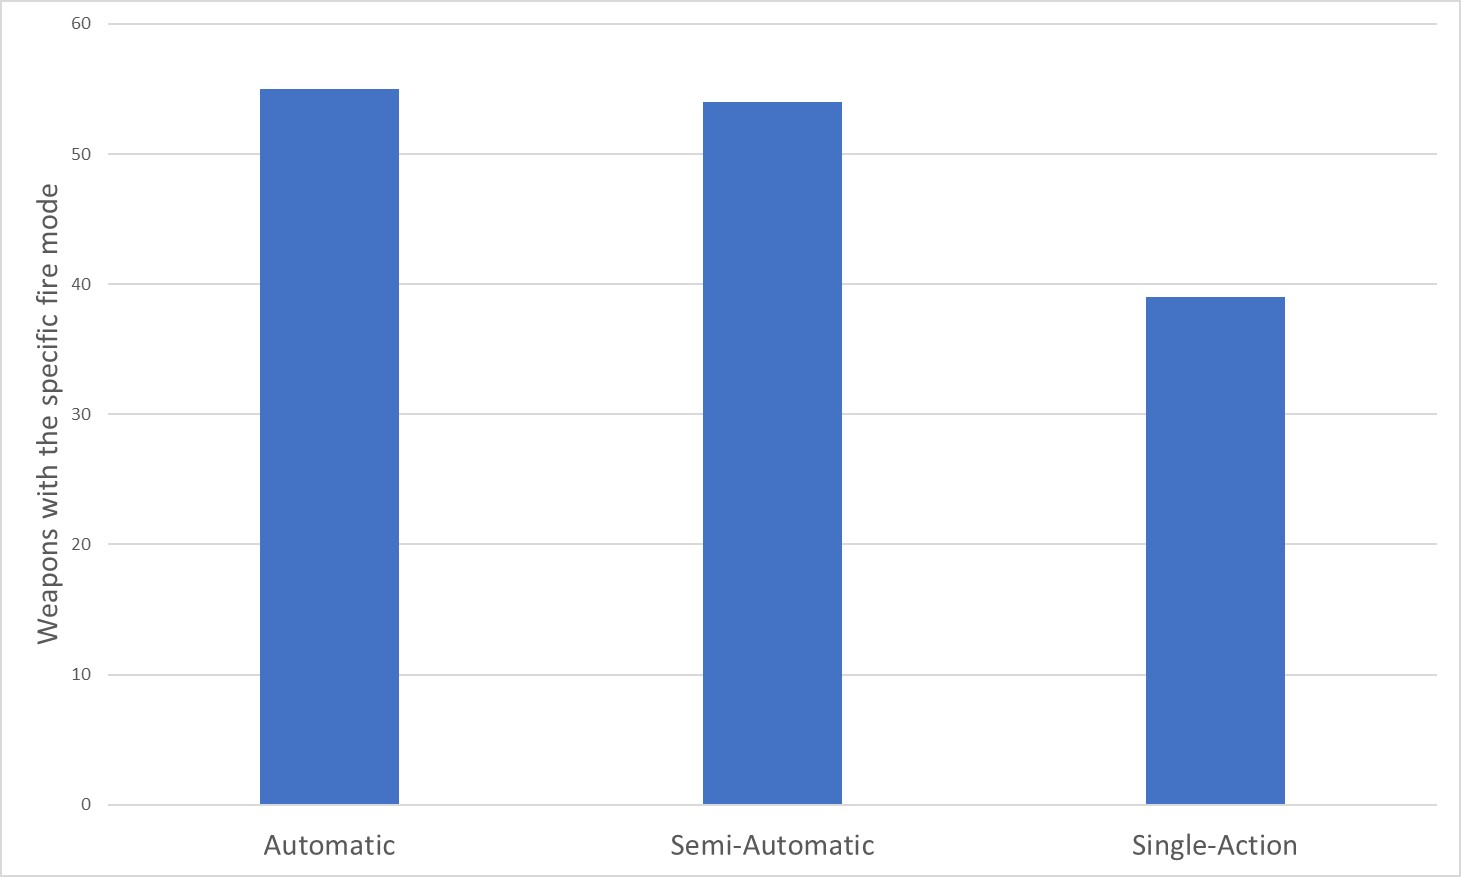
\includegraphics[width=0.8\linewidth]{PICs/weapon_fire_mode_distribution_chart}
	\caption{Distribution of weapon fire modes in the Battlefield 1 weapon dataset.}
\end{figure}
\end{document}